\documentclass[12pt]{report}
\usepackage[utf8x]{inputenc}
\usepackage[greek,english]{babel}
\usepackage[margin=1in]{geometry}
\usepackage{amsfonts, amsmath, amssymb}
\usepackage{amsmath,amsfonts,amssymb,amsthm,epsfig,epstopdf,titling,url,array}
\usepackage{mathtools}
\usepackage[none]{hyphenat}
\usepackage{fancyhdr}
\usepackage{times}
\usepackage{enumitem}
\usepackage{verbatim}
\usepackage{setspace}


\renewcommand{\baselinestretch}{1.5} 

\usepackage{subcaption}
\usepackage{tikz}
\usetikzlibrary{shapes,backgrounds,shapes,positioning,petri,topaths}
\usetikzlibrary{automata,positioning}

%\usepackage{pstricks}
%\usepackage{pst-all}

\usepackage{color}
\usepackage{listings} 
\usepackage{xspace}  % to allow for text macros that don't eat space 



\lstdefinelanguage{Sage}[]{Python}
{morekeywords={True,False,sage,singular},
sensitive=true}
\lstset{frame=none,
          showtabs=False,
          showspaces=False,
          showstringspaces=False,
          commentstyle={\ttfamily\color{dredcolor}},
          keywordstyle={\ttfamily\color{dbluecolor}\bfseries},
          stringstyle ={\ttfamily\color{dgraycolor}\bfseries},
          language = Sage,
	  basicstyle={\small \ttfamily},
	  aboveskip=.3em,
	  belowskip=.1em
          }
\definecolor{dblackcolor}{rgb}{0.0,0.0,0.0}
\definecolor{dbluecolor}{rgb}{.01,.02,0.7}
\definecolor{dredcolor}{rgb}{0.8,0,0}
\definecolor{dgraycolor}{rgb}{0.30,0.3,0.30}
\newcommand{\dblue}{\color{dbluecolor}\bf}
\newcommand{\dred}{\color{dredcolor}\bf}
\newcommand{\dblack}{\color{dblackcolor}\bf}

\renewcommand{\emph}[1]{{\dblack{#1}}}

\newcommand{\Sage}{{\color{dbluecolor}\sf Sage}\xspace}

\pagestyle{fancy}
%\fancyhead{}
%\fancyfoot{}
%\newcommand\tab[1][1cm]{\hspace*{#1}}
\DeclarePairedDelimiter\ceil{\lceil}{\rceil}

\newtheorem{prop}{Proposition}
\newtheorem{lemma}{Lemma}
\newtheorem*{remark}{Remark}
\newtheorem{cor}{Corollary}

\newtheorem{mythm}{Theorem}[section]
%\theoremstyle{definition}
\newtheorem{defn}[mythm]{Definition}
\newtheorem{exa}[mythm]{Example}

%\fancyfoot[C]{\thepage}
%\theoremstyle{definition}
%\newtheorem{defn}[thm]{Definition}



\newenvironment{dedication}
  {%\clearpage           % we want a new page          %% I commented this
   \thispagestyle{empty}% no header and footer
   \vspace*{\stretch{1}}% some space at the top
   \itshape             % the text is in italics
   \raggedleft          % flush to the right margin
  }
  {\par % end the paragraph
   \vspace{\stretch{3}} % space at bottom is three times that at the top
   \clearpage           % finish off the page
  }


\begin{document}

\title{The Goulden-Jackson cluster method}

\author{Dimitrios Noulas}

\maketitle

\begin{dedication}
    
    \par   %% or a blank line


    \vspace{\baselineskip}
    \textgreek{Για τον αδερφό μου Θωμά και}\\
    \textgreek{την γιαγιά μου Αικατερίνη}
  \end{dedication}

\chapter*{Prologue}

The current dissertation was undertaken in order to fullfil the graduation requirements in the Department of Informatics at the University of Piraeus, as well as to expand my own mathematical knowledge. It's scope is to research about a known theorem in combinatorics, the ideas behind it and how it can be applied to solve different kinds of enumeration problems. This research is also complemented by python scripts at the last sections which help solve some of the problems with the use of this theorem.

At this point, I would like to thank my supervisor, Prof. Aristidis Sapounakis for giving me the opportunity to undertake this dissertation based on an interesting research question. I would also like to express my gratitude towards Prof. Ioannis Tasoulas for all of his help, the research material he provided me as well as his guidance and all the countless hours we spent cooperating or just discussing about mathematics.
%%%%%%%%%%%%%%%%%%%%%%%%%%%%%%%%%%%%%%%%%%%%%%%%%%%%%%%%%%%%%%%

\chapter*{Introduction}

The focus of this dissertation is the efficient enumeration of words with certain subwords based on the Goulden-Jackson cluster theorem.

In the first chapter, some preliminary notions are given from combinatorics and graph theory and different mathematical techniques are demonstrated on words.

The second chapter is split in two cases, the enumeration of a single pattern and the enumeration of multiple patterns simultaneously. For both cases, words as mathematical objects are extended to the notion of marked words from which a special case arises, the clusters. In more depth, it can be seen in both cases how the use of generating functions help achieve the intended enumeration, however, deriving a generating function for words is not always straightforward. This is where the necessary connections are made between the generating function of words and the generating function of marked words, thus demonstrating the inclusion-exclusion approach. Furthermore, the derivation of the second is proven to be dependent on the generating function of clusters, hence reducing the original problem to a straightforward one.

In the last chapter, different kinds of applications of the Goulden Jackson cluster method take place. The first kind is how problems of enumeration unrelated, at first, to words can be solved using this method. The second application is on self-avoiding walks which are related to physics. The method here is used to count a certain type of patterns which turn to overcount self-avoiding walks, thus creating an upper bound for a known constant. The final application is on biology, where the method is used to provide theoretical statistics for words such that biologists can compare them to the actual statistics on words from genomes.

Finally, Python and Sage scripts complement this dissertation, on which most of the applications in the 3rd chapter are based on.
%%%%%%%%%%%%%%%%%%%%%%%%%%%%%%%%%%%%%%%%%%%%%%%%%%%%%%%%%%%%%%%


\tableofcontents


\chapter{Preliminaries}
%\section{Goulden Jackson}

\begin{comment}
\section{Formal Power Series}
In this section we recall the basics regarding formal power series. We follow the text of Goulden and Jackson []


{\color{blue} Let $R=(R,+,*)$ be a ring with unity. The \textbf{characteristic} of $R$ is the smallest positive integer n such that: \[na=\underbrace{a+a+a+\cdots+a}_\text{\textit{n} times}=0 \quad  \textrm{ for all  } a \in \textrm{R}\]
We say that $R$ is of characteristic zero if and only if: \[na=0 \iff n=0 \quad \textrm{or} \quad a=0 \quad \textrm{where} \quad n \in \mathbb{Z} \quad \textrm{and} \quad a\in R \] 
}

{\color{red} Let $X=\{x_1,x_2,\ldots,x_r\}$ be a set of commutative \textit{indeterminates}.
Every expression of the form: 
\[ F(x)=c_0 x^0 + c_1 x^1 + \cdots +c_n x^n = \sum_{i=0}^{n}c_i x^i  \quad\textrm{where} \quad c_i \in R\textrm{,} \quad x \in\textit{X} \quad \textrm{and } x^i \textrm{ is a monomial.}\]
is called a {\textit{formal power series}} with respect to the indeterminate $x$.}

The set of all formal power series with respect to the indeterminate $x$ is denoted by $R[[x]]$ and $c_i$ is called the coefficient of $x^i$ denoted by $[x^i]F(x)$. 

Two formal power series $F(x),G(x)$ are equal if and only if \([x^n]F(x)=[x^n]G(x) \textrm{ for all } n \in \mathbb{N}\). 

A formal power series $F(x)$ is $0$ if and only if $[x^n]F(x)=0$ for all $n \in \mathbb{N}$.

Let $F(x),G(x)\in R[[x]]$. We define the (formal) sum of $F,G$ as shown: \[\big[x^n\big](F+G)(x)=\big[x^n\big]F(x)+\big[x^n\big]G(x) \quad \forall n\in \mathbb{N}\]
and their (formal) product as follows: \[ \big[x^n\big]F(x) * \big[x^n\big]G(x) = \big[x^n\big](FG)(x)=\sum_{i=0}^{n}\big[x^i\big]F(x)\big[x^{n-i}\big]G(x) \quad \forall n\in \mathbb{N}\]

\begin{prop}
Let $R$ be a ring with characteristic zero. The set $(R\big[\big[x\big]\big],+,*)$ is a commutative ring with unity $x^0$.
\end{prop}

\begin{proof} First, we need to prove that $(R\big[\big[x\big]\big],+)$ is an abelian group.

Let $F(x),G(x),H(x) \in R\big[\big[x\big]\big]$ such that $F(x)=\sum_{i=0}^{n}a_i x^i , G(x)=\sum_{i=0}^{n}b_i x^i$ and $ H(x)=\sum_{i=0}^{n}c_i x^i$ where $a_i,b_i,c_i \in R \quad \forall i \in \big[n\big]$.
\begin{align*}
\big[x^n\big]F(x)+\big[x^n\big]G(x)
& =\big[x^n\big](F+G)(x)=a_n + b_n = b_n + a_n 
 =\big[x^n\big]G(x)+\big[x^n\big]F(x) 
\end{align*} thus the $+$ operation is commutative. 
\begin{align*}
\Big(\big[x^n\big]F(x) + \big[x^n\big]G(x)\Big) + \big[x^n\big]H(x)
& =\big[x^n\big](F+G)(x)+\big[x^n\big]H(x) \\
& = (a_n + b_n) + c_n \\
& = a_n + b_n + c_n  \\
& = \big[x^n\big](F+G+H)(x)
\end{align*}

\begin{align*}
\big[x^n\big]F(x) + \Big(\big[x^n\big]G(x) + \big[x^n\big]H(x)\Big)
& =\big[x^n\big](F)(x)+\big[x^n\big](G+H)(x) \\
& = a_n + (b_n + c_n) \\
& = a_n + b_n + c_n \\
& = \big[x^n\big](F+G+H)(x)
\end{align*}
thus the $+$ operation is also associative.

The identity element of $(R\big[\big[x\big]\big],+)$ is $ E(x)=\sum_{i=0}^{n}e_i x^i$ where $E(x)\in R\big[\big[x\big]\big], e_i \in R, e_i=0$ for all $i\in [n]$. Indeed: \[\big[x^n\big]F(x) + \big[x^n\big]E(x)=  \big[x^n\big]E(x) + \big[x^n\big]F(x)  = 0 + a_n = a_n =  \big[x^n\big]F(x)\]

For all $F(x) \in R\big[\big[x\big]\big]$ there exists an inverse element $-F(x) \in R\big[\big[x\big]\big]$ regarding the $+$ operation, where $-F(x)=\sum_{i=0}^{n}a'_i x^i, \quad a'_i = -a_i \quad \forall i \in [n]$. Indeed:
\[ \big[x^n\big]F(x) + \big[x^n\big]\big(-F(x)\big) = \big[x^n\big]\big(-F(x)\big) + \big[x^n\big]F(x) = a'_n + a_n = (-a_n) + a_n = 0 = \big[x^n\big]E(x) \]
hence, we have proven that $(R\big[\big[x\big]\big],+)$ is an abelian group.\\
 
The $*$ operation is associative:\[ \big[x^n\big]F(x) * \Big(\big[x^n\big]G(x) * \big[x^n\big]H(x)\Big) = \sum_{i=0}^{n}\big[x^i\big]F(x)\big[x^{n-1}\big](GH)(x) =\] \[\sum_{i=0}^{n}\big[x^i\big]F(x)\sum_{k=0}^{n-i}\big[x^k\big]G(x)\big[x^{n-i-k}\big]H(x)= \sum_{i=0}^{n}\sum_{k=0}^{n-i}\big[x^i\big]F(x)\big[x^k\big]G(x)\big[x^{n-i-k}\big]H(x) \]\\
\[ \Big(\big[x^n\big]F(x) * \big[x^n\big]G(x)\Big) * \big[x^n\big]H(x) = \sum_{i=0}^{n}\big[x^i\big]F(x)\big[x^{n-1}\big](GH)(x) =\] \[\sum_{i=0}^{n}\big[x^i\big](FG)(x)\big[x^{n-i}\big]H(x)= \sum_{i=0}^{n}\sum_{k=0}^{i}\big[x^k\big]F(x)\big[x^{i-k}\big]G(x)\big[x^{n-i}\big]H(x)=\]
\[ \sum_{k=0}^{n}\sum_{i=k}^{n}\big[x^k\big]F(x)\big[x^{i-k}\big]G(x)\big[x^{n-i}\big]H(x)=\sum_{k=0}^{n}\sum_{m=0}^{n-k}\big[x^k\big]F(x)\big[x^m\big]G(x)\big[x^{n-m-k}\big]H(x)\] (if we let $m=i-k$)

Therefore: $\Big(\big[x^n\big]F(x) * \big[x^n\big]G(x)\Big) * \big[x^n\big]H(x)=\big[x^n\big]F(x) * \Big(\big[x^n\big]G(x) * \big[x^n\big]H(x)\Big)$\\

The $*$ operation is also commutative:
\[ \big[x^n\big]F(x)*\big[x^n\big]G(x)=\sum_{i=0}^{n}\big[x^i\big]F(x)\big[x^{n-i}\big]G(x)=\sum_{i=0}^{n}a_i b_{n-i} \]

\[\big[x^n\big]G(x)*\big[x^n\big]F(x)=\sum_{i=0}^{n}\big[x^i\big]G(x)\big[x^{n-i}\big]F(x)=\sum_{i=0}^{n}b_i a_{n-i}=\sum_{i=0}^{n}a_{n-i} b_{i}=\sum_{m=0}^{n}a_m b_{n-m}\] (if we let $m=n-i$)\\
Therefore: $\big[x^n\big]F(x)*\big[x^n\big]G(x)=\big[x^n\big]G(x)*\big[x^n\big]F(x)$\\

The $*$ operation is distributive over the $+$ operation: 
\[ \Big(\big[x^n\big]F(x) + \big[x^n\big]G(x)\Big) * \big[x^n\big]H(x)=\big[x^n\big](F+G)(x) * \big[x^n\big]H(x) = \sum_{i=0}^{n}\big[x^i\big](F+G)(x)\big[x^{n-i}\big]H(x) =\]
\[ \sum_{i=0}^{n}(a_i + b_i)c_{n-i}= \sum_{i=0}^{n}(a_i c_{n-i} + b_i c_{n-i}) = \sum_{i=0}^{n}a_i c_{n-i}+ \sum_{i=0}^{n}b_i c_{n-i} = \]
 \[ \sum_{i=0}^{n}\big[x^i\big]F(x)\big[x^{n-i}\big]H(x) + \sum_{i=0}^{n}\big[x^i\big]G(x)\big[x^{n-i}\big]H(x)=\]
\[\big[x^n\big]F(x) * \big[x^n\big]H(x) + \big[x^n\big]G(x) * \big[x^n\big]H(x)\]

Hence, we have proven that $(R\big[\big[x\big]\big],+,*)$ is a commutative ring.

\[ \big[x^n\big]F(x) * x^0 = \sum_{i=0}^{n}\big[x^i\big]F(x)\big[x^{n-i}\big]x^0 = \sum_{i=0}^{n}\big[x^n\big]F(x) \delta_{n,i} = \big[x^n\big]F(x) \delta_{n,n} = \big[x^n\big]F(x) \] thus, $x^0$ is the ring's unity.

\end{proof}

An $R$ ring is called an \textbf{integral domain} if and only if:
\[ ab = 0 \iff a = 0 \quad \textrm{or} \quad b=0, \quad a,b \in R\]

\begin{prop}
$R\big[\big[x\big]\big]$ is an integral domain if and only if $R$ is an integral domain.
\end{prop}

\begin{proof}


Let $F(x),G(x) \in R\big[\big[x\big]\big], \quad F(x)=\sum_{i=0}^{n}a_i , \quad G(x)=\sum_{i=0}^{n}b_i$ and $(FG)(x) = 0$
\[(FG)(x) = 0 \iff \big[x^n\big](FG)(x) = 0 \quad \forall n \in \mathbb{N}\]
\[\iff \sum_{i=0}^{n}\big[x^i\big]F(x)\big[x^{n-i}\big]G(x) = 0 \quad \forall n \in \mathbb{N}\]
\[\iff \sum_{i=0}^{n}a_i b_{n-i} = 0 \quad \forall n \in \mathbb{N} \]

For $n=0$: \[a_0 b_0 = 0\]
\[\iff a_0=0 \quad \textrm{or} \quad b_0 =0\](Should $R$ be an integral domain.)
Without loss of generality let $a_0=0$. We distinguish the two following cases:
either $b_0 \neq 0$ or $b_0=0$.\\
Regarding the first case, we can prove that $a_n=0$ by induction for all $n \in \mathbb{N}$:

Base case: If $n=0$ then $a_0=0$.

Inductive hypothesis: Suppose that $a_n=0$ holds for all values of $n$ up to some $k, k \geq 0$.

Inductive step: Let $n=k+1$ then:
\[a_0 b_{k+1} + a_1 b_{k} + ... + a_k b_1 + a_{k+1} b_0 = 0\]
\[\Rightarrow a_{k+1} b_0 = 0\]
\[\Rightarrow a_{k+1} = 0, \quad \textrm{since} \quad b \neq 0\]
Thus, $F(x) = 0$. We have proved in this case that $R\big[\big[x\big]\big]$ is an integral domain, since $ (FG)(x)=0 \iff F(x) = 0$ (or $G(x) = 0$, should we choose $b_0$ instead of $a_0$ to be zero).\\
Regarding the second case where both $a_0,b_0=0$, we will prove by induction that if $a_i,b_i=0 \quad$ for all $ i \in [n]$ then $a_{m+1} b_{m+1}=0$ for all $m \in \mathbb{N}$ where $m = \ceil{\frac{n}{2}}$ and $n$ is an even number. We need $n$ to be even in order for $a_m b_m$ to appear in the sum.

Base case: If $n=0$ we have $m=0, a_0 b_0=0$ which is true.

Inductive hypothesis: Suppose that the above proposition holds for all values of $n$ up to some even $k+2, k \geq 0$.

Inductive step: Let $n=k+4$ then :
\[a_0 b_{k+4} + a_1 b_{k+3} + ...+ a_{m+1} b_{m+3} + a_{m+2}b_{m+2} +a_{m+3} b_{m+1}+... + a_{k+3} b_1 + a_{k+4} b_0 = 0\]
\[\Rightarrow a_{m+2}b_{m+2} = 0\]

From the above, we have proven that $a_{m+1}b_{m+1}$ will always be equal to zero if all previous $a_i,b_i$ are equal to zero for all $i \in [n]$. From there, we will have to treat $a_{m+1}b_{m+1}$ as we did with $a_0 b_0$ in the first case. As a result, we will either prove that one of the formal power series equals to zero or both $a_{m+1}$ and $b_{m+1}$ are equal to zero. Hence, we will meet our requirements for $a_{m+1}b_{m+1}$ to be equal to zero and in an inductive way we will always meet our requirements for $a_{\ceil{\frac{n}{2}}}b_{\ceil{\frac{n}{2}}}$ to be equal to zero for all $n \in \mathbb{N}$, since also our base case holds as: $a_0=b_0=a_1 b_1 = 0$, in order to make a recursion to the first case.
%\tab
\end{proof}


\begin{prop} Let $M$ be the set of all $m \times m$ matrices with elements in a ring $R$ with unity. Then, $(M,+,\cdot)$ is a ring with unity.
\end{prop}

\begin{proof}
?? well known?? %well known? ιδιοτητες δακτυλιου
\end{proof}

\begin{prop} $det(I-xA)$ is invertible for every $A \in M$ such that $det(I-xA) \in R[[x]]$.
\end{prop}

\begin{proof}
It is well known that a formal series is invertible if and only if it has a nonzero constant term. Therefore:
\begin{align*}
det(I-xA) &= det(I-\frac{1}{z} A)  \\
&= det(\frac{1}{z}(zI-A))  \\
&= (\frac{1}{z})^n det(zI-A) \\
&= \frac{(-1)^n}{z^n} det(A-zI) \\
&= \frac{(-1)^n}{z^n} ((-1)^n z^n + b_{n-1} z^{n-1} + \ldots + b_1 z + b_0 ) \\
&= 1 + (-1)^n (b_{n-1} z^{-1} + \ldots + b_1 z^{-(n-1)} + b_0 z^{-n} ) \\
&= 1 + (-1)^n (b_{n-1} x + \ldots + b_1 x^{n-1} + b_0 x^n )
\end{align*}
where $b_0,b_1,\ldots,b_n \in R$.
\end{proof}

\begin{prop}
$\sum\limits_{n=0} A^n x^n = (I-xA)^{-1}$ where $I-xA, \sum\limits_{n=0} A^n x^n \in M[[x]]$.
\end{prop}

\begin{proof}
\begin{align*}
[x^n](I-xA) \sum\limits_{j=0} A^j x^j &= \sum\limits_{k=0}^n [x^k] (I-xA) [x^{n-k}] \sum\limits_{j=0} A^j x^j \\
&= \begin{cases} I A^0, & n=0 \\
I A^n + (-A) A^{n-1}, & n\geq 1 \end{cases} \\
&= \begin{cases} I, & n=0 \\
0, & n\geq 1 \end{cases}
\end{align*}
\end{proof}

\begin{cor}
It follows from the previous proposition that if $(A)_{ij}$ is the $i,j$-th element of a matrix $A \in M$ then $(\sum\limits_{n=0} A^n x^n)_{ij}=((I-xA)^{-1})_{ij}$.
\end{cor}



\section{Words and formal series}

Let $L$ be a finite alphabet and $L^*$ be the set all words using letters from the alphabet $L$ (including the {\em empty word}, i.e., the word having no letters, denoted by $\varepsilon$).

The set $L^*$ together with the {\em concatenation} or {\em product} operation $*$ of words is a {\em monoid}, where the empty word $\varepsilon$ acts as the identity element.

The binary operation of concatenation $*$ can be extended to subsets of $L^*$ by defining for $X, Y \subseteq L^*$ that
\[ X Y = \{ xy | x \in X, y \in Y \}.  \]

Let $K$ be a ring with unity. A formal series $f$ with coefficients in $K$ and variables in $L$ is a mapping $f: L^* \to K$. The set of all these series is denoted by $K[[L]]$. The value of $f$ on the word $w \in L^*$, i.e. $f(w)$, is denoted by $[w] f$ and is called the coefficient of $w$ in $f$.

The operations of sum and product of two formal series $f, g \in K[[L]]$ are defined as follows:
\[ [w] (f + g) = [w] f + [w] g \]
\[ [w] f g = \sum\limits_{w = u v} [u] f [v] g \]
for any $w \in L^*$.

The set $K[[L]]$ equipped with the above two operations is a ring. This ring has a unity that is the series ${\bf 1}$, where $[w] {\bf 1} = \begin{cases} 1, & \textrm{ if } w = \epsilon, \\ 0, & \textrm{ if } w \ne \epsilon \end{cases}$, where $1$ is the unity of $K$.


Let $u, v, w$ be some words in $L^*$. We can define the formal sum of $u, v$ 
\[ u + v \]
where the sum is associative and commutative, so that
\[ u + v = v + u \]
\[ (u + v) + w = u + (v + w).\]

We can also define the product of two formal sums of words by requiring that the distributive law also holds for words:
\[ u (v + w) = u v + u w. \]

\end{comment}



\section{Patterns in words}


Let $L$ be a finite alphabet and let $L^*$ be the set of all words using letters from the alphabet $L$ (including the {\em empty word, i.e. the word having no letters, denoted by $\varepsilon$). Now,  let $w, \tau$ be some words in $L^*$.

\begin{defn}[Occurrences of patterns]
We say that the word $\tau$, called in this context {\em pattern} or {\em string}, {\em occurs} in $w$ iff there exist $v, u \in L^*$, such that 
\[ w = v \tau u,\] 
equivalently if $w = w_1 w_2 \cdots w_n$ and $\tau = \tau_1 \tau_2 \cdots \tau_k$ then there exists $j \in [n-k]$ such that
\[ w_{j - 1 + i} = \tau_i \textrm{ for all } i \in [k], \]
in this case we say that there is an {\em occurrence of $\tau$}, or {\em $\tau$ occurs at position $j$ in $w$}.
The number of occurrences of the pattern $\tau$ in $w$, is denoted $|w|_\tau$. If $w$ has no occurrences of $\tau$, then we say that $w$ {\em avoids} the pattern $\tau$. Two occurences of a pattern $\tau$ at positions $j_1$, $j_2$ in $w$ {\em overlap} iff $|j_1 - j_2| < |\tau|$. Similarly, two occurences of two patterns $\tau_1$, $\tau_2$ at positions $j_1$, $j_2$ in $w$ with $j_1 < j_2$ {\em overlap} iff $|j_1 - j_2| < |\tau_1|$.
\end{defn}

\begin{exa}
The word $w = a b b a b b a b b a a a b b$ has two occurrences of the pattern $\tau_1 = b a b b$ at positions $3$ and $6$, i.e. $|w|_\tau = 2$; these two occurrences overlap in $w$ since $|3 - 6| < |\tau_1| = 4$, while $w$ avoids the pattern $\tau_2 = b b b$.
\end{exa}

\begin{defn}[Periodic words]
A word $w = w_1 w_2 \cdots w_n$, $n \ge 1$, is called {\em periodic} iff there exists a positive integer $p \in [n-1]$ such that $w_{p+i} = w_{i}$ for all $i \in [n-p]$.
The number $p$ is called the {\em period} of $w$. 
\end{defn}

\begin{exa} The word $w = a b b a b b a b b a a a b b$ is periodic since for $p = 11$ we have that $w_{11 + i} = w_i$ for all $i \in [14-11] = [3]$, so that $w$ has period $11$. The word $w = a b b a b b a b b b b b$ is not periodic.
\end{exa}

\begin{defn}[prefix and suffix]
\end{defn}A nonempty word $v$ is a prefix (resp. suffix) of $w$ if $w=vu$ (resp. $w=uv$) for any nonempty $u \in L^*$.
%\subsection{Borders}
\begin{defn}[Borders of a word]
A nonempty word $v \neq w$ that is both a prefix and a suffix of $w$ is called {\em border} of $w$, equivalently if $w = w_1 w_2 \cdots w_n$ then there exists $p \in [n-1]$ such that
\[ w_{i+p} = w_i \textrm{ for all } i \in [n-p]. \]
The set of borders of $w$ is denoted by $\mathcal{V}_w$.
\end{defn}

\begin{exa} The word $v=abb$ is a border of $w = a b b a b b a b b a a a b b$.
so that $\mathcal{V}_w = \{abb\}$. 

Moreover, for $w=abababababa$ we have that $\mathcal{V}_w = \{a,aba,ababa,abababa,ababababa\}$.
\end{exa}

\begin{remark}
Obviously, a word $w$ is periodic iff $w$ has a border.
\end{remark}

%\begin{lemma}
%A word $w$ is periodic iff $w$ has a border.
%\end{lemma}

%\begin{proof}
%Indeed, if $w = w_1 w_2 \cdots w_n$ is periodic then there exists $p \in [n-1]$ %such that $w_{p+i} = w_i$ for all $i \in [n-p]$. any subword $w_1 w_2 \ldots %w_k, k < n$ that is a prefix of $w$ will occur finitely many times at $w_{1+mp} %w_{2+mp} \ldots w_{k+mp}$ for any natural number $m$ where $m \leq %\frac{n-k}{p}$. The subword $w_{1+m^\prime p} w_{2+m^\prime p} \ldots %w_{k+m^\prime p}$, where
%{\color{red}  $m^\prime=max\{m\}$ } is a suffix of $w$ and thus $w_1 w_2 \ldots %w_k$ is a border. Conversely, suppose that $w$ has a border that does not %overlap itself such as $w_1 w_2 \ldots w_k = w_{1+m} w_{2+m} \ldots w_{k-1 + m} %w_n$. By definition, the number $m$ is a period. On the other hand, a border %which overlaps itself will always contain a smaller border that does not %overlap itself. Indeed, let $w = w_1 \ldots w_k \ldots w_m \ldots w_n$ in which %exists a border $b= w_1 \ldots w_m = w_k \ldots w_n$. The $w_k \ldots w_m$  %subword is the prefix of the second occurence of the border and the suffix of %the first occurrence. Equivalently, there exist $i,j$, where $1 < i \leq k , m %< j \leq n $ such as: $w_1 \ldots w_i = w_k \ldots w_m = w_j \ldots w_n$. Thus %$w_1 \ldots w_i$ is a non-overlapping border. 
%\end{proof}

%\begin{defn}[Border set]
%\end{defn}

\begin{defn}[Autocorrelation set of a word]
For every $v \in \mathcal{V}_w$ we denote by $l(v)$ the prefix of $w$ preceding its suffix $v$, i.e. 
\[ w = l(v) v\] and by $r(v)$ the suffix of $w$ preciding its prefix $v$, i.e. \[w = v r(v).\]

The set of all $r(v)$ where $v \in \mathcal{V}_w$ is called the {\bf autocorrelation set} of $w$ and is denoted by $\mathcal{C}_w$.
\end{defn}

\begin{exa}
If $w=a b a c c c c a b a$ and $v=a b a$ then $l(v) = a b a c c c c$ and $r(v) = c c c c a b a$.

If $w=b a a b a a b$ then the autocorrelation set of $w$ is $\mathcal{C}_w = \{ a a b, a a b a a b\}$
\end{exa}

\begin{lemma}
A nonempty word $u$, with $|u| < |w|$, belongs to the autocorrelation set $\mathcal{C}_w$ of a word $w$ iff 
\[ w u = u^\prime w \textrm{ for some word $u^\prime \in L^*$}. \]
\end{lemma}

\begin{proof}
Indeed, if $u$ belongs to the autocorrelation set $\mathcal{C}_w$ then there exists a unique $v \in \mathcal{V}_w$ such that $u=r(v)$ and $w=l(v)v$. By concatenating $r(v)$ to $w$ we get:
\begin{align*}
w r(v) &= l(v) v r(v) \Leftrightarrow\\
w r(v) &= l(v)w	\Leftrightarrow\\
w u &= u^\prime w
\end{align*}
Conversely, if $w u = u^\prime w$ then $u$ is a suffix of $w$. Splitting $w$ to a prefix and suffix such as $w = vu$ leads to:
\begin{align*}
w u &= u^\prime v u \Leftrightarrow\\
w &= u^\prime v
\end{align*}
The suffix $v$ is a prefix as well, thus $w$ contains a border $v$ such as $w u = u^\prime v r(v)$. The word $u^\prime$ is also a prefix of $w$ whilst being next to the border $v$. Thus $u^\prime v = w$ which leads to $r(v)=u$, implying that $u$ belongs in $\mathcal{C}_w$.
\end{proof}


\begin{defn}[Correlation set of two words]
Let $w, w^\prime \in L^*$. The {\em correlation set} $\mathcal{C}_{w, w^\prime}$ of the words $w, w^\prime$ is the set of non-empty words $u$, with $|u|<|w|$, such that
\[ w u = u^\prime w^\prime, \textrm{ for some $u^\prime \in L^*$.} \]
\end{defn}

\begin{remark} Note that $\mathcal{C}_{w,w} = \mathcal{C}_w$ and in general $\mathcal{C}_{w,w^\prime} \neq \mathcal{C}_{w^\prime,w}$. Also, let $w_1,w_2,\ldots,w_n$ be words in $L^*$. Then: \[\mathcal{C}_{w_i,*} = \bigcup\limits_{s=1}^n \mathcal{C}_{w_i,w_s}\text{ and } \mathcal{C}_{*,w_j} = \bigcup\limits_{s=1}^n \mathcal{C}_{w_s,w_j}\]
\end{remark}

\begin{exa} If $w_1 = baaaa$ and $w_2=aaaab$ then
\[\mathcal{C}_{w_1} = \varnothing , \mathcal{C}_{w_2} = \varnothing , \mathcal{C}_{w_1,w_2} =\{b,ab,aab,aaab\}, \mathcal{C}_{w_2,w_1}=\{aaaa\}.\] 
\end{exa}



\section{Words and graphs}

\begin{defn}[Weighted directed graph] An {\em edge-weighted directed graph} or simply {\em weighted digraph} $G$ is an ordered quadruple $(V,E,\phi,w)$ where $V \neq \varnothing$, $\phi : E \rightarrow V \times V$, $w: E \to L^*$. 

The elements of $V$ are called {\em vertices} and the elements of $E$ are called {\em edges}. 

If $\phi(e)=(u,v)$, the vertex $u$ (respectively $v$) is called {\em start} (resp. {\em end}) of the edge $e$ and is denoted as $int(e)$ (resp. $fin(e)$). 

Every $e \in E$ has as a weight $w(e)$ a word in $L^*$. 
\end{defn}

%\begin{defn}[Weighted Digraph] 
%A weighted digraph $(V,E,\phi,w)$ is a directed graph where every edge $e$ in %$E$ has a weight $w(e) \in R$, where $R$ is a non-commutative ring.
%\end{defn}

%{\color{red} If $V$ is a set of words the weighted digraph is called $labeled$}

\begin{remark}
In the following, the weight of the edge $e$ depends only on the $fin(e)$ and $int(e)$.
\end{remark}

\begin{defn}[Correlation graph of patterns]
Let $T$ be a set of non-empty patterns in the alphabet $L$. The correlation graph $\mathbb{G}=(V,E,\phi,w)$ of $T$ is defined as follows: 
\begin{enumerate}[label=\roman{*})]

\item $V=T\cup\{\varepsilon\}$ 

\item $E$ consists of all the edges $e$ defined as follows: For every pair $(\tau, \tau^{\prime})$ in $T \times T$ and for every $u$ in $\mathcal{C}_{\tau,\tau^{\prime}}$ we define the edge $e$ in $E$ with $\phi(e) = (\tau,\tau^{\prime})$ and $w(e)=u$. 

For every $\tau$ in $T$ we define the edge $e$ with $\phi(e)= (\varepsilon,\tau)$ and $w(e)=\tau$. 

\end{enumerate}
\end{defn}

 %The correlation graph of a set of words $T$ denoted as $\mathbb{G}$ is a directed labeled graph where $V=T\cup\{\varepsilon\}$, $R=\mathcal{P}(L^*)$. Furthermore, the weights $w(e_1),w(e_2),\ldots,w(e_j)$ of the corresponding edges $e_1,e_2,\ldots e_j \in E$ that satisfy $\phi(e_1)=\phi(e_2)=\ldots=\phi(e_j)=(u,v)$, $|\mathcal{C}_{v,u}|=j$ and $u,v\neq \varepsilon$  are the words of the set $\mathcal{C}_{v,u}$. $\mathcal{C}_{v,u}=\varnothing$ if and only if $\nexists$ $ e \in E$: $\phi(e)=(u,v)$. For every other $e_1,e_2,\ldots,e_k\in E$: $int(e_1)=int(e_2)=\ldots=int(e_k)=\varepsilon$ the weight is $w(e_i)=fin(e_i)$, $fin(e_i)\neq fin(e_j)$ for any $i,j \in [k]$  and $|T|=k$. Also, $\nexists$ $e \in E$: $fin(e)=\varepsilon$.

%aaab,baaa,bab

%\psset{unit=2em}
%\begin{pspicture}(0,0)(5,4)
%\rput[c](2,1){\circlenode{0}{$s_0$}}
%\rput[c](5,1){\circlenode{1}{$s_1$}}
%\ncline[]{->}{0}{1} \naput[labelsep=1pt]{$aa$}
%\ncarc[arcangle=30]{->}{0}{1} \naput[labelsep=1pt]{$fd$}
%\ncarc[arcangle=30]{->}{0}{1} \nbput[labelsep=1pt]{$bb$}
%\end{pspicture}

\begin{remark} The correlation graph $\mathbb{G}$ has the following properties:
\begin{enumerate}[label=\roman{*})]
\item It is weakly connected since $\varepsilon$ has an indegree of 0 and and outdegree of $|T|$.

\item Every $u \in T$ has an indegree of $1+|\mathcal{C}_{u,*}|$ and an outdegree of $|\mathcal{C}_{*,u}|$.

\item $|E|=|T|+\sum\limits_{i=1}^{|T|} |\mathcal{C}_{*,u_i}|$

\end{enumerate}
\end{remark}

\begin{exa} If $T=\{aaab,baaa,bab\}$ then $\mathbb{G}$ is:
\end{exa}
\begin{figure}\centering
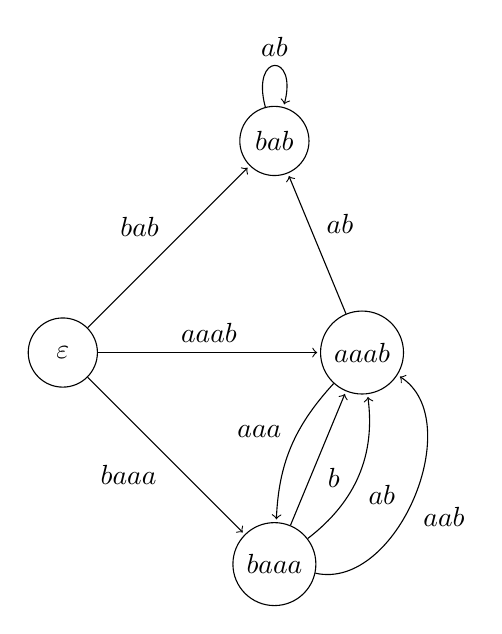
\begin{tikzpicture}[shorten >=1pt,node distance=3.8cm,on grid,auto]
	
   \node[state] (q_0)   {$\varepsilon$}; 
   \node[state] (q_1) [above right=of q_0] {$bab$}; 
   \node[state] (q_2) [below right=of q_0] {$baaa$}; 
   \node[state](q_3) [right=of q_0] {$aaab$};
    \path[->] 
    (q_0) edge  node {$bab$} (q_1)
          edge  node [swap] {$baaa$} (q_2)
          edge  node {$aaab$} (q_3)
    (q_1) edge [loop above] node {$ab$} ()
    (q_2) edge node [swap] {$b$} (q_3)
          edge [bend right=30] node [swap] {$ab$} (q_3)
          edge [bend right=80] node [swap] {$aab$} (q_3)
    (q_3) edge node [swap] {$ab$} (q_1)
          edge [bend right=20] node [swap]  {$aaa$} (q_2);
\end{tikzpicture}
\end{figure}

\begin{defn}[Walk in graph]
Let $G=(V,E,\phi,w)$ be a weighted digraph. A {\em walk} $W$ in $G$ of length $n$, $n \geq 1$ starting from $u$ and ending at $v$ is a sequence of the form $(e_1,e_2,\ldots,e_n)$, where $int(e_1)=u, fin(e_i) = int(e_{i+1})$ for all $i \in [n-1]$ and $fin(e_n)=v$. A walk is called $closed$ if $u=v$.

The weight of the walk $W$ is defined as the product of the weights of it's edges i.e., equal the word
\[w(W)=w(e_1) w(e_2) \cdots w(e_n)\]
\end{defn}

%\begin{remark}
%Note that the weight of a walk $W=(e_1,e_2,\ldots,e_n)$ in the correlation %graph $\mathbb{G}$ is the word $w(W)=w(e_1) w(e_2) \cdots w(e_n)$ where each %$w(e_1)$ belongs to the 
%\end{remark}

\begin{defn}[Adjacency matrix of a weighted digraph]
For every weighted digraph $G = (V, E, \phi, w)$ we define the matrix $A = [A_{ij}]$, of dimensions $|V| \times |V|$ as follows: $A_{ij}$ is the formal sum of 
\[A_{ij}=\sum_e w(e)\] 
where the sum is over every edge $e$ starting from $v_i$ and ending at $v_j$. The matrix $A$ is called the $adjacency$ $matrix$ of $G$ with respect to the weight function $w$.
\end{defn}

\noindent In order to have properly defined the adjacency matrix and the weight of a path on a digraph weighted with words, we need the following two operations between two words $w_1, w_2$:

\begin{enumerate}[label=\roman{*})]
\item A commutative formal sum of $w_1$ and $w_2$ which is noted as $w_1 + w_2$ where $\varepsilon$ is the identity element.

\item A non-commutative product which actually is the concatenation of $w_1$ and $w_2$ noted as $w_1 w_2$ where $\varepsilon w_1 = w_1 \varepsilon = \varepsilon$.
\end{enumerate}


\noindent Now, the matrix representation of $\mathbb{G}$ regarding the words $\tau_1,\tau_2,\ldots,\tau_r$ is the adjacency matrix $\mathbb{A}$:
\[\mathbb{A}= \begin{bmatrix}
	\varepsilon & \tau_1 & \tau_2 & \tau_3 & \ldots & \tau_r \\
    \varepsilon & {\mathcal{C}_{\tau_1,\tau_1}}^{\prime} & {\mathcal{C}_{\tau_1,\tau_2}}^{\prime} & {\mathcal{C}_{\tau_1,\tau_3}}^{\prime} & \dots  & {\mathcal{C}_{\tau_1,\tau_r}}^{\prime} \\
    \varepsilon & {\mathcal{C}_{\tau_2,\tau_1}}^{\prime} & {\mathcal{C}_{\tau_2,\tau_2}}^{\prime} & {\mathcal{C}_{\tau_2,\tau_3}}^{\prime} & \dots  & {\mathcal{C}_{\tau_2,\tau_r}}^{\prime} \\
    \vdots & \vdots & \vdots & \vdots & \ddots & \vdots \\
    \varepsilon & {\mathcal{C}_{\tau_r,\tau_1}}^{\prime} & {\mathcal{C}_{\tau_r,\tau_2}}^{\prime} & {\mathcal{C}_{\tau_r,\tau_3}}^{\prime} & \dots  & {\mathcal{C}_{\tau_r,\tau_r}}^{\prime}
\end{bmatrix}\]

where ${\mathcal{C}_{\tau_i,\tau_j}}^{\prime}= \sum\limits_{u \in \mathcal{C}_{\tau_i,\tau_j} } u $.
\begin{exa} Following the previous example, we have:
\[\mathbb{A}= \begin{bmatrix}
	\varepsilon & aaab & baaa & bab \\
    \varepsilon & \varepsilon & aaa & ab \\
    \varepsilon & b+ab+aab & \varepsilon & \varepsilon \\
    \varepsilon & \varepsilon & \varepsilon & ab
\end{bmatrix}\]
\end{exa}

\noindent We also denote as \[A_{ij}(n)=\sum_W w(W)\] the sum of the weights of all walks of length $n$ starting from the vertex $v_i$ and ending at the vertex $v_j$. This notation will be useful in proving the transfer-matrix method.

\noindent It is trivial that $A_{ij}=A_{ij}(1)$.

\section{The Transfer-Matrix Method}


\begin{prop}[Transfer-Matrix Theorem]
Let $A$ be the adjacency matrix of the weighted digraph $G=(V,E,\phi,w)$ and let $v_i, v_j$ be two vertices of $G$. The sum of the weights for all walks of length $n,n\geq1$ from $v_i$ to $v_j$ is equal to the $(i,j)$ element of the matrix $A^n$.
\end{prop}
\begin{proof}
We will use induction on $n$: \\
Base case: For $n=1$ the proposition holds by the definition of $A_{ij}$\\
Inductive hypothesis: Assume that the proposition holds for all values of $n$ up to some $k, k > 0$.\\
Inductive step: for $n=k+1$: \[(A^{k+1})_{ij}=(A^kA)_{ij}=\sum\limits_{\lambda = 1}^{|V|} (A^k)_{i \lambda } A_{\lambda j}\]
From the inductive hypothesis the term $(A^k)_{i \lambda }$ is the sum of weights for all walks of length $k$ which start from $v_i$ and end in $v_{\lambda}$. Furthermore, $A_{\lambda j}$ is the sum of weights for all edges $e$ ( or walks of length 1) with $int(e) = v_{\lambda}$ and $fin(e)=v_j$. Thus, $(A^k)_{i \lambda } A_{\lambda j}$ is the sum of weights for all walks of length $k+1$ which start from $v_i$ and reach $v_{\lambda}$ right before ending in $v_j$. This leads to $\sum\limits_{\lambda = 1}^{|V|} (A^k)_{i \lambda } A_{\lambda j}$ being the sum of weights for all paths of length $k+1$ which start from $v_i$ and end in $v_j$ with next to last vertex any $v \in V$. Implying, it is indeed the sum of weights for all paths of length $k+1$ which start from $v_i$ and end in $v_j$.
\end{proof}

\begin{exa} Consider the following graph $G$:
\end{exa}

\begin{figure}[ht]\centering
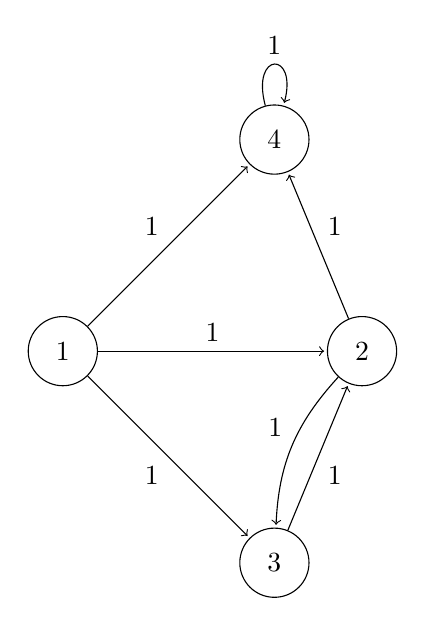
\begin{tikzpicture}[shorten >=1pt,node distance=3.8cm,on grid,auto]
	
   \node[state] (q_0)   {1}; 
   \node[state] (q_1) [above right=of q_0] {4}; 
   \node[state] (q_2) [below right=of q_0] {3}; 
   \node[state](q_3) [right=of q_0] {2};
    \path[->] 
    (q_0) edge  node {1} (q_1)
          edge  node [swap] {1} (q_2)
          edge  node {1} (q_3)
    (q_1) edge [loop above] node {1} ()
    (q_2) edge node [swap] {1} (q_3)
    (q_3) edge node [swap] {1} (q_1)
          edge [bend right=20] node [swap]  {1} (q_2);
\end{tikzpicture}
\end{figure}

\noindent The adjacency matrix $A$ of $G$ is:

\[A= \begin{bmatrix}
	0 & 1 & 1 & 1 \\
    0 & 0 & 1 & 1 \\
    0 & 1 & 0 & 0 \\
    0 & 0 & 0 & 1
\end{bmatrix}\]

and 

\[A^4= \begin{bmatrix}
	0 & 1 & 1 & 4 \\
    0 & 1 & 0 & 2 \\
    0 & 0 & 1 & 2 \\
    0 & 0 & 0 & 1
\end{bmatrix}\]

\noindent The transfer-matrix theorem states that since $a_{1,4} = 4$, there are four paths of length 4 starting from $1$ and ending in $4$. These are: $(1,4,4,4,4),(1,2,4,4,4),(1,2,3,2,4),(1,3,2,4,4)$.

\begin{prop} $det(I-xA)$ is invertible for every $A \in M$ such that $det(I-xA) \in R[[x]]$, where $R[[x]]$ is the ring of formal power series.
\end{prop}

\begin{proof}
It is well known that a formal series is invertible if and only if it has a nonzero constant term. Therefore:
\begin{align*}
det(I-xA) &= det(I-\frac{1}{z} A)  \\
&= det(\frac{1}{z}(zI-A))  \\
&= (\frac{1}{z})^n det(zI-A) \\
&= \frac{(-1)^n}{z^n} det(A-zI) \\
&= \frac{(-1)^n}{z^n} ((-1)^n z^n + b_{n-1} z^{n-1} + \ldots + b_1 z + b_0 ) \\
&= 1 + (-1)^n (b_{n-1} z^{-1} + \ldots + b_1 z^{-(n-1)} + b_0 z^{-n} ) \\
&= 1 + (-1)^n (b_{n-1} x + \ldots + b_1 x^{n-1} + b_0 x^n )
\end{align*}
where $b_0,b_1,\ldots,b_n \in R$.
\end{proof}

\begin{prop}
$\sum\limits_{n=0} A^n x^n = (I-xA)^{-1}$ where $I-xA, \sum\limits_{n=0} A^n x^n \in M[[x]]$, where $M$ is the set of all $m \times m$ matrices.
\end{prop}

\begin{proof}
\begin{align*}
[x^n](I-xA) \sum\limits_{j=0} A^j x^j &= \sum\limits_{k=0}^n [x^k] (I-xA) [x^{n-k}] \sum\limits_{j=0} A^j x^j \\
&= \begin{cases} I A^0, & n=0 \\
I A^n + (-A) A^{n-1}, & n\geq 1 \end{cases} \\
&= \begin{cases} I, & n=0 \\
0, & n\geq 1 \end{cases}
\end{align*}
\end{proof}

\begin{cor}
It follows from the previous proposition that if $(A)_{ij}$ is the $i,j$-th element of a matrix $A \in M$ then $(\sum\limits_{n=0} A^n x^n)_{ij}=((I-xA)^{-1})_{ij}$.
\end{cor}


\section{Generating Functions}
Generating functions are a very useful tool when solving enumeration problems. They can find an exact, recurrence or an asymptotic formula for non negative integer sequences as well as calculate mean averages, statistical properties and prove identities. The manipulation of generating functions is carried out in the ring of formal power series, hence there is no need to take matters of convergence into account. The theory of generating functions has been rigorously described in the books Generatingfunctionology (2005) \cite{W2005} of H. Wilf and Analytic Combinatorics(2013)\cite{FS2013} of P. Flajolet and R. Sedgewick. In the following, some notations are given about ordinary generating functions or simply generating functions.\\


\noindent There are two ways to define a generating function. The first is based on a non negative sequence $(a_n)$ such as:
\[F(x)=\sum\limits_{n=0}^\infty a_n x^n\]

\noindent For the second approach, let $S$ be a combinatorial class. Every function $p : S \to \mathbb{N}$ is called {\em parameter} and the generating function of $S$ respecting the parameter $p$ is defined as:
\[F(x)=\sum\limits_{a\in S} x^{p(\alpha)}\]

\begin{remark}The parameter $p$ can partition $S$ into the sets $S_n,n\in \mathbb{N}$ where:
\[S_n=\{\alpha \in S: p(\alpha)=n\}\]
\end{remark}
\noindent These two approaches are equivalent if we let $a_n$ be the cardinality of $S_n$.

\noindent Indeed,
\[ \sum\limits_{\alpha \in S} x^{p(\alpha)} = \sum\limits_{n \in \mathbb{N}} \sum\limits_{\alpha \in S_n} x^{p(a)} = 
\sum\limits_{n \in \mathbb{N}} \sum\limits_{\alpha \in S_n} x^n = \sum\limits_{n \in \mathbb{N}} x^n \sum\limits_{\alpha \in S_n} 1 =
\sum\limits_{n \in \mathbb{N}} |S_n| x^n \]

\noindent In other words, an ordinary generating function $F(x)$ is a formal power series with respect to the variable $x$, in which the coefficient of $x^n$ denoted as $[x^n]F(x)$ is the number of elements $\alpha$ in the set $S$ such that $p(\alpha)=n$.\\

\noindent The bivariate generating function of a sequence $(a_{n,k})$ is defined as:
\[F(x,y)=\sum\limits_{n=0}^\infty \sum\limits_{k=0}^\infty a_{n,k} x^n y^k\]

\noindent Equivalently, the bivariate generating function of $S$ with respect to the parameters $p,q: S \to \mathbb{N}$ is defined as:
\[F(x,y)=\sum\limits_{\alpha \in S} x^{p(\alpha)} y^{q(\alpha)}\]

\noindent and the coefficient of $x^n y^k$ is denoted as $[x^n y^k]F(x,y)]$. 

\noindent Multivariate generating functions with more than two variables are defined in a similar way. 



\subsubsection{Combinatorial Interpretations}


\noindent Let $F(x,y)$ be the generating function of $S$ with respect to the parameters $p,q$.

\begin{enumerate}[label=\roman{*})]

\item Let $y=1$, then the generating function $F(x,1)=F(x)$ enumerates the elements of $S$ based on solely the parameter $p$.

\item Let $y=0$, then the generating function $F(x,0)$ enumerates the elements of $S$ whose image of the parameter $q$ is $0$ regarding the parameter $p$. 

\item $\frac{[x^n] \frac{\partial F}{ \partial y} \big\vert_{y=1}}{[x^n]F(x,1)}$ Is the (mean) average number of objects regarding the parameter $q$, where their image of the parameter $p$ is $n$.

In general, the mean average of a variable $X$, which consists of the values $x_1,x_2,\ldots,x_k$ as well as their respective frequencies $n_1, n_2,\ldots,n_k$, is denoted by: \[\mu = \frac{\sum\limits_{i=1}^k x_i n_i}{\sum\limits_{i=1}^k n_i}\] 
Indeed, in the case of a bivariate generating function:

\begin{align*}
\frac{\partial F}{ \partial y}
	&= \sum\limits_{n=0}\sum\limits_{k=0} k a_{n,k} x^n y^{k-1} \\
	&= \sum\limits_{n=0}\sum\limits_{k=1} k a_{n,k} x^n y^{k-1}
\end{align*}
\begin{align*}
\frac{\partial F}{ \partial y} \bigg\vert_{y=1}
&= \sum\limits_{n=0}\sum\limits_{k=1} k a_{n,k} x^n
\end{align*}
Clearly, $[x^n]=\sum\limits_{k=1} k a_{n,k}= a_{n,1} + 2a_{n,2} + \ldots + m a_{n,m}$. The $k a_{n,k}$ term means that $k$ objects are accounted for every object with the image of the first parameter equal to $n$ and equivalently the second's equal to $k$. Thus, dividing by $[x^n] F(x,1)$ which is the count of all objects with the image of the first parameter equal to $n$ leads to: \[\mu(n)=\frac{a_{n,1} + 2a_{n,2}+3a_{n,3} + \ldots + m a_{n,m}}{a_{n,0}+a_{n,1} + a_{n,2}+a_{n,3} + \ldots + a_{n,m}}=\frac{\sum\limits_{k=1}^m k a_{n,k}}{\sum\limits_{k=0}^m a_{n,k}}\]

\begin{remark} In the case of strings, it is well known that the amount of words of length $n$ in a finite alphabet $A$ will be $|A|^n$. Therefore, substituting $x$ with $\frac{x}{|A|}$ in $ \frac{\partial F}{ \partial y} \vert_{y=1}$ will make it equal to $\mu(n)$ as well.
\end{remark}

\item The coefficients of a generating function can easily be evaluated using the Taylor theorem which states that a function $f: \mathbb{R} \rightarrow \mathbb{R}$ which is $k \in \mathbb{N^*}$ times differentiable at the point $x_0 \in \mathbb{R}$ is approximated by:
\[f(x)=\sum\limits_{n=0}^k \frac{f^{(k)}(x_0)}{n!}(x-x_0)^n + R_{k,f,x_0}(x)\]
where $R_{k,f,x_0}$ is the remainder.
\end{enumerate}

\noindent The usefulness of these interpretations can be seen in the last chapter when it comes to solving problems. Regarding the Taylor theorem, in our cases the generating functions are rational and with constant term $\pm 1$ in the denominator, thus they are infinitely differentiable at $x_0 = 0$ and as $k\rightarrow \infty : R_{k,f,0}\rightarrow 0$. Applying this in Python's sage is as easy as:

{{\setstretch{1.0}
\begin{lstlisting}{Sage}[]{language=Python}
sage: G(x)=-(x^7 - x^6 + x^5 - 5*x^4 - 7*x^3 + x^2 + 5*x + 1)/
(x^9 - x^8 - 2*x^6 - 10*x^5 + 4*x^4 + 2*x^3 + 3*x - 1)
sage: G.series(x,16)
x |--> 1 + 8*x + 25*x^2 + 70*x^3 + 225*x^4 + 748*x^5 + 2401*x^6 
+ 7668*x^7 + 24649*x^8 + 79344*x^9 + 255025*x^10 + 819494*x^11 
+ 2634129*x^12 + 8467464*x^13 + 27217089*x^14 + 87483296*x^15 
+ Order(x^16)
\end{lstlisting}
}

\chapter{The Goulden-Jackson cluster method}

\section{Historical review}

Some of the problems that showed up after the rise of the computer science in the previous decades was of the kind: How many binary words of length $n$ include the binary word $101$ and how many times does it occur in each word. To solve this problem of enumeration with generating functions one needs to consider that each binary word can be partioned as the empty word $\varepsilon$, a binary word starting with $1$ or a binary word starting with $0$ and then act as follows:

\begin{align*}
F(x,y)=\sum\limits_{a \in A^*} x^{|a|} y^{{|a|}_{101}} &= 1 + \sum\limits_{a \in A^*} x^{|1a|} y^{{|1a|}_{101}} + \sum\limits_{a \in A^*} x^{|0a|} y^{{|0a|}_{101}} \\
&= 1 + x \sum\limits_{a \in A^*} x^{|a|} y^{{|1a|}_{101}} + xF(x,y) \\
&= 1 + xF(x,y) + x \big( 1 + \sum\limits_{a \in A^*} x^{|1a|} y^{{|11a|}_{101}} + \sum\limits_{a \in A^*} x^{|0a|} y^{{|10a|}_{101}} \big) \\
&= 1 + xF(x,y) + x \big( 1 + xF(x,y) + x\sum\limits_{a \in A^*} x^{|a|} y^{{|10a|}_{101}} \big) \\
&= 1 + x + ( x + x^2 )F(x,y) + x^2 \sum\limits_{a \in A^*} x^{|a|} y^{{|10a|}_{101}} \\
&= 1 + x + ( x + x^2 )F(x,y) \\
&+ x^2 \big( 1 + \sum\limits_{a \in A^*} x^{|1a|} y^{{|101a|}_{101}}  + \sum\limits_{a \in A^*} x^{|0a|} y^{{|100a|}_{101}}   \big) \\
&= 1 + x + ( x + x^2)F(x,y) + x^2 + x^3 y F(x,y) + x^3 F(x,y) \\
&= 1 + x + x^2 + ( x + x^2 + x^3 + x^3 y )F(x,y) 
\end{align*}
\[
F(x,y)= \sum\limits_{a \in A^*} x^{|a|} y^{{|a|}_{101}} =\frac{ 1 + x + x^2 }{ 1 - x -x^2 -x^3 -x^3 y}
\]

This, however, requires a lot of algebraic manipulation with an alphabet of only two letters and a pattern of length 2. To solve harder problems than this where the alphabet has many letters and the problem requires counting occurences of more than two patterns simultaneously, one more powerful tool is required. This is exactly what the Goulden-Jackson cluster method (GJCM) does.

The GJCM was introduced By I.P. Goulden and D.M. Jackson (1979) in \cite{GJ1979},\cite{GJ1983} as a general method to count the number of words of $L^*$ avoiding patterns from a prescribed set. Two years later the notion of the autocorrelation of a word which is extended to correlation between words is introduced by L.J. Guibas and A.M. Odlyzko (1981) in \cite{GO1981},\cite{GO21981}, a notion that is also described in this thesis. In contrast to Goulden and Jackson (1979)\cite{GJ1979}, Guibas and Odlyzko (1981)\cite{GO1981},\cite{GO21981} worked with specific cases such as: enumerating sequences avoiding a pattern or sequences ending with the first occurence of a pattern. Later, M.Régnier and Szpankowski (1997) \cite{RS1997} used multivariate analysis to count several words simultaneously. A year later they applied their previous work to markovian sequences (1998)\cite{RS1998}. The method that was formally introduced by Goulden and Jackson (1979)\cite{GJ1979} was about the reduced case where the patterns do not occur in each other. Almost twenty years after that, J. Noonan and D. Zeilberger (1999) \cite{NZ1999} solved the problem of the non-reduced case, but without publishing an explicit formula. They provided, however, a sparse linear system as a solution along with the maple packages that solve it. This generalization was made in order to enumerate the words of $L^*$ with a fixed number of occurrences of patterns from a prescribed set. Six years after that, along with the relevant book of M. Lothaire {\em Applied Combinatorics on Words} (2005) \cite{L2005}, Y. Kong applied the method to an assymetrical Bernoulli model that is used to generate symbols (2005)\cite{K2005}. His work was based on the results of Noonan and Zeilberger (1999) \cite{NZ1999} for the reduced case.
Kong also emphasized on the idea of Goulden and Jackson \cite{GJ1979},\cite{GJ1983} about the inclusion-exclusion approach for its simplicity, while comparing it to the Régnier and Szpankowski method \cite{RS1997}. Following up, alternative proofs for both the reduced and non-reduced cases were given by F. Bassino, J. Clément, et al. (2007) \cite{BCFN2007}. In a newer version of their paper they provided a new approach with the use of Automata (2012)\cite{BCN2012} and more specifically based on the Aho-Corasick Automaton (1975) \cite{AC1975}. In all the above cases the enumerations were made possible by using generating functions. It is worth mentioning that some applications of the GJCM in biology and more specifically in genomes were made by B. Hao, et al. (2000)\cite{H2000}, \cite{HXYC2000}, \cite{2HXYC2000} and (2002) \cite{XB2002}. A notable example is the creation of fractals based on the under or over representation of certain DNA strings and the use of the GJCM to evaluate the dimension of these fractals \cite{H2000}.


\section{Counting one pattern}

\noindent The case of counting words with one pattern is interesting in its own and will give a nice introduction to the GJCM.

\subsection{Marked words}

The occurrences of the pattern $\tau$ in $w$ can be encoded by the elements of the set
\[ S_\tau(w) = \{i \in [n]: \tau \textrm{ starts at the $i$-th position of $w$}\}, \]
that is, each element of $S_\tau(w)$ indicates the position of the first letter of an occurrence of $\tau$ in $w$. Clearly, $S_\tau(\varepsilon) = \varnothing$.

\begin{defn}[Marked Word]
A {\em marked word} is a pair $(w, I)$, where $w$ is a word and $I \subseteq S_\tau(w)$. An occurrence of $\tau$, starting at the $i$-th position of $w$, is {\em marked} in $(w, I)$ iff $i \in I$. Practically, a marked word is a word $w$ having some of its occurrences of $\tau$ marked. These markings are encoded by the set $I$.
\end{defn}

For example, let $\tau = aba$ be a pattern and $w=abaaaba$ be a word. Then $(w,\{5\})$ is a marked word.

Clearly, the word $w$ generates $2^{|w|_\tau}$ marked words, where $\binom{|w|_\tau}{k}$ of them have exactly $k$ markings. Every word $w$ can be considered to be marked, via the mapping $w \mapsto (w, \varnothing)$.

The concatenation of two marked words $(w, I)$, $(v, J)$ is defined as follows:
\[ (w, I)(v, J) = (wv, I \cup (|w| + J)). \]
where $|w| + J = \{|w| + j: j \in J\}$.

We denote by $MW$ the set of marked words, and we define
\[ H = H(x,y) = \sum\limits_{(w,I) \in MW} x^{|w|} y^{|I|} \]
to be its generating function, with respect to the length $|w|$ and the number of marked occurrences of $\tau$. 

The introduction of the set of marked words and its corresponding generating function $H$ is justified by the following proposition. 

\begin{prop}
Let $F = F(x,y) = \sum\limits_{w \in L^*} x^{|w|} y^{|w|_\tau}$ be the generating function of $L^*$ which counts the occurrences of the pattern $\tau$ and $H = H(x,y) = \sum\limits_{(w, I) \in MW} x^{|w|} y^{|I|}$ be the generating function of the set of marked words which counts the marked occurrences of $\tau$. Then
\[ H(x,y) = F(x, y+1). \]  
\end{prop}

\begin{proof} Indeed,
\begin{align*}
F(x,y+1) 
& = \sum\limits_{w \in L^*} x^{|w|} (y + 1)^{|w|_\tau} \\
& = \sum\limits_{w \in L^*} x^{|w|} \sum\limits_{k=0}^{|w|_\tau} \binom{|w|_\tau}{k} y^k \\
& = \sum\limits_{w \in L^*} x^{|w|} \sum\limits_{I \subseteq S_\tau(w)} y^{|I|}\\
& = \sum\limits_{(w, I) \in MW} x^{|w|} y^{|I|} \\
& = H(x,y)  \qedhere
\end{align*}
\end{proof}


\subsection{Clusters}

It turns out that evaluation of $H$ is much more straight-forward than the evaluation of $F$ but we need the notion of cluster.

\begin{defn}[Cluster]
 We recall that a {\em cluster} (of $\tau$) is a marked word that is not a concatenation of two marked words. Equivalenty, a cluster is a marked word $(c, I)$ satisfying the following two conditions:

\begin{enumerate}[label=\roman{*})]

\item Every letter in $c$ belongs to some marked occurrence of $\tau$.

\item Any two consecutive marked occurrences of $\tau$ in the cluster overlap.

\end{enumerate}
\end{defn}


\noindent Note that a cluster may contain occurrences of $\tau$ which are not marked.

For example, let $\tau=ababa$ be a pattern and $c = ababababa$ be a word. Then $(c,\{1,5\})$ is a cluster.
Note that, there is an occurrence of $\tau$ starting at the 3rd position of $c$ which is not marked.

We remark that $(c, I)$ is a cluster iff it satisfies the following conditions
\[ \min I = 1, \max I = |c| - |\tau| + 1\]
and the absolute differrence of any two consecutive elements of $I$ is less than $|\tau|$.

\begin{defn}[Set of Clusters]
We denote the set of all clusters of $\tau$ by $C_\tau$. The trivial cluster $(\tau, \{1\})$ of $C_\tau$ is denoted by $\tau$, for simplicity.
\end{defn}

\begin{defn}[Cluster Generating Function]
We define the generating function of the set of clusters $C_\tau$ for the pattern $\tau$ to be
\[ C(x,y) = \sum\limits_{(c,I) \in C_\tau} x^{|c|} y^{|I|} \]
\end{defn}

\noindent In order to evaluate $C$, we define the operation
\[ * : \mathcal{V}_\tau \times C_\tau \to C_\tau \setminus \{\tau \} \]
so that for a border $v \in \mathcal{V}_{\tau}$ and $(c^\prime, I^\prime) \in C_\tau$ we have:
\[ v * (c^\prime, I^\prime) = (l(v) c^\prime, I), \]
where $I = \{1\} \cup (|l(v)| + I^\prime)$. It is easy to check, using the definition of clusters, that $v * (c^\prime, I^\prime) \in C_\tau \setminus \{\tau\}$.

This operation can be used to decompose every element of $C_\tau \setminus \{\tau\}$. Indeed, if $(c, I) \in C_\tau \setminus \{\tau\}$, then the common segment $v$ of the first and second marked occurrence of $\tau$ in $(c,I)$ is a border of $\tau$. Setting $c = l(v) c^\prime$ and $I^\prime = -|l(v)| + (I \setminus \{1\})$, we obtain that
\[ (c,I) = v * (c^\prime, I^\prime). \]

\begin{prop} For every pattern $\tau \in L^*$ the cluster generating function of $MW$ is given by the formula
\[ C_\tau(x,y) = \frac{x^{|\tau|} y}{1 - x^{\tau} y \sum\limits_{v \in V_\tau} x^{-|v|}}.\]
\end{prop}

\begin{proof}
\begin{align*}
C_\tau(x,y) 
& = \sum\limits_{(c,I) \in C_\tau} x^{|c|} y^{|I|} \\
& = x^{|\tau|} y + \sum\limits_{v \in \mathcal{V}_\tau} \sum\limits_{(c^\prime I^\prime) \in C_\tau} x^{|l(v)|} x^{|c^\prime|} y^{|I^\prime|+1} \\
& = x^{|\tau|} y + y C_\tau(x,y) \sum\limits_{v \in \mathcal{V}_\tau} x^{|l(v)|}
\end{align*}
which leads to
\[ C_\tau(x,y) = \frac{x^{|\tau|} y}{1 - x^{|\tau|} y \sum\limits_{v \in V_\tau} x^{-|v|}}. \qedhere \]
\end{proof}

\noindent Now we have all the tools needed to evaluate $H(x,y)$. Every marked word can be decomposed uniquely as the concatenation of single letters which do not appear in any marked occurrence of $\tau$ and of clusters.

Every $(w, I) \in MW$ is uniquely decomposed as follows:
\[ (w, I) = \begin{cases} \varepsilon, \textrm{ or }\\
a (w^\prime, I^\prime), \textrm{ or } \\
(c, J) (w^\prime, I^\prime) 
\end{cases}\]
where $(c, J) \in C_{\tau}$, $(w^\prime, I^\prime) \in MW$ and $a \in L$.

\begin{prop} For every pattern $\tau \in L^*$ we have that:
\[ F(x,y) = \frac{1}{1 - x |L| - C_\tau(x,y-1)} \]
where 
\[ C_\tau(x,y) = \frac{x^{|\tau|} y}{1 - x^{|\tau|} y \sum\limits_{v \in V_\tau} x^{-|v|}}. \]
\end{prop}

\begin{proof}
\begin{align*}
H(x,y) 
& = \sum\limits_{(w, I) \in MW} x^{|w|} y^{|I|} \\
& = 1 + \sum\limits_{a \in L} \sum\limits_{(w^\prime, I^\prime) \in MW} x^{|w^\prime| + 1} y^{|I^\prime|} + \sum\limits_{(c, J) \in C_\tau} \sum\limits_{(w^\prime, I^\prime) \in MW} x^{|c| + |w^\prime|} y^{|J| + |I^\prime|} \\
& =  1 + x |L| H(x,y) + C_\tau(x,y) H(x,y)  
\end{align*}
hence we have that
\[ H(x,y) = \frac{1}{1 - x |L| - C_\tau(x,y)} \]
\end{proof}

\section{Counting multiple patterns - the reduced case}

\noindent We will now present how to count multiple patterns. For simplicity we consider the reduced case. The non-reduced case is more technical and is outside the scope of this thesis. In this case no pattern $\tau_j$ is a subword of another pattern $\tau_s$.
Essentialy, no marked occurrence is a factor of another marked occurrence.

\subsection{Marked words}

\noindent Now we need to distinguish each marked occurrence of a pattern individually. The occurrences of the patterns $\tau_1, \tau_2, \ldots, \tau_r$ in $w$ can be encoded by the elements of the sets
\[ S_{\tau_j}(w) = \{i \in [n]: \tau_j \textrm{ starts at the $i$-th position of $w$}\}, \]
that is, each element of $S_{\tau_j}(w)$ indicates the position of the first letter of an occurrence of $\tau_j$ in $w$. Clearly, $S_{\tau_j}(\varepsilon) = \varnothing$.
\begin{defn}[Marked Word]
A {\em marked word} is a (r+1)-tuple $(w, I_1, I_2, \ldots, I_r)$, where $w$ is a word and $I_j \subseteq S_{\tau_j}(w)$, $j \in [r]$. An occurrence of $\tau_j$, starting at the $i$-th position of $w$, is {\em marked} in $(w, I_1, I_2, \ldots, I_r)$ iff $i \in I_j$. Practically, a marked word is a word $w$ having some of its occurrences of $\tau_1, \tau_2, \ldots, \tau_r$ marked. These markings are encoded by the sets $I_1, I_2, \ldots, I_r$.
\end{defn}

For example, let $\tau_1= aab$ and $\tau_2=baa$ be two patterns and $w=aaabaaaab$ be a word. Then $(w,\{7\},\{4\})$ is a marked word ( of $\tau_1,\tau_2$ ).

Clearly, the word $w$ generates $2^{\sum\limits_{j=1}^r |w|_{\tau_j}}$ marked words, where $\binom{\sum\limits_{j=1}^r |w|_{\tau_j}}{k}$ of them have exactly $k$ markings. Every word $w$ can be considered to be marked, via the mapping $w \mapsto (w, \varnothing, \varnothing, \ldots, \varnothing)$.

The concatenation of two marked words $(w, I_1, I_2, \ldots, I_r)$, $(v, J_1, J_2, \ldots, J_r)$ is defined as follows:
\[ (w, I_1, I_2, \ldots, I_r)(v, J_1, J_2, \ldots, J_r) = (wv, I_1 \cup (|w| + J_1), I_2 \cup (|w| + J_2), \ldots, I_r \cup (|w| + J_r)). \]
where $|w| + J = \{|w| + j: j \in J\}$.


We denote by $MW$ the set of marked words, and we define
\[ H = H(x,y_1, y_2, \ldots, y_r) = \sum\limits_{(w,I_1, I_2, \ldots, I_r) \in MW} x^{|w|} y^{|I_1|} y^{|I_2|} \cdots y^{|I_r|} = \sum\limits_{(w,I_1, I_2, \ldots, I_r) \in MW} x^{|w|} \prod\limits_{j=1}^r y^{|I_j|} \]
to be its generating function, with respect to the length $|w|$ and the number of marked occurrences of $\tau_1, \tau_2, \ldots, \tau_r$. 

\begin{prop}
Let $F = F(x,y_1, y_2, \ldots, y_r) = \sum\limits_{w \in L^*} x^{|w|} \prod\limits_{j=1}^r y_j^{|w|_{\tau_j}}$ be the generating function of $L^*$ which counts the occurrences of the pattern $\tau_1, \tau_2, \ldots, \tau_r$ and $H = H(x,y_1, y_2, \ldots, y_r) = \sum\limits_{(w, I_1, I_2, \ldots, I_r) \in MW} x^{|w|} \prod\limits_{j=1}^r y_j^{|I_j|}$ be the generating function of the set of marked words which counts the marked occurrences of $\tau_1, \tau_2, \ldots, \tau_r$. Then
\[ H(x,y_1, y_2, \ldots, y_r) = F(x, y_1+1, y_2+1, \ldots, y_r+1). \]  
\end{prop}

\begin{proof} Indeed,
\begin{align*}
F(x,y_1+1, y_2+1,\ldots, y_r+1) 
& = \sum\limits_{w \in L^*} x^{|w|} \prod\limits_{j=1}^r (y_j + 1)^{|w|_{\tau_j}} \\
& = \sum\limits_{w \in L^*} x^{|w|} \prod\limits_{j=1}^r \sum\limits_{k=0}^{|w|_{\tau_j}} \binom{|w|_{\tau_j}}{k} y_j^k \\
& = \sum\limits_{w \in L^*} x^{|w|} \prod\limits_{j=1}^r \sum\limits_{I_j \subseteq S_{\tau_j}(w)} y_j^{|I_j|}\\
& = \sum\limits_{(w, I_1, I_2, \ldots I_r) \in MW} x^{|w|} \prod\limits_{j=1}^r y_j^{|I_j|} \\
& = H(x,y_1, y_2, \ldots, y_r)  \qedhere
\end{align*}
\end{proof}


\subsection{Clusters}

For the evaluation of $H$ we need to generalize the notion of cluster. 

A {\em cluster} (of $\tau_1, \tau_2, \ldots, \tau_r$) is a marked word that is not a concatenation of two marked words. Equivalenty, a cluster is a marked word $(c, I_1, I_2, \ldots, I_r)$ satisfying the following two conditions:

\begin{enumerate}[label=\roman{*})]

\item Every letter in $c$ belongs to some marked occurrence of $\tau_1, \tau_2, \ldots, \tau_r$.

\item Any two consecutive marked occurrences of $\tau_i$, $\tau_j$ in the cluster overlap.

\end{enumerate}

Note that a cluster may contain occurrences of $\tau_j$'s which are not marked.

For example, let $\tau_1 = ababa$ and $\tau_2=babab$ be two patterns and $c = ababababababa$ be a word. Then $(c,\{1,9\},\{4,8\})$ is a cluster. Note that, there are occurrences starting at the 2nd and 3rd position of $c$ which are not marked.

We remark that $(c, I_1, I_2, \ldots, I_r)$ is a cluster iff it satisfies the following conditions:
\[ \min \bigcup\limits_{j=1}^r I_j = 1, \max \bigcup\limits_{j=1}^r I_j = |c| - |\tau_s| + 1, \textrm{ for some $\tau_s$, $s \in [r]$.}  \]
and the absolute differrence of any two consecutive elements $p, q$ of $\bigcup\limits_{j=1}^r I_j$ is less than $|\tau_s|$ whenever $p \in I_s$.

We denote the set of all clusters of $\tau_1, \tau_2, \ldots, \tau_r$ by $C_{\tau_1, \tau_2, \ldots, \tau_r}$. 

The trivial clusters $(\tau_j,\varnothing, \ldots, \varnothing, \underbrace{\{1\}}_{\textrm{$j$-th position}}, \varnothing, \ldots, \varnothing)$ of $C_{\tau_1, \tau_2, \ldots, \tau_r}$ are denoted by $\tau_j$, for simplicity.

The set $C_{\tau_1, \tau_2, \ldots, \tau_r}$ is partitioned into $r$ subsets where $I_j$ contains $1$. The set of clusters where $1 \in I_j$ is denoted by $C_{\tau_1, \tau_2, \ldots, \tau_r}^{\tau_j}$.

We define the generating function of the set of clusters $C_\tau$ for the pattern $\tau$ to be
\[ C(x,y_1, y_2, \ldots, y_r) = \sum\limits_{(c,I_1, I_2, \ldots, I_r) \in C_{\tau_1, \tau_2, \ldots, \tau_r}} x^{|c|} \prod\limits_{j=1}^r y_j^{|I_j|} \]

%Furthermore, we define the operations
%\[ * : \mathcal{C}_{\tau_s, \tau_j} \times C^{\tau_j}_{\tau_1, \tau_2, \ldots, \tau_r} \to C^{\tau_s}_{\tau_1, \tau_2, \ldots, \tau_r} \setminus \{\tau_s \} \]
%so that for $u \in \mathcal{C}_{\tau_s, \tau_j}$ and $(c^\prime, I_1^\prime, I_2^\prime, \ldots, I_r^\prime) \in C_{\tau_1, \tau_2, \ldots, \tau_r}^{\tau_j}$ we have
%\[ u * (c^\prime, I_1^\prime, I_2^\prime, \ldots, I_r^\prime) = (u c^\prime, I_1, I_2, \ldots, I_r), \]
%where $I_s = \{1\} \cup (|u| + I_s^\prime)$ and $I_j = |u| + I_j^\prime$ for $j \ne s$. It is easy to check, using the definition of clusters, that $u * (c^\prime, I_1^\prime, I_2^\prime, \ldots, I_r^\prime) \in C^{\tau_s}_{\tau_1, \tau_2,\ldots, \tau_r} \setminus \{\tau_s\}$. If $\mathcal{C}_{\tau_s, \tau_j} = \varnothing$ then {\bf the mapping is defined to be the identity.}

Every marked word can be decomposed uniquely as the concatenation of single letters which do not appear in any marked occurrence of $\tau$ and of clusters.

Every $(w, I_1, I_2, \ldots, I_r) \in MW$ is uniquely decomposed as follows:
\[ (w, I_1, I_2, \ldots, I_r) = \begin{cases} \varepsilon, \textrm{ or }\\
a (w^\prime, I_1^\prime, I_2^\prime, \ldots, I_r^\prime), \textrm{ or } \\
(c, J_1, J_2, \ldots, J_r) (w^\prime, I_1^\prime, I_2^\prime, \ldots, I_r^\prime) 
\end{cases}\]
where $(c, J_1, J_2, \ldots, J_r) \in C_{\tau_1, \tau_2, \ldots \tau_r}$, $(w^\prime, I_1^\prime, I_2^\prime, \ldots, I_r^\prime) \in MW$ and $a \in L$.

\begin{prop}
\[ F(x,y_1,\ldots,y_r) = \frac{1}{1 - x |L| - C_\tau(x,y_1-1, y_2-1,\ldots, y_r-1)} \]
where 
\[ C_\tau (x,y_1, y_2, \ldots, y_r) = \sum\limits_{(c,I_1, I_2, \ldots, I_r) \in C_{\tau_1, \tau_2, \ldots, \tau_r}} x^{|c|} \prod\limits_{j=1}^r y_j^{|I_j|} \]
\end{prop}

\begin{proof}
\begin{align*}
H(x,y) 
& = \sum\limits_{(w, I_1, I_2, \ldots, I_r) \in MW} x^{|w|} \prod\limits_{j=1}^r y_j^{|I_j|} \\
& = 1 + \sum\limits_{a \in L} \sum\limits_{(w^\prime, I_1^\prime, I_2^\prime, \ldots, I_r^\prime) \in MW} x^{|w^\prime| + 1} \prod\limits_{j=1}^r y_j^{|I_j^\prime|} + \sum\limits_{(c, J_1, J_2, \ldots, J_r) \in C_{\tau_1, \tau_2, \ldots, \tau_r}} \sum\limits_{(w^\prime, I_1^\prime, I_2^\prime, \ldots, I_r^\prime) \in MW} x^{|c| + |w^\prime|} y^{|J| + |I^\prime|} \\
& =  1 + x |L| H(x,y_1, y_2, \ldots, y_r) + C_\tau(x,y_1, y_2, \ldots y_r) H(x,y_1, y_2, \ldots, y_r)  
\end{align*}
hence we have that
\[ H(x,y) = \frac{1}{1 - x |L| - C_\tau(x,y_1, y_2,\ldots, y_r)}. \qedhere \]
\end{proof}

\noindent In other words, the problem of evaluating $F$ is reduced to the problem of evaluating the cluster generating function for multiple patterns. This, however, is out of the scope of this dissertation. The purpose was to demonstrate the previous mathematical techniques regarding words and the inclusion-exclusion approach on how to count them. In the remaining part of this chapter we establish a bijection between clusters and weights of paths and then we state the main theorem.

\begin{comment}
In order to do this, the following notations are given:

\begin{enumerate}[label=\roman{*})]
\item For any set of patterns $T=\{\tau_1,\tau_2,\ldots,\tau_r\}$ a $(1\times r)$-vector is defined as $\overline{T}=[x^{|\tau_1|},x^{|\tau_2|},\ldots,x^{|\tau_r|}] $ where $x \in R$, $x$ is an indeterminate which counts the length of the corresponding pattern and $(R,+,\cdot)$ is a commutative ring. The vector $\overline{T} $ is called the {\em generating vector} of $T$.

\item Equivalently, given the adjacency matrix $\mathbb{A}=[a_{ij}]$ of the correlation graph $\mathbb{G}$ of $T$, the {\em generating matrix} of $\mathbb{A}$ is defined as $\overline{\mathbb{A}}=[\underline{a_{ij}}]$ where $\underline{a_{ij}}$ is the basic generating function of the set of words $a_{ij}$.

\item In order to count the marked occurrences of $T$, an $r \times r$ diagonal matrix is defined as: 
\[\Delta (T)=\begin{bmatrix}
    y_1 & 0 & 0 & \dots & 0 \\
    0 & y_2 & 0 & \dots  & 0 \\
    0 & 0 & y_3 & \dots  & 0 \\
    \vdots & \vdots & \vdots & \ddots & \vdots \\
    0 & 0 & 0 & \dots & y_r
\end{bmatrix} \]
where each $y_i \in R, \forall i\in [r]$ is an indeterminate which counts the marked occurrences of the pattern $\tau_i$ and $(R,+,\cdot)$ is a commutative ring.
\end{enumerate}
\end{comment}

\begin{prop} A marked word $(c,I_1,I_2,\ldots,I_r)$ (of $\tau_1, \tau_2, \ldots, \tau_r)$ is a cluster if and only if $c$ is the weight of a walk starting from $\varepsilon$ in the correlation graph $\mathbb{G}$ of $\tau_1, \tau_2, \ldots, \tau_r$.

%There exists a bijection between marked words
\end{prop}
\begin{proof}
Let $W$ be a walk in $\mathbb{G}$ starting from $\varepsilon$ with length $k$, i.e. \[W = \varepsilon \xrightarrow{e_0} v_0 \xrightarrow{e_1} v_1 \xrightarrow{e_2} v_2 \ldots \xrightarrow{e_k} v_k\]

Then, $v_0,v_1,v_2,\ldots,v_k \in T$, $w(e_0) \in T$ and $w(e_j) \in \mathcal{C}_{\tau_{j},\tau_{j-1}}$
We define a marked word $(w,I_1,I_2,\ldots,I_r)$ as follows:

$w=w(e_k)w(e_{k-1})\ldots w(e_2)w(e_1)$ and the sets $I_1,I_2,\ldots, I_r$ are defined inductively:

$I_1,I_2,\ldots,I_r=\varnothing$. For every edge $e_j$ set:

\begin{enumerate}[label=\roman{*})]

\item Increase all elements of $I_1, I_2,\ldots,I_r$ by $|w(e_j)|$ (if there are any).

\item Add 1 as a new element to the set $I_s$ where $fin(e_j)=v_j=\tau_s$.
\end{enumerate}

In other words, we start from a pattern and mark its occurrence, then we concatenate elements from the correlation sets creating new overlapping (by definition of correlation sets) occurrences. We mark these occurrences at the starting position of the new word $w(e_j)\ldots w(e_1) w(e_0)$ as well as shifting the previous marked occurrences to their new positions. As a consequence, any two consecutive marked occurrences overlap and every letter of $w(e_k) \ldots w(e_1) w(e_0)$ belongs in a correlation set or the starting pattern from which marked occurrences are created, implying it belongs in a marked occurrence. Hence $(w(e_k) \ldots w(e_1) w(e_0),I_1,I_2,\ldots,I_r)$ is a cluster.


%
%Let a walk $W$ in $\mathbb{G}$ be:
%\[\varepsilon \xrightarrow{e_0} v_0 \xrightarrow{e_1} v_1 \xrightarrow{e_2} v_2 \ldots \xrightarrow{e_k} v_k\]
%where $v_0,v_1,\ldots v_k \in V\setminus\{\varepsilon\}$ and $e_0,e_1,\ldots e_k \in E$ as well as $w(e_i) = y_i$. Furthermore, the weight of $W$ is $y_k \ldots y_1 y_0$. Since we are starting the walk $W$ from $\varepsilon$ we have $I_1,I_2,\ldots,I_r=\varnothing$ and while following it's edges, at every step $j$ we do the following:
%\begin{enumerate}[label=\roman{*})]
%
%\item Add $|y_j|$ to all elements of $I_1, I_2,\ldots,I_r$ (if there are any).
%
%\item Add 1 as a new element to the set $I_s$ where $fin(e_j)=v_j=\tau_s$.
%\end{enumerate}
%
%With this loop we start from a pattern and mark its occurrence, then we concatenate elements from the correlation sets creating new overlapping (by definition of correlation sets) occurrences. We mark these occurrences at the starting position of the new word $y_j\ldots y_1 y_0$ as well as shifting the previous marked occurrences to their new positions. As a consequence, any two consecutive marked occurrences overlap and every letter of $y_k \ldots y_1 y_0$ belongs in a correlation set or the starting pattern from which marked occurrences are created, implying it belongs in a marked occurrence. Hence $(y_k \ldots y_1 y_0,I_1,I_2,\ldots,I_r)$ is a cluster.

Conversely, let $(c,I_1,\ldots,I_r)$ be a cluster of $\tau_1, \tau_2,\ldots,\tau_r$.
We build a sequence of the form \\ $((v_1,p_1),(v_2,p_2),\ldots,(v_k,p_k))$ where $p_j$ is the starting position of the word $v_j$ (a pattern) in $c$. The sequence is sorted in descending order of the positions $p$ such as:
$p_1 = |c|-|v_1| + 1 > p_2 > \dots > p_k = 1$. Furthermore, let $w[m,n]$ be the subword which starts from the $m$-th position and ends at the $n$-th position of $c$. For example, if $c=aabaa$ then $w[3,5]= baa$. Each word $w[p_j,|c|]$ for all $j\in[k]$ is a suffix of $c$ and starts with a marked occurrence of a pattern. Therefore, all of it's letters belong in a marked occurrence and every two consecutive marked occurences overlap, as this happens by definition in $c$ and $w[p_j,|c|]$ can't contain the prefix of a marked occurrence without it's suffix. We set $y_1 = v_1$ and each $y_j$ is the word such that $y_j w[p_{j-1},|c|] = w[p_j,|c|]$, for all $j \in \{2,\ldots,k\}$. By definition of the correlation sets, $y_j \in \mathcal{C}_{v_j,v_{j-1}}$ for all $j \in \{2,\ldots,k\}$. This leads to a unique walk $c=y_k \ldots y_2 y_1$ of the graph $\mathbb{G}$ such as:
\[\varepsilon \xrightarrow{y_1} v_1 \xrightarrow{y_2} v_2 \xrightarrow{y_3} \ldots \xrightarrow{y_k} v_k\]
Hence there is a bijection mapping walks of $\mathbb{G}$ to clusters.
\end{proof}

\begin{prop}[Cluster Generating Function]

Let $T$ be a set of $r$ patterns and $\mathbb{A}$ the corresponding adjacency matrix. We use the transformation $\phi : \mathcal{C}_{\tau_i,\tau_j} \rightarrow R[x,y_j], \phi(u)= x^{|u|} y_j$ 
and map each element $a_{i,j}$ of $\mathbb{A}$ to $\phi(a_{i,j})$. This image will be the $i,j$-th element of a new matrix $\overline{\mathbb{A}}$. Then:

\[C_\tau (x,y_1,y_2,\ldots,y_r) = [1,0,0,\ldots,0] \quad (I - \overline{\mathbb{A}})^{-1}\quad \begin{bmatrix}
    1 \\
    1 \\
    \vdots \\
    1
\end{bmatrix} \]
\end{prop}

\begin{comment}
\begin{proof}
The set of clusters is decomposed either as the trivial clusters $\tau_s$ or the weights of walks on the corresponding correlation graph $\mathbb{G}$, as shown in the previous proposition. Furthermore, the sum regarding the weights of the walks on $\mathbb{G}$ with the second vertex visited being $\tau_i$ (the first is a trivial cluster $\tau_s$) and the ending vertex being $\tau_j$, with a total of $n+1$ marked occurrences from all the patterns combined, is $\tau_s * (i,j-$th element of $\mathbb{A}^n$). This is a consequence of proposition 5, in which case the length of the walk is the number of total marked occurrences (except for the first one).

\noindent Implying, the elements of the sets in the vector $[\tau_1,\tau_2,\ldots,\tau_r] * \sum\limits_{n=0} \mathbb{A}^n$ are the words from all the possible clusters. Thus, the set of the words from all clusters of $\tau_1,\tau_2,\ldots,\tau_r$ is:
\[[\tau_1,\tau_2,\ldots,\tau_r]* \mathbb{A}^* * \mathbb{E}\]
where $\mathbb{E}$ is the ($r\times 1$) vector $\begin{bmatrix}
    \varepsilon \\
    \varepsilon \\
    \vdots \\
    \varepsilon
\end{bmatrix}$\\


\noindent In order to count each marked occurrence and transition this set into the desired generating function, the following mappings are used as well as proposition 4:

\begin{enumerate}[label=\roman{*})]
\item The $*$ operation $\rightarrow$ the $\cdot$ operation.
\item $[\tau_1,\tau_2,\ldots,\tau_r] \rightarrow \overline{T} \Delta(T)$
\item $\mathbb{A} \rightarrow \overline{\mathbb{A}} \Delta(T)$
\item $\mathbb{E} \rightarrow \overline{\mathbb{E}}$
\end{enumerate}

\noindent All of which lead to:
\[C_\tau (x,y_1,\ldots,y_r) = \overline{T} \Delta(T) \cdot (I - \overline{\mathbb{A}} \Delta(T))^{-1} \cdot \begin{bmatrix}
    1 \\
    1 \\
    \vdots \\
    1
\end{bmatrix}\]

\end{proof}
\end{comment}

\begin{exa} Let $\tau_1 =aaab$ and $ \tau_2 = baaa$ in $\{a,b\}^*$. The adjacency matrix is:
\[\mathbb{A} = \begin{bmatrix}
	\varepsilon & aaab & baaa \\
    \varepsilon & \varepsilon & aaa \\
    \varepsilon & b+ba+baa & \varepsilon
\end{bmatrix}\]

Thus, the cluster generating function is:

\begin{align*}
C(x,y_1,y_2)
&= [1,0,0] \begin{bmatrix}
	1 & -x^4 y_1 & -x^4 y_2 \\
    0 & 1 & -x^3 y_2 \\
    0 &-(x+x^2 + x^3)y_1 & 1
\end{bmatrix}^{-1} \begin{bmatrix}
    1\\
    1\\
    1
\end{bmatrix}\\
&= \frac{x^4 y_1 + x^4 y_2 + x^7 y_1 y_2 + (x^5 + x^6 + x^7)y_1 y_2}{1-y_1 y_2 (x^4 + x^5 + x^6)}
\end{align*}
\end{exa}





\chapter{Applications of the Goulden-Jackson cluster method}

\noindent Using the GJCM we can evaluate the generating function for various sets of patterns.

\section{Different kinds of positions on $3 \times n$ Chessboards}

\noindent In this chapter, we consider a set of problems where we do not need to count words but formations on a $3\times n, n \in \mathbb{N}^*$ chessboard with various properties. By associating each column to a letter we can reduce the problem of counting proper formations to the problem of counting words avoiding specifics set of patterns. For all of these we use some Python scripts to find the correlation set and the correlation matrix and the program sage to perform the computations. Most of the corresponding generating functions' coefficients appear in OEIS but some of them are new.

\subsection{Non-Attacking Bishop positions}

In \cite{LK2017}, Low and Kapbasov evaluated the generating function which counts the number of non-attacking bishop positions on the $3 \times n$ chessboards. Using generating functions regarding black and white squares they provided the generating function: \[\mathbb{B}_3(x)=\frac{-1-5x-x^2+7x^3+5x^4-x^5+x^6-x^7}{-1+3x+2x^3+4x^4-10x^5-2x^6-x^8+x^9}\]

However, they provided the idea of associating the $2^3$ bishop positions with letters such as: \\

\tikzset{node distance = 0.55cm and 2cm}
\tikzstyle{box} = [rectangle, draw, black]

\begin{figure}[ht]
        \centering
        \begin{subfigure}[b]{0.1\textwidth}
                \centering

\begin{tikzpicture}
\node (first) [box,,minimum size=0.57cm] {};
\node (second) [box,below of=first,minimum size=0.57cm] {};
\node (third) [box,below of=second,minimum size=0.57cm] {};
\node (fourth) [below of=third,] {0};
\draw (first)(second)(third)(fourth);
\end{tikzpicture}
\end{subfigure}\begin{subfigure}[b]{0.1\textwidth}
        	\centering

\begin{tikzpicture}
\node (first) [box,minimum size=0.57cm] {};
\node (second) [box,below of=first,minimum size=0.57cm] {};
\node (third) [box,below of=second,minimum size=0.57cm] {B};
\node (fourth) [below of=third] {1};
\draw (first)(second)(third)(fourth);
\end{tikzpicture}

\end{subfigure}\begin{subfigure}[b]{0.1\textwidth}
        	\centering

\begin{tikzpicture}
\node (first) [box,minimum size=0.57cm] {};
\node (second) [box,below of=first,minimum size=0.57cm] {B};
\node (third) [box,below of=second,minimum size=0.57cm] {};
\node (fourth) [below of=third] {2};
\draw (first)(second)(third)(fourth);
\end{tikzpicture}

\end{subfigure}\begin{subfigure}[b]{0.1\textwidth}
        	\centering

\begin{tikzpicture}
\node (first) [box,minimum size=0.57cm] {};
\node (second) [box,below of=first,minimum size=0.57cm] {B};
\node (third) [box,below of=second,minimum size=0.57cm] {B};
\node (fourth) [below of=third] {3};
\draw (first)(second)(third)(fourth);
\end{tikzpicture}

\end{subfigure}\begin{subfigure}[b]{0.1\textwidth}
        	\centering

\begin{tikzpicture}
\node (first) [box,minimum size=0.57cm] {B};
\node (second) [box,below of=first,minimum size=0.57cm] {};
\node (third) [box,below of=second,minimum size=0.57cm] {};
\node (fourth) [below of=third] {4};
\draw (first)(second)(third)(fourth);
\end{tikzpicture}

\end{subfigure}\begin{subfigure}[b]{0.1\textwidth}
        	\centering

\begin{tikzpicture}
\node (first) [box,minimum size=0.57cm] {B};
\node (second) [box,below of=first,minimum size=0.57cm] {};
\node (third) [box,below of=second,minimum size=0.57cm] {B};
\node (fourth) [below of=third] {5};
\draw (first)(second)(third)(fourth);
\end{tikzpicture}

\end{subfigure}\begin{subfigure}[b]{0.1\textwidth}
        	\centering

\begin{tikzpicture}
\node (first) [box,minimum size=0.57cm] {B};
\node (second) [box,below of=first,minimum size=0.57cm] {B};
\node (third) [box,below of=second,minimum size=0.57cm] {};
\node (fourth) [below of=third] {6};
\draw (first)(second)(third)(fourth);
\end{tikzpicture}

\end{subfigure}\begin{subfigure}[b]{0.1\textwidth}
        	\centering

\begin{tikzpicture}
\node (first) [box,minimum size=0.57cm] {B};
\node (second) [box,below of=first,minimum size=0.57cm] {B};
\node (third) [box,below of=second,minimum size=0.57cm] {B};
\node (fourth) [below of=third] {7};
\draw (first)(second)(third)(fourth);
\end{tikzpicture}

\end{subfigure}
         
\end{figure}

\noindent From which they yielded the 88 forbidden patterns: \\

\noindent 12, 13, 16, 17, 21, 23, 24, 25, 26, 27, 31, 32, 33, 34, 35, 36, 37, 42, 43, 46, 47, 52, 53, 56, 57, 61, 62, 63, 64, 65, 66, 67, 71, 72, 73, 74, 75, 76, 77 \\
          
\noindent 104, 105, 106, 107, 114, 115, 144, 145, 154, 155, 304, 305, 306, 307, 401, 403, 405, 407, 411, 415, 441, 445, 451, 455, 501, 503, 504, 505, 506, 507, 511, 514, 515, 541, 544, 545, 551, 554, 555, 601, 603, 605, 607, 701, 703, 704, 705, 706, 707 \\


\noindent Utilizing this idea, the same result will be provided alternatively by using the GJCM to evaluate the generating function $F(x,y_1,\ldots,y_{88})$ which counts the occurrences of the above 88 patterns such that:
\[F(x,0,0,\ldots,0)=\mathbb{B}_3(x)\]

\noindent Note that, no pattern is a subword of another pattern and therefore the patterns belong in the reduced case. This happens because the patterns of attacking positions will always be minimal as there is no point to include, for example, the pattern 770 when the attacks happen only in 77. If the minimal patterns which contain the attacks are avoided, then patterns like 770 will be certainly avoided as well. 

\noindent Moreover, the following python script is used to calculate the correlation sets of the 88 patterns as well as prepare the above matrices as string inputs for the sage package. \\


{\setstretch{1.0}
\begin{lstlisting}[language=Python]
patterns=['12','13','16','17',
          '21','23','24','25','26','27',
          '31','32','33','34','35','36','37',
          '42','43','46','47',
          '52','53','56','57',
          '61','62','63','64','65','66','67',
          '71','72','73','74','75','76','77',
          '104','105','106','107',
          '114','115','144','145','154','155',
          '304','305','306','307',
          '401','403','405','407',
          '411','415',
          '441','445',
          '451','455',
          '501','503','504','505','506','507',
          '511','514','515',
          '541','544','545',
          '551','554','555',
          '601','603','605','607',
          '701','703','704','705','706','707']

def correlations( a, b ):
        set=[]
        for i in range( 1, min( len(a), len(b) ) ):
            if a[-i:] == b[:i]:
              s=a + b[i:]
              set.append(s[:-len(b)])
        print('R{'+a+',' +b+'}=',set)

        if not set:
          return '0,'
        p=''
        if len(set)==1:
          p+='x^'+str(len(set[0]))+','
          return p
        else:
          for i in range(0,len(set)):
            p+='x^'+str(len(set[i]))+'+'
          return p[:-1]+','
                  
corr_matrix=''
for i in range(0,len(patterns)):
    for j in range(0,len(patterns)):
      corr_matrix+=correlations(patterns[j],patterns[i])
print('['+corr_matrix[:-1]+']')

matrix_1xn=''
for i in range(0,len(patterns)):
  matrix_1xn+='-x^'+str(len(patterns[i]))+','
print('['+matrix_1xn[:-1]+']')

matrix_nx1=''
for i in range(0, len(patterns)):
  matrix_nx1+='1,'
print('['+matrix_nx1[:-1]+']')
\end{lstlisting} } \quad \\

\noindent Now, the sage package is used for the matrix calculations. The " " parts in the following code are to be replaced by the outputs of the respective print commands from the Python script and the equation $A^{-1}=\frac{1}{det(A)}adj(A)$ is used to calculate the inverse matrix. All of these calculations are instant except for the $det$ and $adj$ which both require only a few minutes. \\

{\setstretch{1.0}
\begin{lstlisting}{Sage}[]{language=Python}
sage: R.<x> = PolynomialRing(ZZ)
sage: M = MatrixSpace(R,88,sparse=True)
sage: k= "correlation matrix string"
sage: l=M(k)
sage: i = matrix.identity(88,sparse=True)         
sage: v=l+i
sage: z=matrix(R,1,88,"1x88 matrix string")
sage: q=matrix(R,88,1,"88x1 matrix string")
sage: a=v.adjoint()
sage: d=v.det();d
-x^14 + 2*x^13 - x^12 + 4*x^11 + 7*x^10 - 20*x^9 - x^8 - 4*x^7 - 3*x^6 + 
26*x^5 + 13*x^4 - 20*x^3 - 7*x^2 + 4*x + 1
sage: C(x)=z*(1/d)*a*q;C
x |--> [(x^9 - 9*x^8 + 9*x^7 - 11*x^6 + 31*x^5 + 55*x^4 - 13*x^3 - 39*x^2)
/(x^7 - x^6 + x^5 - 5*x^4 - 7*x^3 + x^2 + 5*x + 1)]
sage: F(x)=1/(1-8*x-C(x))
sage: F.simplify_rational()
x |--> -(x^7 - x^6 + x^5 - 5*x^4 - 7*x^3 + x^2 + 5*x + 1)/(x^9 - x^8 - 2*x^6 - 10*x^5 + 4*x^4 + 2*x^3 + 3*x - 1)


\end{lstlisting}
}

\noindent Indeed, the final output is $\mathbb{B}_3(x)$. The following table shows the coefficients of the generating function for $n=1,\ldots,15$.

\begin{center}
\begin{tabular}{ |p{3cm}|p{3cm}|  }
 \hline
 Number of rows 	$n$: & Number of valid positions: \\
 \hline
 1 & 8   \\
 2 &   25  \\
 3 & 70 \\
 4 & 225 \\
 5 &   748  \\
 6 & 2401  \\
 7 & 7668  \\
 8 & 24649  \\
 9 & 79344  \\
 10 & 255025  \\
 11 & 819494  \\
 12 & 2634129  \\
 13 & 8467464  \\
 14 & 27217089  \\
 15 & 87483296  \\
 \hline
\end{tabular}
\end{center}

\noindent This sequence also appears as $A287120$ in the OEIS. \cite{S2015}









\subsection{Non-Attacking Knight positions}

Similarly to non-attacking Bishop positions, if we encode the knight positions in every column as:

\tikzset{node distance = 0.55cm and 2cm}
\tikzstyle{box} = [rectangle, draw, black]

\begin{figure}[ht]
        \centering
        \begin{subfigure}[b]{0.1\textwidth}
                \centering

\begin{tikzpicture}
\node (first) [box,,minimum size=0.57cm] {};
\node (second) [box,below of=first,minimum size=0.57cm] {};
\node (third) [box,below of=second,minimum size=0.57cm] {};
\node (fourth) [below of=third,] {0};
\draw (first)(second)(third)(fourth);
\end{tikzpicture}
\end{subfigure}\begin{subfigure}[b]{0.1\textwidth}
        	\centering

\begin{tikzpicture}
\node (first) [box,minimum size=0.57cm] {};
\node (second) [box,below of=first,minimum size=0.57cm] {};
\node (third) [box,below of=second,minimum size=0.57cm] {K};
\node (fourth) [below of=third] {1};
\draw (first)(second)(third)(fourth);
\end{tikzpicture}

\end{subfigure}\begin{subfigure}[b]{0.1\textwidth}
        	\centering

\begin{tikzpicture}
\node (first) [box,minimum size=0.57cm] {};
\node (second) [box,below of=first,minimum size=0.57cm] {K};
\node (third) [box,below of=second,minimum size=0.57cm] {};
\node (fourth) [below of=third] {2};
\draw (first)(second)(third)(fourth);
\end{tikzpicture}

\end{subfigure}\begin{subfigure}[b]{0.1\textwidth}
        	\centering

\begin{tikzpicture}
\node (first) [box,minimum size=0.57cm] {};
\node (second) [box,below of=first,minimum size=0.57cm] {K};
\node (third) [box,below of=second,minimum size=0.57cm] {K};
\node (fourth) [below of=third] {3};
\draw (first)(second)(third)(fourth);
\end{tikzpicture}

\end{subfigure}\begin{subfigure}[b]{0.1\textwidth}
        	\centering

\begin{tikzpicture}
\node (first) [box,minimum size=0.57cm] {K};
\node (second) [box,below of=first,minimum size=0.57cm] {};
\node (third) [box,below of=second,minimum size=0.57cm] {};
\node (fourth) [below of=third] {4};
\draw (first)(second)(third)(fourth);
\end{tikzpicture}

\end{subfigure}\begin{subfigure}[b]{0.1\textwidth}
        	\centering

\begin{tikzpicture}
\node (first) [box,minimum size=0.57cm] {K};
\node (second) [box,below of=first,minimum size=0.57cm] {};
\node (third) [box,below of=second,minimum size=0.57cm] {K};
\node (fourth) [below of=third] {5};
\draw (first)(second)(third)(fourth);
\end{tikzpicture}

\end{subfigure}\begin{subfigure}[b]{0.1\textwidth}
        	\centering

\begin{tikzpicture}
\node (first) [box,minimum size=0.57cm] {K};
\node (second) [box,below of=first,minimum size=0.57cm] {K};
\node (third) [box,below of=second,minimum size=0.57cm] {};
\node (fourth) [below of=third] {6};
\draw (first)(second)(third)(fourth);
\end{tikzpicture}

\end{subfigure}\begin{subfigure}[b]{0.1\textwidth}
        	\centering

\begin{tikzpicture}
\node (first) [box,minimum size=0.57cm] {K};
\node (second) [box,below of=first,minimum size=0.57cm] {K};
\node (third) [box,below of=second,minimum size=0.57cm] {K};
\node (fourth) [below of=third] {7};
\draw (first)(second)(third)(fourth);
\end{tikzpicture}

\end{subfigure}
         
\end{figure}

\noindent We yield the 134 forbidden patterns: \\

\noindent 14,15,16,17,34,35,36,37,41,43,45,47,51,53,54,55,56,57,61,63,65,67,71,73,74,75,76,77 \\

\noindent 102,112,122,132,103,113,123,133,106,126,107,127,201,211,221,231,203,213,223,233,204,\\
224,244,264,205,225,206,226,246,266,207,227,301,311,321,331,302,312,322,332,303,313,\\
323,333,304,324,305,325,306,326,307,327,402,422,442,462,403,423,406,426,446,466,407,\\
427,502,522,503,523,506,526,507,527,601,621,602,622,642,662,603,623,604,624,644,664,\\
605,625,606,626,646,666,607,627,701,721,702,722,703,723,704,724,705,725,706,726,707,\\
727 \\

\noindent Therefore, by alternating the $patterns$ array in the python script such as: \\
{\setstretch{1.0}
\begin{lstlisting}[language=Python]
patterns=['14','15','16','17',
'34','35','36','37',
'41','43','45','47',
'51','53','54','55','56','57',
'61','63','65','67',
'71','73','74','75','76','77',
'102','112','122','132',
'103','113','123','133',
'106','126',
'107','127',
'201','211','221','231','233',
'203','213','223',
'204','224','244','264',
'205','225',
'206','226','246','266',
'207','227',
'301','311','321','331',
'302','312','322','332',
'303','313','323','333',
'304','324',
'305','325',
'306','326',
'307','327',
'402','422','442','462',
'403','423',
'406','426','446','466',
'407','427',
'502','522',
'503','523',
'506','526',
'507','527',
'601','621',
'602','622','642','662',
'603','623',
'604','624','644','664',
'605','625',
'606','626','646','666',
'607','627',
'701','721',
'702','722',
'703','723',
'704','724',
'705','725',
'706','726',
'707','727']

\end{lstlisting}} \quad \\

\noindent Sage computes the generating function such as:
{\setstretch{1.0}
\begin{lstlisting}{Sage}[]{language=Python}

sage: R.<x> = PolynomialRing(ZZ)
sage: M = MatrixSpace(R,135,sparse=True)
sage: k= "correlation matrix string"
sage: l=M(k)
sage: i = matrix.identity(135,sparse=True)         
sage: v=l+i
sage: z=matrix(R,1,135,"1x135 matrix string")
sage: q=matrix(R,135,1,"135x1 matrix string")
sage: a=v.adjoint()
sage: d=v.det();d
9*x^19 - 18*x^18 - 3*x^17 + 43*x^16 - 78*x^15 + 54*x^14 - 4*x^13 
- 194*x^12 + 495*x^11 - 34*x^10 - 508*x^9 + 234*x^8 - 104*x^7 
+ 5*x^6 + 200*x^5 - 60*x^4 - 45*x^3 + 3*x^2 + 4*x + 1
sage: C(x)=z*(1/d)*a*q
sage: F(x)=1/(1-8*x-C(x));F
x |--> 1/(-8*x + [(252*x^16 - 468*x^15 - 528*x^14 + 552*x^13 
- 816*x^12 + 1624*x^11 + 2230*x^10 - 1874*x^9 - 348*x^8 - 456*x^7 
- 810*x^6 + 658*x^5 + 312*x^4 - 74*x^3 - 36*x^2 - 5*x - 1)/(36*x^15 
- 72*x^14 - 60*x^13 + 72*x^12 - 120*x^11 + 250*x^10 + 270*x^9 
- 256*x^8 - 30*x^7 - 78*x^6 - 98*x^5 + 92*x^4 + 36*x^3 
- 8*x^2 - 5*x - 1)])


\end{lstlisting}}

\noindent The following table shows the coefficients of the generating function for $n=1,\ldots,15$.

\begin{center}
\begin{tabular}{ |p{3cm}|p{3cm}|  }
 \hline
 Number of rows 	$n$: & Number of valid positions: \\
 \hline
 1 & 8   \\
 2 &   36  \\
 3 & 94 \\
 4 & 278 \\
 5 &   1062  \\
 6 & 3650  \\
 7 & 11856  \\
 8 & 39444  \\
 9 & 135704  \\
 10 & 456980  \\
 11 & 1534668  \\
 12 & 5166204  \\
 13 & 17480600  \\
 14 & 58888528  \\
 15 & 198548648  \\
 \hline
\end{tabular}
\end{center}

\noindent This sequence did not originally appear in the OEIS. It was added later and now appears as $A321251$ \cite{S2015}.



\subsection{Avoiding two adjacent 1's }

In this section, we calculate the generating function that counts the number of $3 \times n$ chessboards which avoid having two consecutive 1's in any row or column using the GJCM. By the same idea, our alphabet in this case is: \\

\tikzset{node distance = 0.55cm and 2cm}
\tikzstyle{box} = [rectangle, draw, black]

\begin{figure}[ht]
        \centering
        \begin{subfigure}[b]{0.1\textwidth}
                \centering

\begin{tikzpicture}
\node (first) [box,,minimum size=0.52cm] {0};
\node (second) [box,below of=first,minimum size=0.52cm] {0};
\node (third) [box,below of=second,minimum size=0.52cm] {0};
\node (fourth) [below of=third,] {0};
\draw (first)(second)(third)(fourth);
\end{tikzpicture}
\end{subfigure}\begin{subfigure}[b]{0.1\textwidth}
        	\centering

\begin{tikzpicture}
\node (first) [box,minimum size=0.40cm] {0};
\node (second) [box,below of=first,minimum size=0.40cm] {0};
\node (third) [box,below of=second,minimum size=0.40cm] {1};
\node (fourth) [below of=third] {1};
\draw (first)(second)(third)(fourth);
\end{tikzpicture}

\end{subfigure}\begin{subfigure}[b]{0.1\textwidth}
        	\centering

\begin{tikzpicture}
\node (first) [box,minimum size=0.52cm] {0};
\node (second) [box,below of=first,minimum size=0.52cm] {1};
\node (third) [box,below of=second,minimum size=0.52cm] {0};
\node (fourth) [below of=third] {2};
\draw (first)(second)(third)(fourth);
\end{tikzpicture}

\end{subfigure}\begin{subfigure}[b]{0.1\textwidth}
        	\centering

\begin{tikzpicture}
\node (first) [box,minimum size=0.52cm] {1};
\node (second) [box,below of=first,minimum size=0.52cm] {0};
\node (third) [box,below of=second,minimum size=0.52cm] {0};
\node (fourth) [below of=third] {4};
\draw (first)(second)(third)(fourth);
\end{tikzpicture}

\end{subfigure}\begin{subfigure}[b]{0.1\textwidth}
        	\centering

\begin{tikzpicture}
\node (first) [box,minimum size=0.52cm] {1};
\node (second) [box,below of=first,minimum size=0.52cm] {0};
\node (third) [box,below of=second,minimum size=0.52cm] {1};
\node (fourth) [below of=third] {5};
\draw (first)(second)(third)(fourth);
\end{tikzpicture}

\end{subfigure}
         
\end{figure}

\noindent Therefore, the forbidden patterns are:  \\

11,15,22,44,45,51,54,55 \\

\noindent By alternating the $patterns$ array in the python script such as:
{\setstretch{1.0}
\begin{lstlisting}[language=Python]
patterns=['11','15',
          '22',
          '44','45',
          '51','54','55']

\end{lstlisting}} \quad \\

\noindent Sage computes the generating function such as:
{\setstretch{1.0}
\begin{lstlisting}{Sage}[]{language=Python}

sage: R.<x> = PolynomialRing(ZZ)
sage: M = MatrixSpace(R,8,sparse=True)
sage: k=[x^1,0,0,0,0,x^1,0,0,x^1,0,0,0,0,x^1,0,0,0,0,x^1,0,0,
0,0,0,0,0,0,x^1,0,0,x^1,0,0,0,0,x^1,0,0,x^1,0,0,x^1,0,0,x^1,
0,0,x^1,0,x^1,0,0,x^1,0,0,x^1,0,x^1,0,0,x^1,0,0,x^1]
sage: l=M(k)
sage: i = matrix.identity(8,sparse=True)
sage: v=l+i
sage: z=matrix(R,1,8,[-x^2,-x^2,-x^2,-x^2,-x^2,-x^2,-x^2,-x^2])
sage: q=matrix(R,8,1,[1,1,1,1,1,1,1,1])
sage: a=v.adjoint()
sage: d=v.det();d
-x^4 + 4*x^2 + 4*x + 1
sage: C(x)=z*(1/d)*a*q;C
x |--> [(-4*x^4 + 6*x^3 + 8*x^2)/(x^3 - x^2 - 3*x - 1)]
sage: F(x)=1/(1-5*x-C(x));F
x |--> 1/(-5*x + [(4*x^4 - 5*x^3 - 9*x^2 - 3*x - 1)/(x^3 - x^2 - 3*x - 1)])

\end{lstlisting}} \quad \\

\noindent The following table shows the coefficients of the generating function for $n=1,\ldots,15$.

\begin{center}
\begin{tabular}{ |p{3cm}|p{3cm}|  }
 \hline
 Number of rows 	$n$: & Number of valid positions: \\
 \hline
 1   & 5    \\
 2 &   17  \\
 3 & 63 \\
 4    & 227 \\
 5 &   827  \\
 6 & 2999  \\
 7 & 10897  \\
 8 & 39561  \\
 9 & 143677  \\
 10 & 521721  \\
 11 & 1894607  \\
 12 & 6879979  \\
 13 & 24983923  \\
 14 & 90725999  \\
 15 & 329460929  \\
 \hline
\end{tabular}
\end{center}

\noindent This has been studied before as the number of $3 \times n (0,1)$-matrices with no consecutive 1's in any row or column and it appears as the  $A051736$ integer sequence in the OEIS. \cite{S2015}

%http://oeis.org/A051736



\subsection{Avoiding $2 \times 2$ blocks of 1's}

Suppose that in $3\times n$ chessboards containing 0's and 1's we want to avoid the following block:

\tikzset{node distance = 0.55cm and 2cm}
\tikzstyle{box} = [rectangle, draw, black]

\begin{figure}[ht]
        \centering
        \begin{subfigure}[b]{0.1\textwidth}
                \centering

\begin{tikzpicture}
\node (first) [box,,minimum size=0.55cm] {1};
\node (second) [box,below of=first,minimum size=0.55cm] {1};
\node (third) [box,right of=first, minimum size=0.55cm] {1};
\node (fourth) [box,right of=second, minimum size=0.55cm] {1};
\draw (first)(second)(third)(fourth);

\end{tikzpicture}

\end{subfigure}
         
\end{figure}

\noindent By the same idea, our alphabet in this case will be:

\tikzset{node distance = 0.55cm and 2cm}
\tikzstyle{box} = [rectangle, draw, black]

\begin{figure}[ht]
        \centering
        \begin{subfigure}[b]{0.1\textwidth}
                \centering

\begin{tikzpicture}
\node (first) [box,,minimum size=0.52cm] {0};
\node (second) [box,below of=first,minimum size=0.52cm] {0};
\node (third) [box,below of=second,minimum size=0.52cm] {0};
\node (fourth) [below of=third,] {0};
\draw (first)(second)(third)(fourth);
\end{tikzpicture}
\end{subfigure}\begin{subfigure}[b]{0.1\textwidth}
        	\centering

\begin{tikzpicture}
\node (first) [box,minimum size=0.40cm] {0};
\node (second) [box,below of=first,minimum size=0.40cm] {0};
\node (third) [box,below of=second,minimum size=0.40cm] {1};
\node (fourth) [below of=third] {1};
\draw (first)(second)(third)(fourth);
\end{tikzpicture}

\end{subfigure}\begin{subfigure}[b]{0.1\textwidth}
        	\centering

\begin{tikzpicture}
\node (first) [box,minimum size=0.52cm] {0};
\node (second) [box,below of=first,minimum size=0.52cm] {1};
\node (third) [box,below of=second,minimum size=0.52cm] {0};
\node (fourth) [below of=third] {2};
\draw (first)(second)(third)(fourth);
\end{tikzpicture}

\end{subfigure}\begin{subfigure}[b]{0.1\textwidth}
        	\centering

\begin{tikzpicture}
\node (first) [box,minimum size=0.52cm] {0};
\node (second) [box,below of=first,minimum size=0.52cm] {1};
\node (third) [box,below of=second,minimum size=0.52cm] {1};
\node (fourth) [below of=third] {3};
\draw (first)(second)(third)(fourth);
\end{tikzpicture}

\end{subfigure}\begin{subfigure}[b]{0.1\textwidth}
        	\centering

\begin{tikzpicture}
\node (first) [box,minimum size=0.52cm] {1};
\node (second) [box,below of=first,minimum size=0.52cm] {0};
\node (third) [box,below of=second,minimum size=0.52cm] {0};
\node (fourth) [below of=third] {4};
\draw (first)(second)(third)(fourth);
\end{tikzpicture}

\end{subfigure}\begin{subfigure}[b]{0.1\textwidth}
        	\centering

\begin{tikzpicture}
\node (first) [box,minimum size=0.52cm] {1};
\node (second) [box,below of=first,minimum size=0.52cm] {0};
\node (third) [box,below of=second,minimum size=0.52cm] {1};
\node (fourth) [below of=third] {5};
\draw (first)(second)(third)(fourth);
\end{tikzpicture}

\end{subfigure}\begin{subfigure}[b]{0.1\textwidth}
        	\centering

\begin{tikzpicture}
\node (first) [box,minimum size=0.52cm] {1};
\node (second) [box,below of=first,minimum size=0.52cm] {1};
\node (third) [box,below of=second,minimum size=0.52cm] {0};
\node (fourth) [below of=third] {6};
\draw (first)(second)(third)(fourth);
\end{tikzpicture}

\end{subfigure}\begin{subfigure}[b]{0.1\textwidth}
        	\centering

\begin{tikzpicture}
\node (first) [box,minimum size=0.52cm] {1};
\node (second) [box,below of=first,minimum size=0.52cm] {1};
\node (third) [box,below of=second,minimum size=0.52cm] {1};
\node (fourth) [below of=third] {7};
\draw (first)(second)(third)(fourth);
\end{tikzpicture}

\end{subfigure}
         
\end{figure}

\noindent Yielding the 7 forbidden patterns: \\

33,37,66,67,73,76,77 \\

\noindent Similarly alternating the $patterns$ array in the python script and computing in sage:
{\setstretch{1.0}
\begin{lstlisting}[language=Python]
patterns=['33','37','66','67','73','76','77']
\end{lstlisting}
}
{\setstretch{1.0}
\begin{lstlisting}{Sage}[]{language=Python}

sage: R.<x> = PolynomialRing(ZZ)
sage: M = MatrixSpace(R,7,sparse=True)
sage: k=[x^1,0,0,0,x^1,0,0,x^1,0,0,0,x^1,0,0,0,0,x^1,0,0,x^1,0,0,0,x^1,
0,0,x^1,0,0,x^1,0,x^1,0,0,x^1,0,x^1,0,x^1,0,0,x^1,0,x^1,0,x^1,0,0,x^1]
sage: l=M(k)
sage: i = matrix.identity(7,sparse=True)
sage: v=l+i
sage: z=matrix(R,1,7,[-x^2,-x^2,-x^2,-x^2,-x^2,-x^2,-x^2])
sage: q=matrix(R,7,1,[1,1,1,1,1,1,1])
sage: a=v.adjoint()
sage: d=v.det();d
-x^3 + x^2 + 3*x + 1
sage: C(x)=z*(1/d)*a*q;C
x |--> [(3*x^3 - 7*x^2)/(-x^2 + 2*x + 1)]
sage: F(x)=1/(1-8*x-C(x));F
x |--> 1/(-8*x + [(-3*x^3 + 6*x^2 + 2*x + 1)/(-x^2 + 2*x + 1)])

\end{lstlisting}} \quad \\


\noindent The following table shows the coefficients of the generating function for $n=1,\ldots,15$.

\begin{center}
\begin{tabular}{ |p{3cm}|p{3cm}|  }
 \hline
 Number of rows 	$n$: & Number of valid positions: \\
 \hline
 1   & 8    \\
 2 &   57  \\
 3 & 417 \\
 4    & 3032 \\
 5 &   22077  \\
 6 & 160697  \\
 7 & 1169792  \\
 8 & 8515337  \\
 9 & 61986457  \\
 10 & 451223152  \\
 11 & 3284626797  \\
 12 & 23910060017  \\
 13 & 174050512312  \\
 14 & 1266980540057  \\
 15 & 9222838063377  \\
 \hline
\end{tabular}
\end{center}


\noindent This has been studied before as the number of $n \times 3$ binary matrices with no $2 \times 2$ block having four 1's and it's the A181246 integer sequence in the OEIS.

%http://oeis.org/A181246



\subsection{Counting each $2 \times 2$ block of 1's independently}

\noindent Now, suppose that we want to count each $2 \times 2$ block of 1's with respect to what word it comes from.

\noindent The following python script computes the correlation sets as well as prepares the matrices for the sage package in order to compute the generating function $F(x,y_1,y_2,y_3,y_4,y_5,y_6,y_7)$.
{\setstretch{1.0}
\begin{lstlisting}[language=Python]
patterns=['33','37','66','67','73','76','77']

def correlations( a, b ):
        set=[]w
        for i in range( 1, min( len(a), len(b) ) ):
            if a[-i:] == b[:i]:
              s=a + b[i:]
              set.append(s[:-len(b)])
        print('R{'+a+',' +b+'}=',set)

        if not set:
          return '0 '
        p=''
        if len(set)==1:
          p+='x^'+str(len(set[0]))
          return p
        else:
          p='('
          for i in range(0,len(set)):
            p+='x^'+str(len(set[i]))+'+'
          return p[:-1]+')'
                  
corr_matrix=''
for i in range(0,len(patterns)):
    for j in range(0,len(patterns)):
      index=j+1
      corr_matrix+=correlations(patterns[j],patterns[i])+'* y_'+str(index)+','
print('['+corr_matrix[:-1]+']')



matrix_1xn=''
for i in range(0,len(patterns)):
  index=i+1
  matrix_1xn+='x^'+str(len(patterns[i])) +' * y_'+str(index) + ','
print('matrix_1xn:')
print('['+matrix_1xn[:-1]+']')

matrix_nx1=''
for i in range(0, len(patterns)):
  matrix_nx1+='1,'
print('nx1:')
print('['+matrix_nx1[:-1]+']')
\end{lstlisting}}\quad \\

\noindent Computing in sage:
{\setstretch{1.0}
\begin{lstlisting}{Sage}[]{language=Python}
sage: R.<x,y_1,y_2,y_3,y_4,y_5,y_6,y_7> = PolynomialRing(ZZ)
sage: M = MatrixSpace(R,7,sparse=True)
sage: k=[x^1* y_1,0 * y_2,0 * y_3,0 * y_4,x^1* y_5,0 * y_6,
0 * y_7,x^1* y_1,0 * y_2,0 * y_3,0 * y_4,x^1* y_5,0 * y_6,
0 * y_7,0 * y_1,0 * y_2,x^1* y_3,0 * y_4,0 * y_5,x^1* y_6,
0 * y_7,0 * y_1,0 * y_2,x^1* y_3,0 * y_4,0 * y_5,x^1*y_6,
0 * y_7,0 * y_1,x^1* y_2,0 * y_3,x^1* y_4,0 * y_5,0 * y_6,
x^1* y_7,0 * y_1,x^1* y_2,0 * y_3,x^1* y_4,0 * y_5,0 * y_6,
x^1* y_7,0 * y_1,x^1* y_2,0 * y_3,x^1* y_4,0 * y_5,0 * y_6,
x^1* y_7]
sage: l=M(k)
sage: i = matrix.identity(7,sparse=True)
sage: v=i-l
sage: z=matrix(R,1,7,[x^2 * y_1,x^2 * y_2,x^2 * y_3,x^2 
* y_4,x^2 * y_5,x^2 * y_6,x^2 * y_7])
sage: q=matrix(R,7,1,[1,1,1,1,1,1,1])
sage: a=v.adjoint()
sage: d=v.det();d
x^3*y_2*y_3*y_5 + x^3*y_1*y_4*y_6 - x^3*y_1*y_3*y_7 
+ x^2*y_1*y_3 - x^2*y_2*y_5 - x^2*y_4*y_6 + x^2*y_1*y_7 
+ x^2*y_3*y_7 - x*y_1 - x*y_3 - x*y_7 + 1
sage: C(x,y_1,y_2,y_3,y_4,y_5,y_6,y_7)=z*(1/d)*a*q;C
(x, y_1, y_2, y_3, y_4, y_5, y_6, y_7) |--> 
[(-3*x^4*y_2*y_3*y_5 - 3*x^4*y_1*y_4*y_6 + 3*x^4*y_1*y_3*y_7 
- 2*x^3*y_1*y_3 - x^3*y_2*y_3 - x^3*y_1*y_4 + 2*x^3*y_2*y_5 
- x^3*y_3*y_5 + x^3*y_4*y_5 - x^3*y_1*y_6 + x^3*y_2*y_6 
+ 2*x^3*y_4*y_6 - 2*x^3*y_1*y_7 - 2*x^3*y_3*y_7 + x^2*y_1 
+ x^2*y_2 + x^2*y_3 + x^2*y_4 + x^2*y_5 + x^2*y_6 + x^2*y_7)
/(x^3*y_2*y_3*y_5 + x^3*y_1*y_4*y_6 - x^3*y_1*y_3*y_7 
+ x^2*y_1*y_3 - x^2*y_2*y_5 - x^2*y_4*y_6 + x^2*y_1*y_7 
+ x^2*y_3*y_7 - x*y_1 - x*y_3 - x*y_7 + 1)]
sage: F(x,y_1,y_2,y_3,y_4,y_5,y_6,y_7)=
1/(1-8*x-C(x,y_1,y_2,y_3,y_4,y_5,y_6,y_7));F
(x, y_1, y_2, y_3, y_4, y_5, y_6, y_7) |--> 1/(-8*x + 
[(3*x^4*y_2*y_3*y_5 + 3*x^4*y_1*y_4*y_6 - 3*x^4*y_1*y_3*y_7 
+ x^3*y_2*y_3*y_5 + x^3*y_1*y_4*y_6 - x^3*y_1*y_3*y_7 
+ 2*x^3*y_1*y_3 + x^3*y_2*y_3 + x^3*y_1*y_4 - 2*x^3*y_2*y_5 
+ x^3*y_3*y_5 - x^3*y_4*y_5 + x^3*y_1*y_6 - x^3*y_2*y_6 
- 2*x^3*y_4*y_6 + 2*x^3*y_1*y_7 + 2*x^3*y_3*y_7 + x^2*y_1*y_3 
- x^2*y_2*y_5 - x^2*y_4*y_6 + x^2*y_1*y_7 + x^2*y_3*y_7 
- x^2*y_1 - x^2*y_2 - x^2*y_3 - x^2*y_4 - x^2*y_5 
- x^2*y_6 - x^2*y_7 - x*y_1 - x*y_3 - x*y_7 + 1)
/(x^3*y_2*y_3*y_5 + x^3*y_1*y_4*y_6 - x^3*y_1*y_3*y_7 
+ x^2*y_1*y_3 - x^2*y_2*y_5 - x^2*y_4*y_6 + x^2*y_1*y_7 
+ x^2*y_3*y_7 - x*y_1 - x*y_3 - x*y_7 + 1)])
\end{lstlisting}} \quad \\

\noindent Now using the combinatorial interpretetions we can either avoid some patterns by substituting $y_i=0$ or ignore counting them as patterns by substituting $y_i=1$. For example, suppose that we want to count the blocks that come from the pattern $77$ without avoiding the rest of the patterns.

{\setstretch{1.0}
\begin{lstlisting}{Sage}[]{language=Python}
sage: G(x,y_1,y_2,y_3,y_4,y_5,y_6,y_7)=1/(-8*x + ((3*x^4*y_2*y_3*y_5 
+ 3*x^4*y_1*y_4*y_6 - 3*x^4*y_1*y_3*y_7 + x^3*y_2*y_3*y_5 
+ x^3*y_1*y_4*y_6 - x^3*y_1*y_3*y_7 + 2*x^3*y_1*y_3 + x^3*y_2*y_3
+ x^3*y_1*y_4 - 2*x^3*y_2*y_5 + x^3*y_3*y_5 - x^3*y_4*y_5 
+ x^3*y_1*y_6 - x^3*y_2*y_6 - 2*x^3*y_4*y_6 + 2*x^3*y_1*y_7 
+ 2*x^3*y_3*y_7 + x^2*y_1*y_3 - x^2*y_2*y_5 - x^2*y_4*y_6 
+ x^2*y_1*y_7 + x^2*y_3*y_7 - x^2*y_1 - x^2*y_2 - x^2*y_3 
- x^2*y_4 - x^2*y_5 - x^2*y_6 - x^2*y_7 - x*y_1 - x*y_3 
- x*y_7 + 1)/(x^3*y_2*y_3*y_5 + x^3*y_1*y_4*y_6 - x^3*y_1*y_3*y_7 
+ x^2*y_1*y_3 - x^2*y_2*y_5 - x^2*y_4*y_6 + x^2*y_1*y_7 + x^2*y_3*y_7 
- x*y_1 - x*y_3 - x*y_7 + 1)))
sage: P(x,y_7)=G(x,1,1,1,1,1,1,y_7)
sage: P
(x, y_7) |--> -1/(8*x - (3*x^4*y_7 - 6*x^4 - 3*x^3*y_7 - 2*x^3
- x^2*y_7 + 7*x^2 + x*y_7 + 2*x - 1)/(x^3*y_7 - 2*x^3 - 2*x^2*y_7 
+ x^2 + x*y_7 + 2*x - 1))
\end{lstlisting}} \quad \\


\noindent Note that, in this specific case the coefficients $[x^n {y_7}^k]F(x,1,1,1,1,1,1,y_7)$ of this generating function count the number of occurrences of the pattern $77$ and not the exact number of blocks of four 1's that come from this pattern. In the pattern $77$ the $2 \times 2$ block of four 1's appears twice and in every cluster string of the form $7^m, m \geq 3$ it appears $2(m-1)$ times. Therefore, the exact number will be $2k[x^n {y_7}^k]F(x,1,1,1,1,1,1,y_7)$.


\section{Polyominoes}

The polyominoes, as described by Golomb in \cite{G1996}, are shapes made by connecting certain numbers of equal-sized squares, each joined together with at least one other square along an edge.
In this section, we will enumerate two special cases of polyominoes with their height fixed at 3 and $n$ columns. Similarly to the previous section, each possible column will be encoded by a letter where the squares will be depicted by black squares and empty positions will be depicted by white squares. 

\subsection{Column convex polyominoes}

A polyomino is called {\em column convex} if its squares that are in the same column are always connected to each other. For example:

\tikzset{node distance = 0.55cm and 2cm}
\tikzstyle{box} = [rectangle, draw, black]

\begin{figure}[ht]
        \centering
        \begin{subfigure}[b]{0.1\textwidth}
                \centering

\begin{tikzpicture}
\node (first) [box,fill=black,minimum size=0.55cm] {};
\node (second) [box,fill=black,below of=first,minimum size=0.55cm] {};
\node (third) [box,right of=first, minimum size=0.55cm] {};
\node (fourth) [box,right of=second, minimum size=0.55cm] {};
\node (fifth) [box,fill=black,below of=second,minimum size=0.55cm] {};
\node (sixth) [box,fill=black,right of=fifth,minimum size=0.55cm] {};
\node (seventh) [box,right of=third,minimum size=0.55cm] {};
\node (eighth) [box,fill=black,below of=seventh,minimum size=0.55cm] {};
\node (nineth) [box,fill=black,below of=eighth,minimum size=0.55cm] {};
\node (tenth) [below of=sixth] {(a)};
\draw (first)(second)(third)(fourth)(fifth)(sixth)(seventh)(eighth)(nineth);

\end{tikzpicture}

\end{subfigure} \hspace{10mm} \begin{subfigure}[b]{0.1\textwidth}
                \centering

\begin{tikzpicture}
\node (first) [box,fill=black,minimum size=0.55cm] {};
\node (second) [box,fill=black,below of=first,minimum size=0.55cm] {};
\node (third) [box,fill=black,right of=first, minimum size=0.55cm] {};
\node (fourth) [box,right of=second, minimum size=0.55cm] {};
\node (fifth) [box,fill=black,below of=second,minimum size=0.55cm] {};
\node (sixth) [box,fill=black,right of=fifth,minimum size=0.55cm] {};
\node (seventh) [box,fill=black,right of=third,minimum size=0.55cm] {};
\node (eighth) [box,fill=black,below of=seventh,minimum size=0.55cm] {};
\node (nineth) [box,fill=black,below of=eighth,minimum size=0.55cm] {};
\node (tenth) [below of=sixth] {(b)};
\draw (first)(second)(third)(fourth)(fifth)(sixth)(seventh)(eighth)(nineth);

\end{tikzpicture}

\end{subfigure}
         
\end{figure}

\noindent The left one is a column convex polyomino whereas the right one is not because of its second column.

\noindent In the $3 \times n$ polyominoes its sufficient to avoid the second row of (b) in order for it to be column convex. Therefore the alphabet in this case will be:

\tikzset{node distance = 0.55cm and 2cm}
\tikzstyle{box} = [rectangle, draw, black]

\begin{figure}[ht]
        \centering
        \begin{subfigure}[b]{0.1\textwidth}
                \centering

\begin{tikzpicture}
\node (first) [box,minimum size=0.55cm] {};
\node (second) [box,below of=first,minimum size=0.55cm] {};
\node (third) [box,fill=black,below of=second,minimum size=0.55cm] {};
\node (fourth) [below of=third] {1};
\draw (first)(second)(third)(fourth);
\end{tikzpicture}

\end{subfigure}\begin{subfigure}[b]{0.1\textwidth}
        	\centering

\begin{tikzpicture}
\node (first) [box,minimum size=0.55cm] {};
\node (second) [box,fill=black,below of=first,minimum size=0.55cm] {};
\node (third) [box,below of=second,minimum size=0.55cm] {};
\node (fourth) [below of=third] {2};
\draw (first)(second)(third)(fourth);
\end{tikzpicture}

\end{subfigure}\begin{subfigure}[b]{0.1\textwidth}
        	\centering

\begin{tikzpicture}
\node (first) [box,minimum size=0.55cm] {};
\node (second) [box,fill=black,below of=first,minimum size=0.55cm] {};
\node (third) [box,fill=black,below of=second,minimum size=0.55cm] {};
\node (fourth) [below of=third] {3};
\draw (first)(second)(third)(fourth);
\end{tikzpicture}

\end{subfigure}\begin{subfigure}[b]{0.1\textwidth}
        	\centering

\begin{tikzpicture}
\node (first) [box,fill=black,minimum size=0.55cm] {};
\node (second) [box,below of=first,minimum size=0.55cm] {};
\node (third) [box,below of=second,minimum size=0.55cm] {};
\node (fourth) [below of=third] {4};
\draw (first)(second)(third)(fourth);
\end{tikzpicture}

\end{subfigure}\begin{subfigure}[b]{0.1\textwidth}
        	\centering

\begin{tikzpicture}
\node (first) [box,fill=black,minimum size=0.55cm] {};
\node (second) [box,fill=black,below of=first,minimum size=0.55cm] {};
\node (third) [box,below of=second,minimum size=0.55cm] {};
\node (fourth) [below of=third] {5};
\draw (first)(second)(third)(fourth);
\end{tikzpicture}

\end{subfigure}\begin{subfigure}[b]{0.1\textwidth}
        	\centering

\begin{tikzpicture}
\node (first) [box,fill=black,minimum size=0.55cm] {};
\node (second) [box,fill=black,below of=first,minimum size=0.55cm] {};
\node (third) [box,fill=black,below of=second,minimum size=0.55cm] {};
\node (fourth) [below of=third] {6};
\draw (first)(second)(third)(fourth);
\end{tikzpicture}

\end{subfigure}
         
\end{figure}

\noindent From which we yield the 10 forbidden patterns: \\

12,14,15,21,24,34,41,42,43,51 \\

\noindent Alternating the $patterns$ array and computing in sage: \\
{\setstretch{1.0}
\begin{lstlisting}[language=Python]

patterns=['12','14','15',
'21','24',
'34',
'41','42','43',
'51']


\end{lstlisting}} \quad \\
{\setstretch{1.0}
\begin{lstlisting}{Sage}[]{language=Python}

sage: R.<x> = PolynomialRing(ZZ);M = MatrixSpace(R,10,sparse=True)
sage: k=[0,0,0,x^1,0,0,x^1,0,0,x^1,0,0,0,x^1,0,0,x^1,0,0,x^1,0,
0,0,x^1,0,0,x^1,0,0,x^1,x^1,0,0,0,0,0,0,x^1,0,0,x^1,0,0,0,0,0,0,
x^1,0,0,0,0,0,0,0,0,0,0,x^1,0,0,x^1,0,0,x^1,x^1,0,0,0,0,0,x^1,0,
0,x^1,x^1,0,0,0,0,0,x^1,0,0,x^1,x^1,0,0,0,0,0,0,x^1,0,0,0,0,0,0,0]
sage: l=M(k)
sage: i = matrix.identity(10,sparse=True)
sage: v=l+i
sage: z=matrix(R,1,88,[-x^2,-x^2,-x^2,-x^2,-x^2,-x^2,-x^2,-x^2,
-x^2,-x^2])
sage: z=matrix(R,1,10,[-x^2,-x^2,-x^2,-x^2,-x^2,-x^2,-x^2,-x^2,
-x^2,-x^2])
sage: q=matrix(R,10,1,[1,1,1,1,1,1,1,1,1,1])
sage: a=v.adjoint()
sage: d=v.det();
sage: d
3*x^4 + 2*x^3 - 5*x^2 + 1
sage: C(x)=z*(1/d)*a*q
sage: F(x)=1/(1-6*x-C(x));F
x |--> 1/(-6*x + [(14*x^3 - 7*x^2 - x - 1)/(3*x^2 - x - 1)])
\end{lstlisting}}

\noindent The following table shows the coefficients of the generating function for $n=1,\ldots,15$.

\begin{center}
\begin{tabular}{ |p{3cm}|p{3cm}|  }
 \hline
 Number of rows 	$n$: & Number of valid column convex polyominoes: \\
 \hline
 1   & 6    \\
 2 &   26  \\
 3 & 120 \\
 4    & 550 \\
 5 &   2526  \\
 6 & 11600  \\
 7 & 53274  \\
 8 & 244666  \\
 9 & 1123656  \\
 10 & 5160518  \\
 11 & 23700270  \\
 12 & 108846208  \\
 13 & 499888698  \\
 14 & 2295796202  \\
 15 & 10543707480  \\
 \hline
\end{tabular}
\end{center}


\noindent As an alternative of this enumeration problem, suppose that $F$'s basic parameter does not count the length of the string, but for every letter in the string it sums the number of black squares in each letter's associated column, e.g. $16 \rightarrow x^4$.

\noindent The generating function $F$ now would be:
\begin{align*}
F(x,0,\ldots,0)= \frac{1}{1- 3x - 2 x^2 - x^3 - C(x,-1,\ldots,-1)}
\end{align*}

\noindent In order to compute it, the python script for forbidden patterns was alternated as follows: \\

{\setstretch{1.0}
\begin{lstlisting}[language=Python]
alphabet_numsquares=[['1','1'],['2','1'],['3','2'],['4','1'],
['5','2'],['6','3']]

patterns=['12','14','15',
'21','24',
'34',
'41','42','43',
'51']



def correlations( a, b ):
        set=[]
        for i in range( 1, min( len(a), len(b) ) ):
            if a[-i:] == b[:i]:
              s=a + b[i:]
              set.append(s[:-len(b)])
        print('R{'+a+',' +b+'}=',set)

        if not set:
          return '0,'
        p=''
        if len(set)==1:
          for j in range(0,len(alphabet_numsquares)):
            if set[0]==alphabet_numsquares[j][0]:
              num=alphabet_numsquares[j][1]
          p+='x^' + num +','
          return p
        else:
          for i in range(0,len(set)):
            for j in range(0,len(alphabet_numsquares)):
              if set[i]==alphabet_numsquares[j][0]:
                num=alphabet_numsquares[j][1]
            p+='x^'+ num +'+' 
          return p[:-1]+','
                  
corr_matrix=''
for i in range(0,len(patterns)):
    for j in range(0,len(patterns)):
      corr_matrix+=correlations(patterns[j],patterns[i])
print('['+corr_matrix[:-1]+']')



matrix_1xn=''
for i in range(0,len(patterns)):
  num=0
  for letter in patterns[i]:
    for j in range(0,len(alphabet_numsquares)):
      if letter==alphabet_numsquares[j][0]:
        num+=int(alphabet_numsquares[j][1])
  matrix_1xn+='-x^'+ str(num) +' ,'
print('matrix_1xn:')
print('['+matrix_1xn[:-1]+']')

matrix_nx1=''
for i in range(0, len(patterns)):
  matrix_nx1+='1,'
print('nx1:')
print('['+matrix_nx1[:-1]+']')

\end{lstlisting}} \quad \\

\noindent Computing in sage: \\
{\setstretch{1.0}
\begin{lstlisting}{Sage}[]{language=Python}

sage: R.<x> = PolynomialRing(ZZ);M = MatrixSpace(R,10,sparse=True)
sage: k=[0,0,0,x^1,0,0,x^1,0,0,x^2,0,0,0,x^1,0,0,x^1,0,0,x^2,0,0,0,
x^1,0,0,x^1,0,0,x^2,x^1,0,0,0,0,0,0,x^1,0,0,x^1,0,0,0,0,0,0,x^1,0,
0,0,0,0,0,0,0,0,0,x^1,0,0,x^1,0,0,x^1,x^2,0,0,0,0,0,x^1,0,0,x^1,x^2,
0,0,0,0,0,x^1,0,0,x^1,x^2,0,0,0,0,0,0,x^1,0,0,0,0,0,0,0]
sage: l=M(k)
sage: i = matrix.identity(10,sparse=True)
sage: v=l+i
sage: z=matrix(R,1,10,[-x^2 ,-x^2 ,-x^3 ,-x^2 ,-x^2 ,-x^3 ,-x^2 ,
-x^2 ,-x^3 ,-x^3])
sage: q=matrix(R,10,1,[1,1,1,1,1,1,1,1,1,1])
sage: a=v.adjoint()
sage: d=v.det();
sage: d
x^6 + 2*x^5 - 3*x^2 + 1
sage: C(x)=z*(1/d)*a*q
sage: F(x)=1/(1-3*x-2*x^2-x^3-C(x));F
x |--> 1/(-x^3 - 2*x^2 - 3*x + [(2*x^5 + 6*x^4 + 3*x^3 - 4*x^2 - x 
- 1)/(x^3 + 2*x^2 - x - 1)])
\end{lstlisting}} \quad \\

\noindent The following table shows the coefficients of the generating function for $n=1,\ldots,15$ , where $n$ is the number of black squares. Note that these are counted with respect to their coordinates on a $3\times k$ board.

\begin{center}
\begin{tabular}{ |p{3cm}|p{3cm}|  }
 \hline
 Number of squares 	$n$: & Number of valid column convex polyominoes: \\
 \hline
 1   & 3    \\
 2 &   5  \\
 3 & 12 \\
 4    & 29 \\
 5 &   68  \\
 6 & 158  \\
 7 & 371  \\
 8 & 871  \\
 9 & 2043  \\
 10 & 4792  \\
 11 & 11243  \\
 12 & 26378  \\
 13 & 61886  \\
 14 & 145193  \\
 15 & 340645  \\
 \hline
\end{tabular}
\end{center}



\subsection{Directed polyominoes}

A polyomino is called {\em directed} if there is a path to every square while
starting from the bottom left square and only moving towards up or right. For example:

\tikzset{node distance = 0.55cm and 2cm}
\tikzstyle{box} = [rectangle, draw, black]

\begin{figure}[ht]
        \centering
        \begin{subfigure}[b]{0.1\textwidth}
                \centering

\begin{tikzpicture}
\node (first) [box,minimum size=0.55cm] {};
\node (second) [box,below of=first,minimum size=0.55cm] {};
\node (third) [box,right of=first, minimum size=0.55cm] {};
\node (fourth) [box,fill=black,right of=second, minimum size=0.55cm] {};
\node (fifth) [box,fill=black,below of=second,minimum size=0.55cm] {};
\node (sixth) [box,fill=black,right of=fifth,minimum size=0.55cm] {};
\node (seventh) [box,fill=black,right of=third,minimum size=0.55cm] {};
\node (eighth) [box,fill=black,below of=seventh,minimum size=0.55cm] {};
\node (nineth) [box,below of=eighth,minimum size=0.55cm] {};
\node (tenth) [below of=sixth] {(a)};
\draw (first)(second)(third)(fourth)(fifth)(sixth)(seventh)(eighth)(nineth);

\end{tikzpicture}

\end{subfigure} \hspace{10mm} \begin{subfigure}[b]{0.1\textwidth}
                \centering

\begin{tikzpicture}
\node (first) [box,fill=black,minimum size=0.55cm] {};
\node (second) [box,fill=black,below of=first,minimum size=0.55cm] {};
\node (third) [box,fill=black,right of=first, minimum size=0.55cm] {};
\node (fourth) [box,right of=second, minimum size=0.55cm] {};
\node (fifth) [box,fill=black,below of=second,minimum size=0.55cm] {};
\node (sixth) [box,fill=black,right of=fifth,minimum size=0.55cm] {};
\node (seventh) [box,fill=black,right of=third,minimum size=0.55cm] {};
\node (eighth) [box,fill=black,below of=seventh,minimum size=0.55cm] {};
\node (nineth) [box,fill=black,below of=eighth,minimum size=0.55cm] {};
\node (tenth) [below of=sixth] {(b)};
\draw (first)(second)(third)(fourth)(fifth)(sixth)(seventh)(eighth)(nineth);

\end{tikzpicture}

\end{subfigure}\hspace{10mm} \begin{subfigure}[b]{0.1\textwidth}
                \centering

\begin{tikzpicture}
\node (first) [box,fill=black,minimum size=0.55cm] {};
\node (second) [box,fill=black,below of=first,minimum size=0.55cm] {};
\node (third) [box,right of=first, minimum size=0.55cm] {};
\node (fourth) [box,fill=black,right of=second, minimum size=0.55cm] {};
\node (fifth) [box,fill=black,below of=second,minimum size=0.55cm] {};
\node (sixth) [box,right of=fifth,minimum size=0.55cm] {};
\node (seventh) [box,right of=third,minimum size=0.55cm] {};
\node (eighth) [box,fill=black,below of=seventh,minimum size=0.55cm] {};
\node (nineth) [box,fill=black,below of=eighth,minimum size=0.55cm] {};
\node (tenth) [below of=sixth] {(c)};
\draw (first)(second)(third)(fourth)(fifth)(sixth)(seventh)(eighth)(nineth);

\end{tikzpicture}

\end{subfigure}
         
\end{figure} \quad \\

\noindent The polyominoes (a),(b) are directed whereas (c) isn't because any path to the bottom right square would have to move towards down.

\noindent The directed polyominoes don't have to be column convex as well, therefore the alphabet in this case is:

\tikzset{node distance = 0.55cm and 2cm}
\tikzstyle{box} = [rectangle, draw, black]

\begin{figure}[ht]
        \centering
        \begin{subfigure}[b]{0.1\textwidth}
                \centering

\begin{tikzpicture}
\node (first) [box,minimum size=0.55cm] {};
\node (second) [box,below of=first,minimum size=0.55cm] {};
\node (third) [box,fill=black,below of=second,minimum size=0.55cm] {};
\node (fourth) [below of=third] {1};
\draw (first)(second)(third)(fourth);
\end{tikzpicture}

\end{subfigure}\begin{subfigure}[b]{0.1\textwidth}
        	\centering

\begin{tikzpicture}
\node (first) [box,minimum size=0.55cm] {};
\node (second) [box,fill=black,below of=first,minimum size=0.55cm] {};
\node (third) [box,below of=second,minimum size=0.55cm] {};
\node (fourth) [below of=third] {2};
\draw (first)(second)(third)(fourth);
\end{tikzpicture}

\end{subfigure}\begin{subfigure}[b]{0.1\textwidth}
        	\centering

\begin{tikzpicture}
\node (first) [box,minimum size=0.55cm] {};
\node (second) [box,fill=black,below of=first,minimum size=0.55cm] {};
\node (third) [box,fill=black,below of=second,minimum size=0.55cm] {};
\node (fourth) [below of=third] {3};
\draw (first)(second)(third)(fourth);
\end{tikzpicture}

\end{subfigure}\begin{subfigure}[b]{0.1\textwidth}
        	\centering

\begin{tikzpicture}
\node (first) [box,fill=black,minimum size=0.55cm] {};
\node (second) [box,below of=first,minimum size=0.55cm] {};
\node (third) [box,below of=second,minimum size=0.55cm] {};
\node (fourth) [below of=third] {4};
\draw (first)(second)(third)(fourth);
\end{tikzpicture}

\end{subfigure}\begin{subfigure}[b]{0.1\textwidth}
        	\centering

\begin{tikzpicture}
\node (first) [box,fill=black,minimum size=0.55cm] {};
\node (second) [box,below of=first,minimum size=0.55cm] {};
\node (third) [box,fill=black,below of=second,minimum size=0.55cm] {};
\node (fourth) [below of=third] {5};
\draw (first)(second)(third)(fourth);
\end{tikzpicture}

\end{subfigure}\begin{subfigure}[b]{0.1\textwidth}
        	\centering

\begin{tikzpicture}
\node (first) [box,fill=black,minimum size=0.55cm] {};
\node (second) [box,fill=black,below of=first,minimum size=0.55cm] {};
\node (third) [box,below of=second,minimum size=0.55cm] {};
\node (fourth) [below of=third] {6};
\draw (first)(second)(third)(fourth);
\end{tikzpicture}

\end{subfigure}\begin{subfigure}[b]{0.1\textwidth}
        	\centering

\begin{tikzpicture}
\node (first) [box,fill=black,minimum size=0.55cm] {};
\node (second) [box,fill=black,below of=first,minimum size=0.55cm] {};
\node (third) [box,fill=black,below of=second,minimum size=0.55cm] {};
\node (fourth) [below of=third] {7};
\draw (first)(second)(third)(fourth);
\end{tikzpicture}

\end{subfigure}
         
\end{figure} \quad \\

\noindent From which we yield the 24 forbidden patterns: \\

12,14,15,16,21,23,24,25,27,31,34,35,41,42,43,45,46,47,52,56,61,63,65,67 \\

\noindent Notice that, the patterns $51,53,54,55,57$ are excluded from the above list even though themselves are not associated to a valid directed polyomino. Notice also that, for example, $7753$ is a valid directed polyomino. If you consider these five patterns as whole words the bottom left square has no way of reaching the upper left whereas when concatenated to a word that already is a valid directed polyomino (and the concatenation does not produce any other forbidden pattern) both squares of $5$ will be reachable through different paths. Therefore, its required that any word $w$ that is associated to a valid directed polyomino does not start with $5$. \\

\noindent Alternating the $patterns$ variable and computing the generating function (it does not exclude the words that start with $5$) in sage:
{\setstretch{1.0}
\begin{lstlisting}{language=Python}
patterns=['12','14','15','16',
'21','23','24','25','27',
'31','34','35',
'41','42','43','45','46','47',
'52','56',
'61','63','65','67']
\end{lstlisting}} \quad \\
{\setstretch{1.0}
\begin{lstlisting}{Sage}[]{language=Python}
sage: R.<x,y_1,y_2,y_3,y_4,y_5,y_6,y_7,y_8,y_9,
y_10,y_11,y_12,y_13,y_14,y_15,y_16,y_17,y_18,
y_19,y_20,y_21,y_22,y_23,y_24> = PolynomialRing(ZZ)
sage: M = MatrixSpace(R,24,sparse=True)
sage: k="correlation matrix string"
sage: l=M(k)
sage: i = matrix.identity(24,sparse=True)
sage: v=i+l
sage: z=matrix(R,1,24,[-x^2,-x^2,-x^2,-x^2,-x^2,-x^2,
-x^2,-x^2,-x^2,-x^2,-x^2,-x^2,-x^2,-x^2,-x^2,-x^2,
-x^2,-x^2,-x^2,-x^2,-x^2,-x^2,-x^2,-x^2])
sage: q=matrix(R,24,1,[1,1,1,1,1,1,1,1,1,1,1,1,
1,1,1,1,1,1,1,1,1,1,1,1])
sage: a=v.adjoint()
sage: d=v.det();d
x^5 - 7*x^4 + 13*x^3 - 7*x^2 + 1
sage: C(x)=z*(1/d)*a*q;C
x |--> [(-7*x^6 + 52*x^5 - 107*x^4 + 80*x^3 - 24*x^2)
/(x^5 - 7*x^4 + 13*x^3 - 7*x^2 + 1)]
sage: F(x)=1/(1-7*x - C(x))
sage: F
x |--> 1/(-7*x + [(7*x^6 - 51*x^5 + 100*x^4 - 67*x^3 
+ 17*x^2 + 1)/(x^5 - 7*x^4 + 13*x^3 - 7*x^2 + 1)])
\end{lstlisting}} \quad \\

\noindent Let $W$ be the set of all words from the alphabet $A=\{1,2,3,4,5,6,7\}$ such that $F(x,y_1,\ldots,y_{24})=\sum\limits_{w \in W } x^{|w|} {y_1}^{|w|_{12}} \ldots {y_{24}}^{|w|_{67}}$ and $F(x,0,\ldots,0)$ is the function computed in sage, where $|w|_{\tau_i}$ is the number of occurences of the $i$-th pattern $\tau_i$ in $w$. Let also $W_k$ be the set of words from $A^*, k \in A$ such that every $w \in W_k$ starts with $k$.

\noindent Clearly, the desired generating function now is $G(x,0,\ldots,0)$, where:

\begin{align*}
G(x,y_1,\ldots,y_{24}) &= \sum\limits_{w \in W \setminus W_5}x^{|w|} {y_1}^{|w|_{12}} \ldots {y_{24}}^{|w|_{67}} \\ 
&= \sum\limits_{w \in W}x^{|w|} {y_1}^{|w|_{12}} \ldots {y_{24}}^{|w|_{67}} - \sum\limits_{w \in W_5}x^{|w|} {y_1}^{|w|_{12}} \ldots {y_{24}}^{|w|_{67}} \\
&= F(x,y_1,\ldots,y_{24}) - W_5(x,y_1,\ldots,y_{24}) \\
&= F - W_5
\end{align*}

\begin{align*}
W_5(x,y_1,\ldots,y_{24}) &= \sum\limits_{w \in W_5}x^{|w|} {y_1}^{|w|_{12}} \ldots {y_{24}}^{|w|_{67}} \\
&= \sum\limits_{w \in W}x^{|5w|} {y_1}^{|5w|_{12}} \ldots {y_{24}}^{|5w|_{67}} \\
&= \sum\limits_{w \in W}x^{|w|+1} {y_1}^{|w|_{12}} \ldots {y_{18}}^{|w|_{47}} {y_{19}}^{|5w|_{52}} {y_{20}}^{|5w|_{56}} {y_{21}}^{|w|_{61}} \ldots {y_{24}}^{|w|_{67}} \\
&= x \sum\limits_{w \in W}x^{|w|} {y_1}^{|w|_{12}} \ldots {y_{18}}^{|w|_{47}} {y_{19}}^{|w|_{52}+[w \in W_2]} {y_{20}}^{|w|_{56} + [w \in W_6]} {y_{21}}^{|w|_{61}} \ldots {y_{24}}^{|w|_{67}} \\
&= x \sum\limits_{w \in W \setminus (W_2 \cup W_6)}x^{|w|} {y_1}^{|w|_{12}} \ldots {y_{24}}^{|w|_{67}} + x y_{19} \sum\limits_{w \in W_2}x^{|w|} {y_1}^{|w|_{12}} \ldots {y_{24}}^{|w|_{67}} \\
&+ x y_{20} \sum\limits_{w \in W_6}x^{|w|} {y_1}^{|w|_{12}} \ldots {y_{24}}^{|w|_{67}} \\
&= x \big( \sum\limits_{w \in W}x^{|w|} {y_1}^{|w|_{12}} \ldots {y_{24}}^{|w|_{67}} - \sum\limits_{w \in W_2}x^{|w|} {y_1}^{|w|_{12}} \ldots {y_{24}}^{|w|_{67}} \\
&- \sum\limits_{w \in W_6}x^{|w|} {y_1}^{|w|_{12}} \ldots {y_{24}}^{|w|_{67}} \big) + x y_{19} W_2 + x y_{20} W_6 \\
&= x F - x W_2 - x W_6 + x y_{19} W_2 + x y_{20} W_6 
\end{align*}

\noindent Similarly, we get:

\begin{gather*}
W_1 = x F - x W_2 - x W_4 - x W_5 - x W_6 + x y_1 W_2 + x y_2 W_4 + x y_3 W_5 + x y_4 W_6 \\ 
W_2 = x F - x W_1 - x W_3 - x W_4 - x W_5 - x W_7 + x y_5 W_1 + x y_6 W_3 + x y_7 W_4 + x y_8 W_5 + x y_9 W_7\\ 
W_3 = x F - x W_1 - x W_4 - x W_5 + x y_{10} W_1 + x y_{11} W_4 + x y_{12} W_5 \\
W_4 = x F - x W_1 - x W_2 - x W_3 - x W_5 - x W_6 - x W_7 + x y_{13} W_1 + x y_{14} W_2 + x y_{15} W_3 \\ + x y_{16} W_5 + x y_{17} W_6 + x y_{18} W_7 \\
W_6 = x F - x W_1 - x W_3 - x W_5 - x W_7 + x y_{21} W_1 + x y_{22} W_3 + x y_{23} W_5 + x y_{24} W_7 \\
W_7= x F
\end{gather*}

\noindent Solving the linear system in sage:
{\setstretch{1.0}
\begin{lstlisting}{Sage}[]{language=Python}
sage: W_2(x,y_1,y_2,y_3,y_4,y_5,y_6,y_7,y_8,y_9,y_10,y_11,y_12,
y_13,y_14,y_15,y_16,y_17,y_18,y_19,y_20,y_21,y_22,y_23,y_24)
=var('W_2')
sage: W_1(x,y_1,y_2,y_3,y_4,y_5,y_6,y_7,y_8,y_9,y_10,y_11,y_12,
y_13,y_14,y_15,y_16,y_17,y_18,y_19,y_20,y_21,y_22,y_23,y_24)
=var('W_1')
sage:W_3(x,y_1,y_2,y_3,y_4,y_5,y_6,y_7,y_8,y_9,y_10,y_11,y_12,
y_13,y_14,y_15,y_16,y_17,y_18,y_19,y_20,y_21,y_22,y_23,y_24)
=var('W_3')
sage: W_4(x,y_1,y_2,y_3,y_4,y_5,y_6,y_7,y_8,y_9,y_10,y_11,y_12,
y_13,y_14,y_15,y_16,y_17,y_18,y_19,y_20,y_21,y_22,y_23,y_24)
=var('W_4')
sage: W_5(x,y_1,y_2,y_3,y_4,y_5,y_6,y_7,y_8,y_9,y_10,y_11,y_12,
y_13,y_14,y_15,y_16,y_17,y_18,y_19,y_20,y_21,y_22,y_23,y_24)
=var('W_5')
sage: W_6(x,y_1,y_2,y_3,y_4,y_5,y_6,y_7,y_8,y_9,y_10,y_11,y_12,
y_13,y_14,y_15,y_16,y_17,y_18,y_19,y_20,y_21,y_22,y_23,y_24)
=var('W_6')
sage: W_7(x,y_1,y_2,y_3,y_4,y_5,y_6,y_7,y_8,y_9,y_10,y_11,y_12,
y_13,y_14,y_15,y_16,y_17,y_18,y_19,y_20,y_21,y_22,y_23,y_24)
=var('W_7')



sage: eqn1 = W_1== x * F - x * W_2 - x * W_4 - x * W_5 - x * W_6 
+ x * y_1 * W_2 + x * y_2 * W_4 + x * y_3 * W_5 + x * y_4 * W_6
sage: eqn2 = W_2== x * F - x * W_1 - x * W_3 - x * W_4 - x * W_5 
- x * W_7 + x * y_5 * W_1 + x * y_6 * W_3 + x * y_7 * W_4 
+ x * y_8 * W_5 + x * y_9 * W_7 
sage: eqn3 = W_3== x * F - x * W_1 - x * W_4 - x * W_5 
+ x * y_10 * W_1 + x * y_11 * W_4 + x * y_12 * W_5
sage: eqn4 = W_4== x * F - x * W_1 - x * W_2 - x * W_3 
- x * W_5 - x * W_6 - x * W_7 + x * y_13 * W_1 + x * y_14 * W_2 
+ x * y_15 * W_3 + x * y_16 * W_5 + x * y_17 * W_6 
+ x * y_18 * W_7
sage: eqn4= W_5== x * F - x * W_2 - x * W_6 + x * y_19 * W_2 
+ x * y_20 * W_6
sage: eqn4= W_4== x * F - x * W_1 - x * W_2 - x * W_3 - x * W_5 
- x * W_6 - x * W_7 + x * y_13 * W_1 + x * y_14 * W_2 
+ x * y_15 * W_3 + x * y_16 * W_5 + x * y_17 * W_6 + x * y_18 * W_7
sage: eqn5= W_5== x * F - x * W_2 - x * W_6 + x * y_19 * W_2 
+ x * y_20 * W_6
sage: eqn6= W_6== x * F - x * W_1 - x * W_3 - x * W_5 - x * W_7 
+ x * y_21 * W_1 + x * y_22 * W_3 + x * y_23 * W_5 + x * y_24 * W_7
sage: eqn7= W_7== x * F

sage:solve([eqn1,eqn2,eqn3,eqn4,eqn5,eqn6,eqn7],W_1,W_2,W_3,
W_4,W_5,W_6,W_7)


\end{lstlisting}} \quad \\

\noindent Note that, in $F$ the variable change $y_i \rightarrow 0$ has already taken place, nevertheless that does not affect the computations since the same variable change will be applied to the other generating functions as well in order to find $G(x,0,\ldots,0)$.

\noindent Now setting in sage the generating function $W_5$ to another function $g(x,y_1,\ldots,y_{24})$ and setting $H(x)=g(x,0,\ldots,0)$ we get:
{\setstretch{1.0}
\begin{lstlisting}{Sage}[]{language=Python}
sage: g(x,0,0,0,0,0,0,0,0,0,0,0,0,0,0,0,0,0,0,0,0,0,0,0,0)
(2*x^10 - 17*x^9 + 45*x^8 - 37*x^7 - 20*x^6 + 49*x^5 - 30*x^4 
+ 5*x^3 + 2*x^2 - x)/(2*x^10 - 23*x^9 + 107*x^8 - 274*x^7 
+ 423*x^6 - 395*x^5 + 208*x^4 - 44*x^3 - 10*x^2 + 7*x - 1)
sage: h(x)=(2*x^10 - 17*x^9 + 45*x^8 - 37*x^7 - 20*x^6 + 49*x^5 
- 30*x^4 + 5*x^3 + 2*x^2 - x)/(2*x^10 - 23*x^9 + 107*x^8 
- 274*x^7 + 423*x^6 - 395*x^5 + 208*x^4 - 44*x^3 - 10*x^2 
+ 7*x - 1)
sage: F
x |--> -1/(7*x - (7*x^6 - 51*x^5 + 100*x^4 - 67*x^3 + 17*x^2 
+ 1)/(x^5 - 7*x^4 + 13*x^3 - 7*x^2 + 1))
sage: G=F-H
sage: G
x |--> -(2*x^10 - 17*x^9 + 45*x^8 - 37*x^7 - 20*x^6 + 49*x^5 
- 30*x^4 + 5*x^3 + 2*x^2 - x)/(2*x^10 - 23*x^9 + 107*x^8 
- 274*x^7 + 423*x^6 - 395*x^5 + 208*x^4 - 44*x^3 - 10*x^2 + 7*x 
- 1) - 1/(7*x - (7*x^6 - 51*x^5 + 100*x^4 - 67*x^3 + 17*x^2 
+ 1)/(x^5 - 7*x^4 + 13*x^3 - 7*x^2 + 1))
\end{lstlisting}}
 

\noindent The following table shows the coefficients of the generating function for $n=1,\ldots,15$.

\begin{center}
\begin{tabular}{ |p{3cm}|p{3cm}|  }
 \hline
 Number of rows 	$n$: & Number of valid directed polyominoes: \\
 \hline
 1   & 6    \\
 2 &   20  \\
 3 & 67 \\
 4    & 218 \\
 5 &   698  \\
 6 & 2218  \\
 7 & 7021  \\
 8 & 22177  \\
 9 & 69960  \\
 10 & 220523  \\
 11 & 694774  \\
 12 & 2188256  \\
 13 & 6890762  \\
 14 & 21696127  \\
 15 & 68306623 \\
 \hline
\end{tabular}
\end{center}

\noindent In the last part of this chapter we will briefly sketch two examples that apply the GJCM. In the first example the objective was achieved by trying to avoid infinite number of patterns.


\section{Enumeration of self-avoiding walks on the taxi-walk \\ Manhattan lattice}



\noindent In \cite{Chen}, Chen focuses on a certain quantity called the connective constant of the taxi-walk Manhattan lattice and one of the things he did was to improve its upper bound using the GJCM. This quantity is related to the rate at which the number of taxi-walks grows as the length of the walks increases. It is also related in a known statistical physics model and therefore has a study interest. In order to further discuss his work and where GJCM takes place in, we need the following definitions:

\begin{defn}[Self-Avoiding walks]
A self-avoiding walk on a lattice is a walk visiting any vertice of the lattice at most once.
\end{defn}

\begin{defn}[Manhattan Lattice]
A Manhattan lattice is a directed lattice on $\mathbb{Z}^2$ where each two consecutive parallel lines alternate directions.
\end{defn}

\begin{figure}[ht]\centering
\begin{tikzpicture}
\draw [ultra thick, ->] (-3,0) -- (3,0);
\draw [ultra thick, ->] (0,-3) -- (0,3);
\draw [ultra thick, ->] (-1,3) -- (-1,-3);
\draw [ultra thick, ->] (1,3) -- (1,-3);
\draw [ultra thick, ->] (-2,-3) -- (-2,3);
\draw [ultra thick, ->] (2,-3) -- (2,3);
\draw [ultra thick, ->] (3,1) -- (-3,1);
\draw [ultra thick, ->] (3,-1) -- (-3,-1);
\draw [ultra thick, ->] (-3,2) -- (3,2);
\draw [ultra thick, ->] (-3,-2) -- (3,-2);
\draw[fill] (0,0) circle [radius=0.1];
\draw[fill] (0,1) circle [radius=0.1];
\draw[fill] (0,2) circle [radius=0.1];
\draw[fill] (0,-1) circle [radius=0.1];
\draw[fill] (0,-2) circle [radius=0.1];
\draw[fill] (-1,0) circle [radius=0.1];
\draw[fill] (-1,1) circle [radius=0.1];
\draw[fill] (-1,2) circle [radius=0.1];
\draw[fill] (-1,-1) circle [radius=0.1];
\draw[fill] (-1,-2) circle [radius=0.1];
\draw[fill] (-2,0) circle [radius=0.1];
\draw[fill] (-2,1) circle [radius=0.1];
\draw[fill] (-2,2) circle [radius=0.1];
\draw[fill] (-2,-1) circle [radius=0.1];
\draw[fill] (-2,-2) circle [radius=0.1];
\draw[fill] (1,0) circle [radius=0.1];
\draw[fill] (1,1) circle [radius=0.1];
\draw[fill] (1,2) circle [radius=0.1];
\draw[fill] (1,-1) circle [radius=0.1];
\draw[fill] (1,-2) circle [radius=0.1];
\draw[fill] (2,0) circle [radius=0.1];
\draw[fill] (2,1) circle [radius=0.1];
\draw[fill] (2,2) circle [radius=0.1];
\draw[fill] (2,-1) circle [radius=0.1];
\draw[fill] (2,-2) circle [radius=0.1];
\node [above right] at (-0.125,-0.125) {$(0,0)$};
\end{tikzpicture}

An example of a Manhattan lattice.
\end{figure}

\begin{defn}[Straight and Turn]
A walk on the Manhattan lattice goes straight (resp. makes a turn) on the vertice $u_i$ if the edges $u_{i-1} u_i$ and $u_i u_{i+1}$ are parallel (resp. perpendicular).
\end{defn}

\begin{defn}[Taxi-walk]
A taxi-walk is a self-avoiding walk on the Manhattan lattice that does not make two consecutive turns.
\end{defn}

\begin{defn}[Mistake]
A mistake is a given word $w \in A^*, A=\{s,t\}$ that is to be avoided in order for a word $u \in A^*$ to describe a taxi-walk.
\end{defn}

\noindent Without loss of generality, suppose that the $x$-axis (resp. $y$-axis) of the Manhattan lattice is directed towards east (resp. north) and every taxi-walk starts at the origin. Now, some ideas with these notions are that the taxi-walks starting towards east and those starting towards north are symmetrical, therefore enumarating only those starting towards east is sufficient. Another idea is that, by the definition of the Manhattan lattice, every turn that can be made from a certain vertex is already uniquely defined. Therefore all the taxi-walks that start towards east can be described now as words from the alphabet $A=\{s,t\}$. However, not every word $\in A^*$ describes a valid taxi-walk. By definition, any word that has $tt$ as a subword does not describe a valid taxi-walk and therefore $tt$ is a mistake.

\begin{prop}There are infinitely many mistakes.
\end{prop}
\begin{proof}
The mistake $tt$ is sufficient in order to dissatisfy the two consecutive turns condition. The other condition is that the taxi-walk has to be a self-avoiding walk in the first place. Let $w$ be a word $\in \{s,t\}^*$ that describes a walk on the Manhattan lattice starting towards east and let this walk end in a vertex $u$, visiting it for a second time while the other vertices have been visited at most once. The subword $w^{\prime}$ of $w$ that describes the walk right after the first visit of $u$ and until the second visit does also itself describe a same kind of walk that starts from the origin and ends on it. Therefore, any word $w^{\prime}$ that describes a walk on the Manhattan lattice that starts towards east, begins from the origin and ends in it is a mistake. It is trivial now that there are infinitely many words that describe these walks that begin and end on the origin as one instance of them would be all those that depict a square on the lattice, for all integer values the length of the side of the square can hold.
\end{proof}

\noindent The main idea now is that the GJCM can only work for a finite set of forbidden patterns, or mistakes in this case and thus it will be overcounting the number of taxi-walks setting an upper bound. This upper bound will improve as the number of mistakes used in the method grows. Finally, after using mistakes only up to length 44 (there are 1,721,372 of them) to get the number of taxi-walks with length 802 the GJCM gave a better result for the upper bound of the connective constant than any other method had given so far.


\section{Counting strings in DNA sequences}

\noindent In the second example we present an application of pattern enumeration on how to discover statistically significant parts in DNA sequences.

\subsection{Introduction to DNA and mutations}
It is known from Campbell's biology \cite{B2011} that the molecural structure of DNA, or deoxyribonucleic acid, is accounted for the ability of information storage. The DNA molecules consist of two long chains, called strands, which are arranged in a double helix. These chains are made of four types of nucleotides called adenine (A), cytosine (C), guanine (G) and thymine (T). Nucleotides are chemical building blocks \cite{B2011}. The information in genes is encoded by specific sequential arrangements of these four nucleotide letters and the length of these arrangements is usually hundreds or thousands of nucleotides long \cite{B2011}.

Mutations are changes to the genetic information of a cell (or virus) and are accounted for the huge diversity of genes found among organisms \cite{B2011}. There are large-scale and small-scale mutations. Large-scale mutations are chromosomal rearrangements from which long segments of DNA are affected \cite{B2011}. Furthermore, small-scale mutations are the changes of one or a few nucleotide pairs and more specifically, point mutations are the changes in a single nucleotide pair of the gene \cite{B2011}. There are two general categories for point mutations withing a gene: (1) single nucleotide-pair substitutions and (2) nucleotide-pair insertions or deletions \cite{B2011}. Moreover, a point mutation can cause a heart condition, called familial cardiomyopathy, which is related to sudden death in young athletes \cite{B2011}. However, point mutations leading to this disorder have already been identified in several genes \cite{B2011}.

\subsection{Expected versus Actual count of strings in DNA sequences}
{\setstretch{1.0}
\begin{lstlisting}[language=Python]
with open('filepath/dna_sequence.txt','r') as dnafile:
	string = dnafile.read().replace('\n','')
sub = ['CTAG','CTAAG','CGGTAG','CTACGG','CTTAG']
def occurrences(string, sub):
    count = start = 0
    while True:
        start = string.find(sub, start) + 1
        if start > 0:
            count+=1
        else:
            return count
for i in range(len(sub)):
	print(occurrences(string,sub[i]))
\end{lstlisting}}


\begin{defn}[Statistically significant strings]
A string $w$ is statistically significant if the number of it's occurrences on a given DNA sequence differs from the expected frequency.
\end{defn}

One can calculate the expected frequency of a string (see 3.2) after evaluating the generating function which counts its occurrences. For example, the $ctag$ string is statistically significant as it is well known to be under-represented in most genomes. To give more insight, in the 4,639,221– base pair sequence of {\em Escherichia coli K-12} [] the $ctag$ string's count is 886. The generating function which counts the occurrences of $ctag$ in $\{a,c,g,t\}^*$ is $F_{ctag}=\frac{x^4 y - x^4 - 1}{-4x^5y+4x^5+2x^4y-2x^4+4x-1}$ and thus:
\begin{align*}
\frac{\partial F}{ \partial y} \bigg\vert_{y=1}
&=\frac{x^4}{(4x - 1)^2} \\
&=x^4 (1-4x)^{-2} \\
&= x^4 \sum\limits_{n=0} \binom{-2}{n} (-4x)^n \\
&= x^4 \sum\limits_{n=0}  \frac{(-2)(-3) \cdots(-n-1) (-1)^n 4^n x^n}{n!} \\
&= x^4 \sum\limits_{n=0}  (-1)^{2n} \frac{2 \cdot 3\cdots (n+1) 4^n x^n}{n!} \\
&= \sum\limits_{n=0}  (n+1) 4^n x^{n+4} \\
&= \sum\limits_{n=4}  (n-3) 4^{n-4} x^n 
\end{align*}
Substituting $x$ with $\frac{x}{4}$ leads to: \[\mu(n)=\frac{n-3}{256} \quad n\geq 4 \]
The expected frequency of $ctag$ is $\mu(4639221) \approx 18121$ which is a lot higher than the actual count, implying it is statistically significant. A statistical significance might as well have a biological significance, regarding a certain string. For $ctag$ various hypotheses about it's under-representation are given in \cite{B1997}.

\newpage









\begin{thebibliography}{99}


\bibitem{BCN2012} F. Bassino, J. Clément, P. Nicodéme, Counting occurrences for a finite set of words: Combinatorial methods, {\em ACM Transactions on Algorithms} {\bf 8}(3) (2012), Article 31.

\bibitem{BCFN2007} F. Bassino, J. Clément, J. Fayolle, P. Nicodème. Counting occurrences for a finite set of words: an inclusion-exclusion approach. Jacquet, Philippe. 2007 Conference on Analysis of Al-
gorithms, AofA 07, 2007, Juan les Pins, France. Discrete Mathematics and Theoretical Computer
Science, DMTCS Proceedings vol. AH, 2007 Conference on Analysis of Algorithms (AofA 07), pp.31-
46, 2007, DMTCS Proceedings

\bibitem{GJ1979} I. P. Goulden, D. M. Jackson, An inversion theorem for cluster decompositions of sequences with distiguished subsequences, {\em J. London Math. Soc.} {\bf 20} (1979), 567--576.

\bibitem{GJ1983} I. P. Goulden, D. M. Jackson, {\em Combinatorial enumeration}, John Wiley \& Sons, (1983).

\bibitem{LK2017} R. M. Low and A. Kapbasov, Non-attacking bishop and king positions on regular and cylindrical chessboards, {\em J. Integer Seq.} {\bf 20}
(2017), Article 17.6.1, 26 pp.

\bibitem{NZ1999} J. Noonan, D. Zeilberger, The Goulden-Jackson cluster method: Extensions, applications, and implementations, {\em J. Difference Eq.} {\bf 5} (1999), 355--377.

\bibitem{W2005} H. Wilf, {\em Generatingfunctionology}, A.K.Peters, (2005).

\bibitem{FS2013} P. Flajolet and R. Sedgewick, {\em Analytic Combinatorics}, Cambridge University Press, (2013).


\bibitem{S2015}  N. J. A. Sloane. The On-Line Encyclopedia of Integer Sequences. Published electronically at http://oeis.org, 2015.


\bibitem{H2000} B. Hao, Fractals from genomes, {\em Mod. Phys. Lett. B}, {\bf 14}, (2000), 871--875.


\bibitem{HXYC2000} B. Hao, H. Xie, Z. Yu, and G. Chen, Avoided strings in bacterial complete genomes and a related combinatorial problem, Ann. Comb. Conference on Combinatorics and Physics (LosAlamos, NM, 1998) 4 (2000), pp. 247– 255.

\bibitem{2HXYC2000} B. Hao, H. Xie, Z. Yu, and G.Y. Chen, Factorizable language: from dynamics to bacterial complete genomes, {\em Physics A} {\bf 288}, (2000), 10--20.

\bibitem{XB2002} H. Xie and B. Hao, Visualization of k-tuple distribution in procaryote complete genomes and their randomized counterparts, in Computational Systems Bioinformatics Conference, International IEEE Computer Society, Los Alamitos, CA, 2002, p. 31.

\bibitem{G1996} S. W. Golomb,{\em Polyominoes: Puzzles, patterns, problems, and packings}, Princeton University Press, (1996) 

\bibitem{GO1981} L.J. Guibas and A.M. Odlyzko, String overlaps, pattern matching, and nontransitive games, {\em J. Combin. Theory Ser. A 30} (1981), pp. 183–208.

\bibitem{GO21981} L.J. Guibas and A.M. Odlyzko, Periods in strings, {\em J. Combin. Theory Ser. A 30} (1981), pp. 19-42.
%G UIBAS , L. AND O DLYZKO , A. 1981a. Periods in strings. J. Combin. Theory A, 30, 19–42.


\bibitem{RS1997}
M. Régnier and Szpankowski , W. 1997. On the approximate pattern occurrences in a text. In Proceedings of
the Compression and Complexity of Sequences (SEQUENCES’97) Conference. IEEE Computer Society,
LOS Alamitos, CA, 253.

\bibitem{RS1998}M. Régnier and Szpankowski , W. 1998. On pattern frequency occurrences in a markovian sequence. Algorithmica 22, 4, 631–649.

\bibitem{L2005} M. Lothaire (2005). Applied Combinatorics on Words. Encyclopedia of Mathematics, Cambridge University Press. 

\bibitem{K2005} Y. Kong (2005). Extension of Goulden-Jackson cluster method on pattern occurrences in random sequences and comparison with Régnier Szpankowski method. J. Diff. Equa. Appl. 11, 15, 1265–1271.

\bibitem{AC1975} A. Aho and M. Corasick (1975). Efficient string matching: An aid to bibliographic search. Comm. ACM 18, pp 333–340.

\bibitem{S2011} R. P. Stanley.Enumerative Combinatorics, volume 1. Cambridge University Press, Cambridge, 2nd edition, 2011.

\bibitem{B2011}J. B. Reece, N. A. Campbell (2011). Campbell biology. Boston. Benjamin Cummings/Pearson.

\bibitem{B1997} F. R. Blattner, G. Plunkett III, C. A. Bloch, et. al. (1997). The Complete Genome Sequence of Escherichia coli K-12. Science, 277(5331), pp. 1453-1462.

\bibitem{Chen} Y. Chen. Senior Thesis. https://www3.nd.edu/~dgalvin1/TD/EthanChenST.pdf



\end{thebibliography}


\begin{figure}[ht]
        \centering
        \begin{subfigure}[b]{0.1\textwidth}
                \centering

\begin{tikzpicture}
\node (first) [box,,minimum size=0.57cm] {};
\node (second) [box,below of=first,minimum size=0.57cm] {};
\node (third) [box,below of=second,minimum size=0.57cm] {};
\node(fourth) [box,right of=first,minimum size=0.57cm] {};
\node (fifth) [box,below of=fourth,minimum size=0.57cm] {};
\node (sixth) [box,below of=fifth,minimum size=0.57cm] {};
\node (seventh)[box,right of=fourth,minimum size=0.57cm] {};
\node (eighth) [box,below of=seventh,minimum size=0.57cm] {};
\node (nineth) [box,below of=eighth,minimum size=0.57cm] {};
\node (tenth) [below of=sixth] {1};
\draw (first)(second)(third)(fourth)(fifth)(sixth)(seventh)(eighth)(nineth)(tenth);
\end{tikzpicture}
\end{subfigure} \quad \begin{subfigure}[b]{0.1\textwidth}
                \centering

\begin{tikzpicture}
\node (first) [box,,minimum size=0.57cm] {};
\node (second) [box,below of=first,minimum size=0.57cm] {};
\node (third) [box,below of=second,minimum size=0.57cm] {};
\node(fourth) [box,right of=first,minimum size=0.57cm] {};
\node (fifth) [box,below of=fourth,minimum size=0.57cm] {};
\node (sixth) [box,below of=fifth,minimum size=0.57cm] {};
\node (seventh)[box,right of=fourth,minimum size=0.57cm] {};
\node (eighth) [box,below of=seventh,minimum size=0.57cm] {};
\node (nineth) [box,below of=eighth,minimum size=0.57cm] {B};
\node (tenth) [below of=sixth] {2};
\draw (first)(second)(third)(fourth)(fifth)(sixth)(seventh)(eighth)(nineth)(tenth);
\end{tikzpicture}
\end{subfigure} \quad \begin{subfigure}[b]{0.1\textwidth}
                \centering

\begin{tikzpicture}
\node (first) [box,,minimum size=0.57cm] {};
\node (second) [box,below of=first,minimum size=0.57cm] {};
\node (third) [box,below of=second,minimum size=0.57cm] {};
\node(fourth) [box,right of=first,minimum size=0.57cm] {};
\node (fifth) [box,below of=fourth,minimum size=0.57cm] {};
\node (sixth) [box,below of=fifth,minimum size=0.57cm] {};
\node (seventh)[box,right of=fourth,minimum size=0.57cm] {};
\node (eighth) [box,below of=seventh,minimum size=0.57cm] {B};
\node (nineth) [box,below of=eighth,minimum size=0.57cm] {};
\node (tenth) [below of=sixth] {3};
\draw (first)(second)(third)(fourth)(fifth)(sixth)(seventh)(eighth)(nineth)(tenth);
\end{tikzpicture}
\end{subfigure} \quad \begin{subfigure}[b]{0.1\textwidth}
                \centering

\begin{tikzpicture}
\node (first) [box,,minimum size=0.57cm] {};
\node (second) [box,below of=first,minimum size=0.57cm] {};
\node (third) [box,below of=second,minimum size=0.57cm] {};
\node(fourth) [box,right of=first,minimum size=0.57cm] {};
\node (fifth) [box,below of=fourth,minimum size=0.57cm] {};
\node (sixth) [box,below of=fifth,minimum size=0.57cm] {};
\node (seventh)[box,right of=fourth,minimum size=0.57cm] {};
\node (eighth) [box,below of=seventh,minimum size=0.57cm] {B};
\node (nineth) [box,below of=eighth,minimum size=0.57cm] {B};
\node (tenth) [below of=sixth] {4};
\draw (first)(second)(third)(fourth)(fifth)(sixth)(seventh)(eighth)(nineth)(tenth);
\end{tikzpicture}
\end{subfigure} \quad \begin{subfigure}[b]{0.1\textwidth}
                \centering

\begin{tikzpicture}
\node (first) [box,,minimum size=0.57cm] {};
\node (second) [box,below of=first,minimum size=0.57cm] {};
\node (third) [box,below of=second,minimum size=0.57cm] {};
\node(fourth) [box,right of=first,minimum size=0.57cm] {};
\node (fifth) [box,below of=fourth,minimum size=0.57cm] {};
\node (sixth) [box,below of=fifth,minimum size=0.57cm] {};
\node (seventh)[box,right of=fourth,minimum size=0.57cm] {B};
\node (eighth) [box,below of=seventh,minimum size=0.57cm] {};
\node (nineth) [box,below of=eighth,minimum size=0.57cm] {};
\node (tenth) [below of=sixth] {5};
\draw (first)(second)(third)(fourth)(fifth)(sixth)(seventh)(eighth)(nineth)(tenth);
\end{tikzpicture}
\end{subfigure} \quad \begin{subfigure}[b]{0.1\textwidth}
                \centering

\begin{tikzpicture}
\node (first) [box,,minimum size=0.57cm] {};
\node (second) [box,below of=first,minimum size=0.57cm] {};
\node (third) [box,below of=second,minimum size=0.57cm] {};
\node(fourth) [box,right of=first,minimum size=0.57cm] {};
\node (fifth) [box,below of=fourth,minimum size=0.57cm] {};
\node (sixth) [box,below of=fifth,minimum size=0.57cm] {};
\node (seventh)[box,right of=fourth,minimum size=0.57cm] {B};
\node (eighth) [box,below of=seventh,minimum size=0.57cm] {};
\node (nineth) [box,below of=eighth,minimum size=0.57cm] {B};
\node (tenth) [below of=sixth] {6};
\draw (first)(second)(third)(fourth)(fifth)(sixth)(seventh)(eighth)(nineth)(tenth);
\end{tikzpicture}
\end{subfigure} \quad \begin{subfigure}[b]{0.1\textwidth}
                \centering

\begin{tikzpicture}
\node (first) [box,,minimum size=0.57cm] {};
\node (second) [box,below of=first,minimum size=0.57cm] {};
\node (third) [box,below of=second,minimum size=0.57cm] {};
\node(fourth) [box,right of=first,minimum size=0.57cm] {};
\node (fifth) [box,below of=fourth,minimum size=0.57cm] {};
\node (sixth) [box,below of=fifth,minimum size=0.57cm] {};
\node (seventh)[box,right of=fourth,minimum size=0.57cm] {B};
\node (eighth) [box,below of=seventh,minimum size=0.57cm] {B};
\node (nineth) [box,below of=eighth,minimum size=0.57cm] {};
\node (tenth) [below of=sixth] {7};
\draw (first)(second)(third)(fourth)(fifth)(sixth)(seventh)(eighth)(nineth)(tenth);
\end{tikzpicture}
\end{subfigure} \\ \begin{subfigure}[b]{0.1\textwidth}
                \centering

\begin{tikzpicture}
\node (first) [box,,minimum size=0.57cm] {};
\node (second) [box,below of=first,minimum size=0.57cm] {};
\node (third) [box,below of=second,minimum size=0.57cm] {};
\node(fourth) [box,right of=first,minimum size=0.57cm] {};
\node (fifth) [box,below of=fourth,minimum size=0.57cm] {};
\node (sixth) [box,below of=fifth,minimum size=0.57cm] {};
\node (seventh)[box,right of=fourth,minimum size=0.57cm] {B};
\node (eighth) [box,below of=seventh,minimum size=0.57cm] {B};
\node (nineth) [box,below of=eighth,minimum size=0.57cm] {B};
\node (tenth) [below of=sixth] {8};
\draw (first)(second)(third)(fourth)(fifth)(sixth)(seventh)(eighth)(nineth)(tenth);
\end{tikzpicture}
\end{subfigure} \quad \begin{subfigure}[b]{0.1\textwidth}
                \centering

\begin{tikzpicture}
\node (first) [box,,minimum size=0.57cm] {};
\node (second) [box,below of=first,minimum size=0.57cm] {};
\node (third) [box,below of=second,minimum size=0.57cm] {};
\node(fourth) [box,right of=first,minimum size=0.57cm] {};
\node (fifth) [box,below of=fourth,minimum size=0.57cm] {};
\node (sixth) [box,below of=fifth,minimum size=0.57cm] {B};
\node (seventh)[box,right of=fourth,minimum size=0.57cm] {};
\node (eighth) [box,below of=seventh,minimum size=0.57cm] {};
\node (nineth) [box,below of=eighth,minimum size=0.57cm] {};
\node (tenth) [below of=sixth] {9};
\draw (first)(second)(third)(fourth)(fifth)(sixth)(seventh)(eighth)(nineth)(tenth);
\end{tikzpicture}
\end{subfigure} \quad \begin{subfigure}[b]{0.1\textwidth}
                \centering

\begin{tikzpicture}
\node (first) [box,,minimum size=0.57cm] {};
\node (second) [box,below of=first,minimum size=0.57cm] {};
\node (third) [box,below of=second,minimum size=0.57cm] {};
\node(fourth) [box,right of=first,minimum size=0.57cm] {};
\node (fifth) [box,below of=fourth,minimum size=0.57cm] {};
\node (sixth) [box,below of=fifth,minimum size=0.57cm] {B};
\node (seventh)[box,right of=fourth,minimum size=0.57cm] {};
\node (eighth) [box,below of=seventh,minimum size=0.57cm] {};
\node (nineth) [box,below of=eighth,minimum size=0.57cm] {B};
\node (tenth) [below of=sixth] {10};
\draw (first)(second)(third)(fourth)(fifth)(sixth)(seventh)(eighth)(nineth)(tenth);
\end{tikzpicture}
\end{subfigure} \quad \begin{subfigure}[b]{0.1\textwidth}
                \centering

\begin{tikzpicture}
\node (first) [box,,minimum size=0.57cm] {};
\node (second) [box,below of=first,minimum size=0.57cm] {};
\node (third) [box,below of=second,minimum size=0.57cm] {};
\node(fourth) [box,right of=first,minimum size=0.57cm] {};
\node (fifth) [box,below of=fourth,minimum size=0.57cm] {};
\node (sixth) [box,below of=fifth,minimum size=0.57cm] {B};
\node (seventh)[box,right of=fourth,minimum size=0.57cm] {B};
\node (eighth) [box,below of=seventh,minimum size=0.57cm] {};
\node (nineth) [box,below of=eighth,minimum size=0.57cm] {};
\node (tenth) [below of=sixth] {11};
\draw (first)(second)(third)(fourth)(fifth)(sixth)(seventh)(eighth)(nineth)(tenth);
\end{tikzpicture}
\end{subfigure} \quad \begin{subfigure}[b]{0.1\textwidth}
                \centering

\begin{tikzpicture}
\node (first) [box,,minimum size=0.57cm] {};
\node (second) [box,below of=first,minimum size=0.57cm] {};
\node (third) [box,below of=second,minimum size=0.57cm] {};
\node(fourth) [box,right of=first,minimum size=0.57cm] {};
\node (fifth) [box,below of=fourth,minimum size=0.57cm] {};
\node (sixth) [box,below of=fifth,minimum size=0.57cm] {B};
\node (seventh)[box,right of=fourth,minimum size=0.57cm] {B};
\node (eighth) [box,below of=seventh,minimum size=0.57cm] {};
\node (nineth) [box,below of=eighth,minimum size=0.57cm] {B};
\node (tenth) [below of=sixth] {12};
\draw (first)(second)(third)(fourth)(fifth)(sixth)(seventh)(eighth)(nineth)(tenth);
\end{tikzpicture}
\end{subfigure} \quad \begin{subfigure}[b]{0.1\textwidth}
                \centering

\begin{tikzpicture}
\node (first) [box,,minimum size=0.57cm] {};
\node (second) [box,below of=first,minimum size=0.57cm] {};
\node (third) [box,below of=second,minimum size=0.57cm] {};
\node(fourth) [box,right of=first,minimum size=0.57cm] {};
\node (fifth) [box,below of=fourth,minimum size=0.57cm] {};
\node (sixth) [box,below of=fifth,minimum size=0.57cm] {B};
\node (seventh)[box,right of=fourth,minimum size=0.57cm] {};
\node (eighth) [box,below of=seventh,minimum size=0.57cm] {};
\node (nineth) [box,below of=eighth,minimum size=0.57cm] {};
\node (tenth) [below of=sixth] {13};
\draw (first)(second)(third)(fourth)(fifth)(sixth)(seventh)(eighth)(nineth)(tenth);
\end{tikzpicture}
\end{subfigure} \quad \begin{subfigure}[b]{0.1\textwidth}
                \centering

\begin{tikzpicture}
\node (first) [box,,minimum size=0.57cm] {};
\node (second) [box,below of=first,minimum size=0.57cm] {};
\node (third) [box,below of=second,minimum size=0.57cm] {};
\node(fourth) [box,right of=first,minimum size=0.57cm] {};
\node (fifth) [box,below of=fourth,minimum size=0.57cm] {B};
\node (sixth) [box,below of=fifth,minimum size=0.57cm] {};
\node (seventh)[box,right of=fourth,minimum size=0.57cm] {};
\node (eighth) [box,below of=seventh,minimum size=0.57cm] {B};
\node (nineth) [box,below of=eighth,minimum size=0.57cm] {};
\node (tenth) [below of=sixth] {14};
\draw (first)(second)(third)(fourth)(fifth)(sixth)(seventh)(eighth)(nineth)(tenth);
\end{tikzpicture}
\end{subfigure} \\ \begin{subfigure}[b]{0.1\textwidth}
                \centering

\begin{tikzpicture}
\node (first) [box,,minimum size=0.57cm] {};
\node (second) [box,below of=first,minimum size=0.57cm] {};
\node (third) [box,below of=second,minimum size=0.57cm] {};
\node(fourth) [box,right of=first,minimum size=0.57cm] {};
\node (fifth) [box,below of=fourth,minimum size=0.57cm] {B};
\node (sixth) [box,below of=fifth,minimum size=0.57cm] {B};
\node (seventh)[box,right of=fourth,minimum size=0.57cm] {};
\node (eighth) [box,below of=seventh,minimum size=0.57cm] {};
\node (nineth) [box,below of=eighth,minimum size=0.57cm] {};
\node (tenth) [below of=sixth] {15};
\draw (first)(second)(third)(fourth)(fifth)(sixth)(seventh)(eighth)(nineth)(tenth);
\end{tikzpicture}
\end{subfigure} \quad \begin{subfigure}[b]{0.1\textwidth}
                \centering

\begin{tikzpicture}
\node (first) [box,,minimum size=0.57cm] {};
\node (second) [box,below of=first,minimum size=0.57cm] {};
\node (third) [box,below of=second,minimum size=0.57cm] {};
\node(fourth) [box,right of=first,minimum size=0.57cm] {B};
\node (fifth) [box,below of=fourth,minimum size=0.57cm] {};
\node (sixth) [box,below of=fifth,minimum size=0.57cm] {};
\node (seventh)[box,right of=fourth,minimum size=0.57cm] {};
\node (eighth) [box,below of=seventh,minimum size=0.57cm] {};
\node (nineth) [box,below of=eighth,minimum size=0.57cm] {};
\node (tenth) [below of=sixth] {16};
\draw (first)(second)(third)(fourth)(fifth)(sixth)(seventh)(eighth)(nineth)(tenth);
\end{tikzpicture}
\end{subfigure} \quad \begin{subfigure}[b]{0.1\textwidth}
                \centering

\begin{tikzpicture}
\node (first) [box,,minimum size=0.57cm] {};
\node (second) [box,below of=first,minimum size=0.57cm] {};
\node (third) [box,below of=second,minimum size=0.57cm] {};
\node(fourth) [box,right of=first,minimum size=0.57cm] {B};
\node (fifth) [box,below of=fourth,minimum size=0.57cm] {};
\node (sixth) [box,below of=fifth,minimum size=0.57cm] {};
\node (seventh)[box,right of=fourth,minimum size=0.57cm] {};
\node (eighth) [box,below of=seventh,minimum size=0.57cm] {};
\node (nineth) [box,below of=eighth,minimum size=0.57cm] {B};
\node (tenth) [below of=sixth] {17};
\draw (first)(second)(third)(fourth)(fifth)(sixth)(seventh)(eighth)(nineth)(tenth);
\end{tikzpicture}
\end{subfigure} \quad \begin{subfigure}[b]{0.1\textwidth}
                \centering

\begin{tikzpicture}
\node (first) [box,,minimum size=0.57cm] {};
\node (second) [box,below of=first,minimum size=0.57cm] {};
\node (third) [box,below of=second,minimum size=0.57cm] {};
\node(fourth) [box,right of=first,minimum size=0.57cm] {B};
\node (fifth) [box,below of=fourth,minimum size=0.57cm] {};
\node (sixth) [box,below of=fifth,minimum size=0.57cm] {};
\node (seventh)[box,right of=fourth,minimum size=0.57cm] {B};
\node (eighth) [box,below of=seventh,minimum size=0.57cm] {};
\node (nineth) [box,below of=eighth,minimum size=0.57cm] {};
\node (tenth) [below of=sixth] {18};
\draw (first)(second)(third)(fourth)(fifth)(sixth)(seventh)(eighth)(nineth)(tenth);
\end{tikzpicture}
\end{subfigure} \quad \begin{subfigure}[b]{0.1\textwidth}
                \centering

\begin{tikzpicture}
\node (first) [box,,minimum size=0.57cm] {};
\node (second) [box,below of=first,minimum size=0.57cm] {};
\node (third) [box,below of=second,minimum size=0.57cm] {};
\node(fourth) [box,right of=first,minimum size=0.57cm] {B};
\node (fifth) [box,below of=fourth,minimum size=0.57cm] {};
\node (sixth) [box,below of=fifth,minimum size=0.57cm] {};
\node (seventh)[box,right of=fourth,minimum size=0.57cm] {B};
\node (eighth) [box,below of=seventh,minimum size=0.57cm] {};
\node (nineth) [box,below of=eighth,minimum size=0.57cm] {B};
\node (tenth) [below of=sixth] {19};
\draw (first)(second)(third)(fourth)(fifth)(sixth)(seventh)(eighth)(nineth)(tenth);
\end{tikzpicture}
\end{subfigure} \quad \begin{subfigure}[b]{0.1\textwidth}
                \centering

\begin{tikzpicture}
\node (first) [box,,minimum size=0.57cm] {};
\node (second) [box,below of=first,minimum size=0.57cm] {};
\node (third) [box,below of=second,minimum size=0.57cm] {};
\node(fourth) [box,right of=first,minimum size=0.57cm] {B};
\node (fifth) [box,below of=fourth,minimum size=0.57cm] {};
\node (sixth) [box,below of=fifth,minimum size=0.57cm] {B};
\node (seventh)[box,right of=fourth,minimum size=0.57cm] {};
\node (eighth) [box,below of=seventh,minimum size=0.57cm] {};
\node (nineth) [box,below of=eighth,minimum size=0.57cm] {};
\node (tenth) [below of=sixth] {20};
\draw (first)(second)(third)(fourth)(fifth)(sixth)(seventh)(eighth)(nineth)(tenth);
\end{tikzpicture}
\end{subfigure} \quad \begin{subfigure}[b]{0.1\textwidth}
                \centering

\begin{tikzpicture}
\node (first) [box,,minimum size=0.57cm] {};
\node (second) [box,below of=first,minimum size=0.57cm] {};
\node (third) [box,below of=second,minimum size=0.57cm] {};
\node(fourth) [box,right of=first,minimum size=0.57cm] {B};
\node (fifth) [box,below of=fourth,minimum size=0.57cm] {};
\node (sixth) [box,below of=fifth,minimum size=0.57cm] {B};
\node (seventh)[box,right of=fourth,minimum size=0.57cm] {};
\node (eighth) [box,below of=seventh,minimum size=0.57cm] {};
\node (nineth) [box,below of=eighth,minimum size=0.57cm] {B};
\node (tenth) [below of=sixth] {21};
\draw (first)(second)(third)(fourth)(fifth)(sixth)(seventh)(eighth)(nineth)(tenth);
\end{tikzpicture}
\end{subfigure} \\ \begin{subfigure}[b]{0.1\textwidth}
                \centering

\begin{tikzpicture}
\node (first) [box,,minimum size=0.57cm] {};
\node (second) [box,below of=first,minimum size=0.57cm] {};
\node (third) [box,below of=second,minimum size=0.57cm] {};
\node(fourth) [box,right of=first,minimum size=0.57cm] {B};
\node (fifth) [box,below of=fourth,minimum size=0.57cm] {};
\node (sixth) [box,below of=fifth,minimum size=0.57cm] {B};
\node (seventh)[box,right of=fourth,minimum size=0.57cm] {B};
\node (eighth) [box,below of=seventh,minimum size=0.57cm] {};
\node (nineth) [box,below of=eighth,minimum size=0.57cm] {};
\node (tenth) [below of=sixth] {22};
\draw (first)(second)(third)(fourth)(fifth)(sixth)(seventh)(eighth)(nineth)(tenth);
\end{tikzpicture}
\end{subfigure} \quad \begin{subfigure}[b]{0.1\textwidth}
                \centering

\begin{tikzpicture}
\node (first) [box,,minimum size=0.57cm] {};
\node (second) [box,below of=first,minimum size=0.57cm] {};
\node (third) [box,below of=second,minimum size=0.57cm] {};
\node(fourth) [box,right of=first,minimum size=0.57cm] {B};
\node (fifth) [box,below of=fourth,minimum size=0.57cm] {};
\node (sixth) [box,below of=fifth,minimum size=0.57cm] {B};
\node (seventh)[box,right of=fourth,minimum size=0.57cm] {B};
\node (eighth) [box,below of=seventh,minimum size=0.57cm] {};
\node (nineth) [box,below of=eighth,minimum size=0.57cm] {B};
\node (tenth) [below of=sixth] {23};
\draw (first)(second)(third)(fourth)(fifth)(sixth)(seventh)(eighth)(nineth)(tenth);
\end{tikzpicture}
\end{subfigure} \quad \begin{subfigure}[b]{0.1\textwidth}
                \centering

\begin{tikzpicture}
\node (first) [box,,minimum size=0.57cm] {};
\node (second) [box,below of=first,minimum size=0.57cm] {};
\node (third) [box,below of=second,minimum size=0.57cm] {};
\node(fourth) [box,right of=first,minimum size=0.57cm] {B};
\node (fifth) [box,below of=fourth,minimum size=0.57cm] {B};
\node (sixth) [box,below of=fifth,minimum size=0.57cm] {};
\node (seventh)[box,right of=fourth,minimum size=0.57cm] {};
\node (eighth) [box,below of=seventh,minimum size=0.57cm] {};
\node (nineth) [box,below of=eighth,minimum size=0.57cm] {};
\node (tenth) [below of=sixth] {24};
\draw (first)(second)(third)(fourth)(fifth)(sixth)(seventh)(eighth)(nineth)(tenth);
\end{tikzpicture}
\end{subfigure} \quad \begin{subfigure}[b]{0.1\textwidth}
                \centering

\begin{tikzpicture}
\node (first) [box,,minimum size=0.57cm] {};
\node (second) [box,below of=first,minimum size=0.57cm] {};
\node (third) [box,below of=second,minimum size=0.57cm] {};
\node(fourth) [box,right of=first,minimum size=0.57cm] {B};
\node (fifth) [box,below of=fourth,minimum size=0.57cm] {B};
\node (sixth) [box,below of=fifth,minimum size=0.57cm] {B};
\node (seventh)[box,right of=fourth,minimum size=0.57cm] {};
\node (eighth) [box,below of=seventh,minimum size=0.57cm] {};
\node (nineth) [box,below of=eighth,minimum size=0.57cm] {};
\node (tenth) [below of=sixth] {25};
\draw (first)(second)(third)(fourth)(fifth)(sixth)(seventh)(eighth)(nineth)(tenth);
\end{tikzpicture}
\end{subfigure} \quad \begin{subfigure}[b]{0.1\textwidth}
                \centering

\begin{tikzpicture}
\node (first) [box,,minimum size=0.57cm] {};
\node (second) [box,below of=first,minimum size=0.57cm] {};
\node (third) [box,below of=second,minimum size=0.57cm] {B};
\node(fourth) [box,right of=first,minimum size=0.57cm] {};
\node (fifth) [box,below of=fourth,minimum size=0.57cm] {};
\node (sixth) [box,below of=fifth,minimum size=0.57cm] {};
\node (seventh)[box,right of=fourth,minimum size=0.57cm] {};
\node (eighth) [box,below of=seventh,minimum size=0.57cm] {};
\node (nineth) [box,below of=eighth,minimum size=0.57cm] {};
\node (tenth) [below of=sixth] {26};
\draw (first)(second)(third)(fourth)(fifth)(sixth)(seventh)(eighth)(nineth)(tenth);
\end{tikzpicture}
\end{subfigure} \quad \begin{subfigure}[b]{0.1\textwidth}
                \centering

\begin{tikzpicture}
\node (first) [box,,minimum size=0.57cm] {};
\node (second) [box,below of=first,minimum size=0.57cm] {};
\node (third) [box,below of=second,minimum size=0.57cm] {B};
\node(fourth) [box,right of=first,minimum size=0.57cm] {};
\node (fifth) [box,below of=fourth,minimum size=0.57cm] {};
\node (sixth) [box,below of=fifth,minimum size=0.57cm] {};
\node (seventh)[box,right of=fourth,minimum size=0.57cm] {};
\node (eighth) [box,below of=seventh,minimum size=0.57cm] {};
\node (nineth) [box,below of=eighth,minimum size=0.57cm] {B};
\node (tenth) [below of=sixth] {27};
\draw (first)(second)(third)(fourth)(fifth)(sixth)(seventh)(eighth)(nineth)(tenth);
\end{tikzpicture}
\end{subfigure} \quad \begin{subfigure}[b]{0.1\textwidth}
                \centering

\begin{tikzpicture}
\node (first) [box,,minimum size=0.57cm] {};
\node (second) [box,below of=first,minimum size=0.57cm] {};
\node (third) [box,below of=second,minimum size=0.57cm] {B};
\node(fourth) [box,right of=first,minimum size=0.57cm] {};
\node (fifth) [box,below of=fourth,minimum size=0.57cm] {};
\node (sixth) [box,below of=fifth,minimum size=0.57cm] {};
\node (seventh)[box,right of=fourth,minimum size=0.57cm] {};
\node (eighth) [box,below of=seventh,minimum size=0.57cm] {B};
\node (nineth) [box,below of=eighth,minimum size=0.57cm] {};
\node (tenth) [below of=sixth] {28};
\draw (first)(second)(third)(fourth)(fifth)(sixth)(seventh)(eighth)(nineth)(tenth);
\end{tikzpicture}
\end{subfigure} \\ \begin{subfigure}[b]{0.1\textwidth}
                \centering

\begin{tikzpicture}
\node (first) [box,,minimum size=0.57cm] {};
\node (second) [box,below of=first,minimum size=0.57cm] {};
\node (third) [box,below of=second,minimum size=0.57cm] {B};
\node(fourth) [box,right of=first,minimum size=0.57cm] {};
\node (fifth) [box,below of=fourth,minimum size=0.57cm] {};
\node (sixth) [box,below of=fifth,minimum size=0.57cm] {};
\node (seventh)[box,right of=fourth,minimum size=0.57cm] {};
\node (eighth) [box,below of=seventh,minimum size=0.57cm] {B};
\node (nineth) [box,below of=eighth,minimum size=0.57cm] {B};
\node (tenth) [below of=sixth] {29};
\draw (first)(second)(third)(fourth)(fifth)(sixth)(seventh)(eighth)(nineth)(tenth);
\end{tikzpicture}
\end{subfigure} \quad \begin{subfigure}[b]{0.1\textwidth}
                \centering

\begin{tikzpicture}
\node (first) [box,,minimum size=0.57cm] {};
\node (second) [box,below of=first,minimum size=0.57cm] {};
\node (third) [box,below of=second,minimum size=0.57cm] {B};
\node(fourth) [box,right of=first,minimum size=0.57cm] {};
\node (fifth) [box,below of=fourth,minimum size=0.57cm] {};
\node (sixth) [box,below of=fifth,minimum size=0.57cm] {B};
\node (seventh)[box,right of=fourth,minimum size=0.57cm] {};
\node (eighth) [box,below of=seventh,minimum size=0.57cm] {};
\node (nineth) [box,below of=eighth,minimum size=0.57cm] {};
\node (tenth) [below of=sixth] {30};
\draw (first)(second)(third)(fourth)(fifth)(sixth)(seventh)(eighth)(nineth)(tenth);
\end{tikzpicture}
\end{subfigure} \quad \begin{subfigure}[b]{0.1\textwidth}
                \centering

\begin{tikzpicture}
\node (first) [box,,minimum size=0.57cm] {};
\node (second) [box,below of=first,minimum size=0.57cm] {};
\node (third) [box,below of=second,minimum size=0.57cm] {B};
\node(fourth) [box,right of=first,minimum size=0.57cm] {};
\node (fifth) [box,below of=fourth,minimum size=0.57cm] {};
\node (sixth) [box,below of=fifth,minimum size=0.57cm] {B};
\node (seventh)[box,right of=fourth,minimum size=0.57cm] {};
\node (eighth) [box,below of=seventh,minimum size=0.57cm] {};
\node (nineth) [box,below of=eighth,minimum size=0.57cm] {B};
\node (tenth) [below of=sixth] {31};
\draw (first)(second)(third)(fourth)(fifth)(sixth)(seventh)(eighth)(nineth)(tenth);
\end{tikzpicture}
\end{subfigure} \quad \begin{subfigure}[b]{0.1\textwidth}
                \centering

\begin{tikzpicture}
\node (first) [box,,minimum size=0.57cm] {};
\node (second) [box,below of=first,minimum size=0.57cm] {};
\node (third) [box,below of=second,minimum size=0.57cm] {B};
\node(fourth) [box,right of=first,minimum size=0.57cm] {B};
\node (fifth) [box,below of=fourth,minimum size=0.57cm] {};
\node (sixth) [box,below of=fifth,minimum size=0.57cm] {};
\node (seventh)[box,right of=fourth,minimum size=0.57cm] {};
\node (eighth) [box,below of=seventh,minimum size=0.57cm] {};
\node (nineth) [box,below of=eighth,minimum size=0.57cm] {};
\node (tenth) [below of=sixth] {32};
\draw (first)(second)(third)(fourth)(fifth)(sixth)(seventh)(eighth)(nineth)(tenth);
\end{tikzpicture}
\end{subfigure} \quad \begin{subfigure}[b]{0.1\textwidth}
                \centering

\begin{tikzpicture}
\node (first) [box,,minimum size=0.57cm] {};
\node (second) [box,below of=first,minimum size=0.57cm] {};
\node (third) [box,below of=second,minimum size=0.57cm] {B};
\node(fourth) [box,right of=first,minimum size=0.57cm] {B};
\node (fifth) [box,below of=fourth,minimum size=0.57cm] {};
\node (sixth) [box,below of=fifth,minimum size=0.57cm] {};
\node (seventh)[box,right of=fourth,minimum size=0.57cm] {};
\node (eighth) [box,below of=seventh,minimum size=0.57cm] {};
\node (nineth) [box,below of=eighth,minimum size=0.57cm] {B};
\node (tenth) [below of=sixth] {33};
\draw (first)(second)(third)(fourth)(fifth)(sixth)(seventh)(eighth)(nineth)(tenth);
\end{tikzpicture}
\end{subfigure} \quad \begin{subfigure}[b]{0.1\textwidth}
                \centering

\begin{tikzpicture}
\node (first) [box,,minimum size=0.57cm] {};
\node (second) [box,below of=first,minimum size=0.57cm] {};
\node (third) [box,below of=second,minimum size=0.57cm] {B};
\node(fourth) [box,right of=first,minimum size=0.57cm] {B};
\node (fifth) [box,below of=fourth,minimum size=0.57cm] {};
\node (sixth) [box,below of=fifth,minimum size=0.57cm] {B};
\node (seventh)[box,right of=fourth,minimum size=0.57cm] {};
\node (eighth) [box,below of=seventh,minimum size=0.57cm] {};
\node (nineth) [box,below of=eighth,minimum size=0.57cm] {};
\node (tenth) [below of=sixth] {34};
\draw (first)(second)(third)(fourth)(fifth)(sixth)(seventh)(eighth)(nineth)(tenth);
\end{tikzpicture}
\end{subfigure} \quad \begin{subfigure}[b]{0.1\textwidth}
                \centering

\begin{tikzpicture}
\node (first) [box,,minimum size=0.57cm] {};
\node (second) [box,below of=first,minimum size=0.57cm] {};
\node (third) [box,below of=second,minimum size=0.57cm] {B};
\node(fourth) [box,right of=first,minimum size=0.57cm] {B};
\node (fifth) [box,below of=fourth,minimum size=0.57cm] {};
\node (sixth) [box,below of=fifth,minimum size=0.57cm] {B};
\node (seventh)[box,right of=fourth,minimum size=0.57cm] {};
\node (eighth) [box,below of=seventh,minimum size=0.57cm] {};
\node (nineth) [box,below of=eighth,minimum size=0.57cm] {B};
\node (tenth) [below of=sixth] {35};
\draw (first)(second)(third)(fourth)(fifth)(sixth)(seventh)(eighth)(nineth)(tenth);
\end{tikzpicture}
\end{subfigure} \\ \begin{subfigure}[b]{0.1\textwidth}
                \centering

\begin{tikzpicture}
\node (first) [box,,minimum size=0.57cm] {};
\node (second) [box,below of=first,minimum size=0.57cm] {B};
\node (third) [box,below of=second,minimum size=0.57cm] {};
\node(fourth) [box,right of=first,minimum size=0.57cm] {};
\node (fifth) [box,below of=fourth,minimum size=0.57cm] {};
\node (sixth) [box,below of=fifth,minimum size=0.57cm] {};
\node (seventh)[box,right of=fourth,minimum size=0.57cm] {};
\node (eighth) [box,below of=seventh,minimum size=0.57cm] {};
\node (nineth) [box,below of=eighth,minimum size=0.57cm] {};
\node (tenth) [below of=sixth] {36};
\draw (first)(second)(third)(fourth)(fifth)(sixth)(seventh)(eighth)(nineth)(tenth);
\end{tikzpicture}
\end{subfigure} \quad \begin{subfigure}[b]{0.1\textwidth}
                \centering

\begin{tikzpicture}
\node (first) [box,,minimum size=0.57cm] {};
\node (second) [box,below of=first,minimum size=0.57cm] {B};
\node (third) [box,below of=second,minimum size=0.57cm] {};
\node(fourth) [box,right of=first,minimum size=0.57cm] {};
\node (fifth) [box,below of=fourth,minimum size=0.57cm] {};
\node (sixth) [box,below of=fifth,minimum size=0.57cm] {};
\node (seventh)[box,right of=fourth,minimum size=0.57cm] {};
\node (eighth) [box,below of=seventh,minimum size=0.57cm] {};
\node (nineth) [box,below of=eighth,minimum size=0.57cm] {B};
\node (tenth) [below of=sixth] {37};
\draw (first)(second)(third)(fourth)(fifth)(sixth)(seventh)(eighth)(nineth)(tenth);
\end{tikzpicture}
\end{subfigure} \quad \begin{subfigure}[b]{0.1\textwidth}
                \centering

\begin{tikzpicture}
\node (first) [box,,minimum size=0.57cm] {};
\node (second) [box,below of=first,minimum size=0.57cm] {B};
\node (third) [box,below of=second,minimum size=0.57cm] {};
\node(fourth) [box,right of=first,minimum size=0.57cm] {};
\node (fifth) [box,below of=fourth,minimum size=0.57cm] {};
\node (sixth) [box,below of=fifth,minimum size=0.57cm] {};
\node (seventh)[box,right of=fourth,minimum size=0.57cm] {};
\node (eighth) [box,below of=seventh,minimum size=0.57cm] {B};
\node (nineth) [box,below of=eighth,minimum size=0.57cm] {};
\node (tenth) [below of=sixth] {38};
\draw (first)(second)(third)(fourth)(fifth)(sixth)(seventh)(eighth)(nineth)(tenth);
\end{tikzpicture}
\end{subfigure} \quad \begin{subfigure}[b]{0.1\textwidth}
                \centering

\begin{tikzpicture}
\node (first) [box,,minimum size=0.57cm] {};
\node (second) [box,below of=first,minimum size=0.57cm] {B};
\node (third) [box,below of=second,minimum size=0.57cm] {};
\node(fourth) [box,right of=first,minimum size=0.57cm] {};
\node (fifth) [box,below of=fourth,minimum size=0.57cm] {};
\node (sixth) [box,below of=fifth,minimum size=0.57cm] {};
\node (seventh)[box,right of=fourth,minimum size=0.57cm] {};
\node (eighth) [box,below of=seventh,minimum size=0.57cm] {B};
\node (nineth) [box,below of=eighth,minimum size=0.57cm] {B};
\node (tenth) [below of=sixth] {39};
\draw (first)(second)(third)(fourth)(fifth)(sixth)(seventh)(eighth)(nineth)(tenth);
\end{tikzpicture}
\end{subfigure} \quad \begin{subfigure}[b]{0.1\textwidth}
                \centering

\begin{tikzpicture}
\node (first) [box,,minimum size=0.57cm] {};
\node (second) [box,below of=first,minimum size=0.57cm] {B};
\node (third) [box,below of=second,minimum size=0.57cm] {};
\node(fourth) [box,right of=first,minimum size=0.57cm] {};
\node (fifth) [box,below of=fourth,minimum size=0.57cm] {};
\node (sixth) [box,below of=fifth,minimum size=0.57cm] {};
\node (seventh)[box,right of=fourth,minimum size=0.57cm] {B};
\node (eighth) [box,below of=seventh,minimum size=0.57cm] {};
\node (nineth) [box,below of=eighth,minimum size=0.57cm] {};
\node (tenth) [below of=sixth] {40};
\draw (first)(second)(third)(fourth)(fifth)(sixth)(seventh)(eighth)(nineth)(tenth);
\end{tikzpicture}
\end{subfigure} \quad \begin{subfigure}[b]{0.1\textwidth}
                \centering

\begin{tikzpicture}
\node (first) [box,,minimum size=0.57cm] {};
\node (second) [box,below of=first,minimum size=0.57cm] {B};
\node (third) [box,below of=second,minimum size=0.57cm] {};
\node(fourth) [box,right of=first,minimum size=0.57cm] {};
\node (fifth) [box,below of=fourth,minimum size=0.57cm] {};
\node (sixth) [box,below of=fifth,minimum size=0.57cm] {};
\node (seventh)[box,right of=fourth,minimum size=0.57cm] {B};
\node (eighth) [box,below of=seventh,minimum size=0.57cm] {};
\node (nineth) [box,below of=eighth,minimum size=0.57cm] {B};
\node (tenth) [below of=sixth] {41};
\draw (first)(second)(third)(fourth)(fifth)(sixth)(seventh)(eighth)(nineth)(tenth);
\end{tikzpicture}
\end{subfigure} \quad \begin{subfigure}[b]{0.1\textwidth}
                \centering

\begin{tikzpicture}
\node (first) [box,,minimum size=0.57cm] {};
\node (second) [box,below of=first,minimum size=0.57cm] {B};
\node (third) [box,below of=second,minimum size=0.57cm] {};
\node(fourth) [box,right of=first,minimum size=0.57cm] {};
\node (fifth) [box,below of=fourth,minimum size=0.57cm] {};
\node (sixth) [box,below of=fifth,minimum size=0.57cm] {};
\node (seventh)[box,right of=fourth,minimum size=0.57cm] {B};
\node (eighth) [box,below of=seventh,minimum size=0.57cm] {B};
\node (nineth) [box,below of=eighth,minimum size=0.57cm] {};
\node (tenth) [below of=sixth] {42};
\draw (first)(second)(third)(fourth)(fifth)(sixth)(seventh)(eighth)(nineth)(tenth);
\end{tikzpicture}
\end{subfigure} \\ \begin{subfigure}[b]{0.1\textwidth}
                \centering

\begin{tikzpicture}
\node (first) [box,,minimum size=0.57cm] {};
\node (second) [box,below of=first,minimum size=0.57cm] {B};
\node (third) [box,below of=second,minimum size=0.57cm] {};
\node(fourth) [box,right of=first,minimum size=0.57cm] {};
\node (fifth) [box,below of=fourth,minimum size=0.57cm] {};
\node (sixth) [box,below of=fifth,minimum size=0.57cm] {};
\node (seventh)[box,right of=fourth,minimum size=0.57cm] {B};
\node (eighth) [box,below of=seventh,minimum size=0.57cm] {B};
\node (nineth) [box,below of=eighth,minimum size=0.57cm] {B};
\node (tenth) [below of=sixth] {43};
\draw (first)(second)(third)(fourth)(fifth)(sixth)(seventh)(eighth)(nineth)(tenth);
\end{tikzpicture}
\end{subfigure} \quad \begin{subfigure}[b]{0.1\textwidth}
                \centering

\begin{tikzpicture}
\node (first) [box,,minimum size=0.57cm] {};
\node (second) [box,below of=first,minimum size=0.57cm] {B};
\node (third) [box,below of=second,minimum size=0.57cm] {};
\node(fourth) [box,right of=first,minimum size=0.57cm] {};
\node (fifth) [box,below of=fourth,minimum size=0.57cm] {B};
\node (sixth) [box,below of=fifth,minimum size=0.57cm] {};
\node (seventh)[box,right of=fourth,minimum size=0.57cm] {};
\node (eighth) [box,below of=seventh,minimum size=0.57cm] {};
\node (nineth) [box,below of=eighth,minimum size=0.57cm] {};
\node (tenth) [below of=sixth] {44};
\draw (first)(second)(third)(fourth)(fifth)(sixth)(seventh)(eighth)(nineth)(tenth);
\end{tikzpicture}
\end{subfigure} \quad \begin{subfigure}[b]{0.1\textwidth}
                \centering

\begin{tikzpicture}
\node (first) [box,,minimum size=0.57cm] {};
\node (second) [box,below of=first,minimum size=0.57cm] {B};
\node (third) [box,below of=second,minimum size=0.57cm] {};
\node(fourth) [box,right of=first,minimum size=0.57cm] {};
\node (fifth) [box,below of=fourth,minimum size=0.57cm] {B};
\node (sixth) [box,below of=fifth,minimum size=0.57cm] {};
\node (seventh)[box,right of=fourth,minimum size=0.57cm] {};
\node (eighth) [box,below of=seventh,minimum size=0.57cm] {B};
\node (nineth) [box,below of=eighth,minimum size=0.57cm] {};
\node (tenth) [below of=sixth] {45};
\draw (first)(second)(third)(fourth)(fifth)(sixth)(seventh)(eighth)(nineth)(tenth);
\end{tikzpicture}
\end{subfigure} \quad \begin{subfigure}[b]{0.1\textwidth}
                \centering

\begin{tikzpicture}
\node (first) [box,,minimum size=0.57cm] {};
\node (second) [box,below of=first,minimum size=0.57cm] {B};
\node (third) [box,below of=second,minimum size=0.57cm] {B};
\node(fourth) [box,right of=first,minimum size=0.57cm] {};
\node (fifth) [box,below of=fourth,minimum size=0.57cm] {};
\node (sixth) [box,below of=fifth,minimum size=0.57cm] {};
\node (seventh)[box,right of=fourth,minimum size=0.57cm] {};
\node (eighth) [box,below of=seventh,minimum size=0.57cm] {};
\node (nineth) [box,below of=eighth,minimum size=0.57cm] {};
\node (tenth) [below of=sixth] {46};
\draw (first)(second)(third)(fourth)(fifth)(sixth)(seventh)(eighth)(nineth)(tenth);
\end{tikzpicture}
\end{subfigure} \quad \begin{subfigure}[b]{0.1\textwidth}
                \centering

\begin{tikzpicture}
\node (first) [box,,minimum size=0.57cm] {};
\node (second) [box,below of=first,minimum size=0.57cm] {B};
\node (third) [box,below of=second,minimum size=0.57cm] {B};
\node(fourth) [box,right of=first,minimum size=0.57cm] {};
\node (fifth) [box,below of=fourth,minimum size=0.57cm] {};
\node (sixth) [box,below of=fifth,minimum size=0.57cm] {};
\node (seventh)[box,right of=fourth,minimum size=0.57cm] {};
\node (eighth) [box,below of=seventh,minimum size=0.57cm] {};
\node (nineth) [box,below of=eighth,minimum size=0.57cm] {B};
\node (tenth) [below of=sixth] {47};
\draw (first)(second)(third)(fourth)(fifth)(sixth)(seventh)(eighth)(nineth)(tenth);
\end{tikzpicture}
\end{subfigure} \quad \begin{subfigure}[b]{0.1\textwidth}
                \centering

\begin{tikzpicture}
\node (first) [box,,minimum size=0.57cm] {};
\node (second) [box,below of=first,minimum size=0.57cm] {B};
\node (third) [box,below of=second,minimum size=0.57cm] {B};
\node(fourth) [box,right of=first,minimum size=0.57cm] {};
\node (fifth) [box,below of=fourth,minimum size=0.57cm] {};
\node (sixth) [box,below of=fifth,minimum size=0.57cm] {};
\node (seventh)[box,right of=fourth,minimum size=0.57cm] {};
\node (eighth) [box,below of=seventh,minimum size=0.57cm] {B};
\node (nineth) [box,below of=eighth,minimum size=0.57cm] {};
\node (tenth) [below of=sixth] {48};
\draw (first)(second)(third)(fourth)(fifth)(sixth)(seventh)(eighth)(nineth)(tenth);
\end{tikzpicture}
\end{subfigure} \quad \begin{subfigure}[b]{0.1\textwidth}
                \centering

\begin{tikzpicture}
\node (first) [box,,minimum size=0.57cm] {};
\node (second) [box,below of=first,minimum size=0.57cm] {B};
\node (third) [box,below of=second,minimum size=0.57cm] {B};
\node(fourth) [box,right of=first,minimum size=0.57cm] {};
\node (fifth) [box,below of=fourth,minimum size=0.57cm] {};
\node (sixth) [box,below of=fifth,minimum size=0.57cm] {};
\node (seventh)[box,right of=fourth,minimum size=0.57cm] {};
\node (eighth) [box,below of=seventh,minimum size=0.57cm] {B};
\node (nineth) [box,below of=eighth,minimum size=0.57cm] {B};
\node (tenth) [below of=sixth] {49};
\draw (first)(second)(third)(fourth)(fifth)(sixth)(seventh)(eighth)(nineth)(tenth);
\end{tikzpicture}
\end{subfigure} \quad \begin{subfigure}[b]{0.1\textwidth}
                \centering

\begin{tikzpicture}
\node (first) [box,,minimum size=0.57cm] {B};
\node (second) [box,below of=first,minimum size=0.57cm] {};
\node (third) [box,below of=second,minimum size=0.57cm] {};
\node(fourth) [box,right of=first,minimum size=0.57cm] {};
\node (fifth) [box,below of=fourth,minimum size=0.57cm] {};
\node (sixth) [box,below of=fifth,minimum size=0.57cm] {};
\node (seventh)[box,right of=fourth,minimum size=0.57cm] {};
\node (eighth) [box,below of=seventh,minimum size=0.57cm] {};
\node (nineth) [box,below of=eighth,minimum size=0.57cm] {};
\node (tenth) [below of=sixth] {50};
\draw (first)(second)(third)(fourth)(fifth)(sixth)(seventh)(eighth)(nineth)(tenth);
\end{tikzpicture}
\end{subfigure} \quad \begin{subfigure}[b]{0.1\textwidth}
                \centering

\begin{tikzpicture}
\node (first) [box,,minimum size=0.57cm] {B};
\node (second) [box,below of=first,minimum size=0.57cm] {};
\node (third) [box,below of=second,minimum size=0.57cm] {};
\node(fourth) [box,right of=first,minimum size=0.57cm] {};
\node (fifth) [box,below of=fourth,minimum size=0.57cm] {};
\node (sixth) [box,below of=fifth,minimum size=0.57cm] {};
\node (seventh)[box,right of=fourth,minimum size=0.57cm] {};
\node (eighth) [box,below of=seventh,minimum size=0.57cm] {B};
\node (nineth) [box,below of=eighth,minimum size=0.57cm] {};
\node (tenth) [below of=sixth] {51};
\draw (first)(second)(third)(fourth)(fifth)(sixth)(seventh)(eighth)(nineth)(tenth);
\end{tikzpicture}
\end{subfigure} \quad \begin{subfigure}[b]{0.1\textwidth}
                \centering

\begin{tikzpicture}
\node (first) [box,,minimum size=0.57cm] {B};
\node (second) [box,below of=first,minimum size=0.57cm] {};
\node (third) [box,below of=second,minimum size=0.57cm] {};
\node(fourth) [box,right of=first,minimum size=0.57cm] {};
\node (fifth) [box,below of=fourth,minimum size=0.57cm] {};
\node (sixth) [box,below of=fifth,minimum size=0.57cm] {};
\node (seventh)[box,right of=fourth,minimum size=0.57cm] {B};
\node (eighth) [box,below of=seventh,minimum size=0.57cm] {};
\node (nineth) [box,below of=eighth,minimum size=0.57cm] {};
\node (tenth) [below of=sixth] {52};
\draw (first)(second)(third)(fourth)(fifth)(sixth)(seventh)(eighth)(nineth)(tenth);
\end{tikzpicture}
\end{subfigure} \quad \begin{subfigure}[b]{0.1\textwidth}
                \centering

\begin{tikzpicture}
\node (first) [box,,minimum size=0.57cm] {B};
\node (second) [box,below of=first,minimum size=0.57cm] {};
\node (third) [box,below of=second,minimum size=0.57cm] {};
\node(fourth) [box,right of=first,minimum size=0.57cm] {};
\node (fifth) [box,below of=fourth,minimum size=0.57cm] {};
\node (sixth) [box,below of=fifth,minimum size=0.57cm] {};
\node (seventh)[box,right of=fourth,minimum size=0.57cm] {B};
\node (eighth) [box,below of=seventh,minimum size=0.57cm] {B};
\node (nineth) [box,below of=eighth,minimum size=0.57cm] {};
\node (tenth) [below of=sixth] {53};
\draw (first)(second)(third)(fourth)(fifth)(sixth)(seventh)(eighth)(nineth)(tenth);
\end{tikzpicture}
\end{subfigure} \quad \begin{subfigure}[b]{0.1\textwidth}
                \centering

\begin{tikzpicture}
\node (first) [box,,minimum size=0.57cm] {B};
\node (second) [box,below of=first,minimum size=0.57cm] {};
\node (third) [box,below of=second,minimum size=0.57cm] {};
\node(fourth) [box,right of=first,minimum size=0.57cm] {};
\node (fifth) [box,below of=fourth,minimum size=0.57cm] {};
\node (sixth) [box,below of=fifth,minimum size=0.57cm] {B};
\node (seventh)[box,right of=fourth,minimum size=0.57cm] {};
\node (eighth) [box,below of=seventh,minimum size=0.57cm] {};
\node (nineth) [box,below of=eighth,minimum size=0.57cm] {};
\node (tenth) [below of=sixth] {54};
\draw (first)(second)(third)(fourth)(fifth)(sixth)(seventh)(eighth)(nineth)(tenth);
\end{tikzpicture}
\end{subfigure} \quad \begin{subfigure}[b]{0.1\textwidth}
                \centering

\begin{tikzpicture}
\node (first) [box,,minimum size=0.57cm] {B};
\node (second) [box,below of=first,minimum size=0.57cm] {};
\node (third) [box,below of=second,minimum size=0.57cm] {};
\node(fourth) [box,right of=first,minimum size=0.57cm] {};
\node (fifth) [box,below of=fourth,minimum size=0.57cm] {};
\node (sixth) [box,below of=fifth,minimum size=0.57cm] {B};
\node (seventh)[box,right of=fourth,minimum size=0.57cm] {B};
\node (eighth) [box,below of=seventh,minimum size=0.57cm] {};
\node (nineth) [box,below of=eighth,minimum size=0.57cm] {};
\node (tenth) [below of=sixth] {55};
\draw (first)(second)(third)(fourth)(fifth)(sixth)(seventh)(eighth)(nineth)(tenth);
\end{tikzpicture}
\end{subfigure} \quad \begin{subfigure}[b]{0.1\textwidth}
                \centering

\begin{tikzpicture}
\node (first) [box,,minimum size=0.57cm] {B};
\node (second) [box,below of=first,minimum size=0.57cm] {};
\node (third) [box,below of=second,minimum size=0.57cm] {};
\node(fourth) [box,right of=first,minimum size=0.57cm] {B};
\node (fifth) [box,below of=fourth,minimum size=0.57cm] {};
\node (sixth) [box,below of=fifth,minimum size=0.57cm] {};
\node (seventh)[box,right of=fourth,minimum size=0.57cm] {};
\node (eighth) [box,below of=seventh,minimum size=0.57cm] {};
\node (nineth) [box,below of=eighth,minimum size=0.57cm] {};
\node (tenth) [below of=sixth] {56};
\draw (first)(second)(third)(fourth)(fifth)(sixth)(seventh)(eighth)(nineth)(tenth);
\end{tikzpicture}
\end{subfigure} \quad \begin{subfigure}[b]{0.1\textwidth}
                \centering

\begin{tikzpicture}
\node (first) [box,,minimum size=0.57cm] {B};
\node (second) [box,below of=first,minimum size=0.57cm] {};
\node (third) [box,below of=second,minimum size=0.57cm] {};
\node(fourth) [box,right of=first,minimum size=0.57cm] {B};
\node (fifth) [box,below of=fourth,minimum size=0.57cm] {};
\node (sixth) [box,below of=fifth,minimum size=0.57cm] {};
\node (seventh)[box,right of=fourth,minimum size=0.57cm] {B};
\node (eighth) [box,below of=seventh,minimum size=0.57cm] {};
\node (nineth) [box,below of=eighth,minimum size=0.57cm] {};
\node (tenth) [below of=sixth] {57};
\draw (first)(second)(third)(fourth)(fifth)(sixth)(seventh)(eighth)(nineth)(tenth);
\end{tikzpicture}
\end{subfigure} \quad \begin{subfigure}[b]{0.1\textwidth}
                \centering

\begin{tikzpicture}
\node (first) [box,,minimum size=0.57cm] {B};
\node (second) [box,below of=first,minimum size=0.57cm] {};
\node (third) [box,below of=second,minimum size=0.57cm] {};
\node(fourth) [box,right of=first,minimum size=0.57cm] {B};
\node (fifth) [box,below of=fourth,minimum size=0.57cm] {};
\node (sixth) [box,below of=fifth,minimum size=0.57cm] {B};
\node (seventh)[box,right of=fourth,minimum size=0.57cm] {};
\node (eighth) [box,below of=seventh,minimum size=0.57cm] {};
\node (nineth) [box,below of=eighth,minimum size=0.57cm] {};
\node (tenth) [below of=sixth] {58};
\draw (first)(second)(third)(fourth)(fifth)(sixth)(seventh)(eighth)(nineth)(tenth);
\end{tikzpicture}
\end{subfigure} \quad \begin{subfigure}[b]{0.1\textwidth}
                \centering

\begin{tikzpicture}
\node (first) [box,,minimum size=0.57cm] {B};
\node (second) [box,below of=first,minimum size=0.57cm] {};
\node (third) [box,below of=second,minimum size=0.57cm] {};
\node(fourth) [box,right of=first,minimum size=0.57cm] {B};
\node (fifth) [box,below of=fourth,minimum size=0.57cm] {};
\node (sixth) [box,below of=fifth,minimum size=0.57cm] {B};
\node (seventh)[box,right of=fourth,minimum size=0.57cm] {B};
\node (eighth) [box,below of=seventh,minimum size=0.57cm] {};
\node (nineth) [box,below of=eighth,minimum size=0.57cm] {};
\node (tenth) [below of=sixth] {59};
\draw (first)(second)(third)(fourth)(fifth)(sixth)(seventh)(eighth)(nineth)(tenth);
\end{tikzpicture}
\end{subfigure} \quad \begin{subfigure}[b]{0.1\textwidth}
                \centering

\begin{tikzpicture}
\node (first) [box,,minimum size=0.57cm] {B};
\node (second) [box,below of=first,minimum size=0.57cm] {};
\node (third) [box,below of=second,minimum size=0.57cm] {B};
\node(fourth) [box,right of=first,minimum size=0.57cm] {};
\node (fifth) [box,below of=fourth,minimum size=0.57cm] {};
\node (sixth) [box,below of=fifth,minimum size=0.57cm] {};
\node (seventh)[box,right of=fourth,minimum size=0.57cm] {};
\node (eighth) [box,below of=seventh,minimum size=0.57cm] {};
\node (nineth) [box,below of=eighth,minimum size=0.57cm] {};
\node (tenth) [below of=sixth] {60};
\draw (first)(second)(third)(fourth)(fifth)(sixth)(seventh)(eighth)(nineth)(tenth);
\end{tikzpicture}
\end{subfigure} \quad \begin{subfigure}[b]{0.1\textwidth}
                \centering

\begin{tikzpicture}
\node (first) [box,,minimum size=0.57cm] {B};
\node (second) [box,below of=first,minimum size=0.57cm] {};
\node (third) [box,below of=second,minimum size=0.57cm] {B};
\node(fourth) [box,right of=first,minimum size=0.57cm] {};
\node (fifth) [box,below of=fourth,minimum size=0.57cm] {};
\node (sixth) [box,below of=fifth,minimum size=0.57cm] {};
\node (seventh)[box,right of=fourth,minimum size=0.57cm] {};
\node (eighth) [box,below of=seventh,minimum size=0.57cm] {B};
\node (nineth) [box,below of=eighth,minimum size=0.57cm] {};
\node (tenth) [below of=sixth] {61};
\draw (first)(second)(third)(fourth)(fifth)(sixth)(seventh)(eighth)(nineth)(tenth);
\end{tikzpicture}
\end{subfigure} \quad \begin{subfigure}[b]{0.1\textwidth}
                \centering

\begin{tikzpicture}
\node (first) [box,,minimum size=0.57cm] {B};
\node (second) [box,below of=first,minimum size=0.57cm] {};
\node (third) [box,below of=second,minimum size=0.57cm] {B};
\node(fourth) [box,right of=first,minimum size=0.57cm] {};
\node (fifth) [box,below of=fourth,minimum size=0.57cm] {};
\node (sixth) [box,below of=fifth,minimum size=0.57cm] {B};
\node (seventh)[box,right of=fourth,minimum size=0.57cm] {};
\node (eighth) [box,below of=seventh,minimum size=0.57cm] {};
\node (nineth) [box,below of=eighth,minimum size=0.57cm] {};
\node (tenth) [below of=sixth] {62};
\draw (first)(second)(third)(fourth)(fifth)(sixth)(seventh)(eighth)(nineth)(tenth);
\end{tikzpicture}
\end{subfigure} \quad \begin{subfigure}[b]{0.1\textwidth}
                \centering

\begin{tikzpicture}
\node (first) [box,,minimum size=0.57cm] {B};
\node (second) [box,below of=first,minimum size=0.57cm] {};
\node (third) [box,below of=second,minimum size=0.57cm] {B};
\node(fourth) [box,right of=first,minimum size=0.57cm] {B};
\node (fifth) [box,below of=fourth,minimum size=0.57cm] {};
\node (sixth) [box,below of=fifth,minimum size=0.57cm] {};
\node (seventh)[box,right of=fourth,minimum size=0.57cm] {};
\node (eighth) [box,below of=seventh,minimum size=0.57cm] {};
\node (nineth) [box,below of=eighth,minimum size=0.57cm] {};
\node (tenth) [below of=sixth] {63};
\draw (first)(second)(third)(fourth)(fifth)(sixth)(seventh)(eighth)(nineth)(tenth);
\end{tikzpicture}
\end{subfigure} \quad \begin{subfigure}[b]{0.1\textwidth}
                \centering

\begin{tikzpicture}
\node (first) [box,,minimum size=0.57cm] {B};
\node (second) [box,below of=first,minimum size=0.57cm] {};
\node (third) [box,below of=second,minimum size=0.57cm] {B};
\node(fourth) [box,right of=first,minimum size=0.57cm] {B};
\node (fifth) [box,below of=fourth,minimum size=0.57cm] {};
\node (sixth) [box,below of=fifth,minimum size=0.57cm] {B};
\node (seventh)[box,right of=fourth,minimum size=0.57cm] {};
\node (eighth) [box,below of=seventh,minimum size=0.57cm] {};
\node (nineth) [box,below of=eighth,minimum size=0.57cm] {};
\node (tenth) [below of=sixth] {64};
\draw (first)(second)(third)(fourth)(fifth)(sixth)(seventh)(eighth)(nineth)(tenth);
\end{tikzpicture}
\end{subfigure} \quad \begin{subfigure}[b]{0.1\textwidth}
                \centering

\begin{tikzpicture}
\node (first) [box,,minimum size=0.57cm] {B};
\node (second) [box,below of=first,minimum size=0.57cm] {B};
\node (third) [box,below of=second,minimum size=0.57cm] {};
\node(fourth) [box,right of=first,minimum size=0.57cm] {};
\node (fifth) [box,below of=fourth,minimum size=0.57cm] {};
\node (sixth) [box,below of=fifth,minimum size=0.57cm] {};
\node (seventh)[box,right of=fourth,minimum size=0.57cm] {};
\node (eighth) [box,below of=seventh,minimum size=0.57cm] {};
\node (nineth) [box,below of=eighth,minimum size=0.57cm] {};
\node (tenth) [below of=sixth] {65};
\draw (first)(second)(third)(fourth)(fifth)(sixth)(seventh)(eighth)(nineth)(tenth);
\end{tikzpicture}
\end{subfigure} \quad \begin{subfigure}[b]{0.1\textwidth}
                \centering

\begin{tikzpicture}
\node (first) [box,,minimum size=0.57cm] {B};
\node (second) [box,below of=first,minimum size=0.57cm] {B};
\node (third) [box,below of=second,minimum size=0.57cm] {};
\node(fourth) [box,right of=first,minimum size=0.57cm] {};
\node (fifth) [box,below of=fourth,minimum size=0.57cm] {};
\node (sixth) [box,below of=fifth,minimum size=0.57cm] {};
\node (seventh)[box,right of=fourth,minimum size=0.57cm] {};
\node (eighth) [box,below of=seventh,minimum size=0.57cm] {B};
\node (nineth) [box,below of=eighth,minimum size=0.57cm] {};
\node (tenth) [below of=sixth] {66};
\draw (first)(second)(third)(fourth)(fifth)(sixth)(seventh)(eighth)(nineth)(tenth);
\end{tikzpicture}
\end{subfigure} \quad \begin{subfigure}[b]{0.1\textwidth}
                \centering

\begin{tikzpicture}
\node (first) [box,,minimum size=0.57cm] {B};
\node (second) [box,below of=first,minimum size=0.57cm] {B};
\node (third) [box,below of=second,minimum size=0.57cm] {};
\node(fourth) [box,right of=first,minimum size=0.57cm] {};
\node (fifth) [box,below of=fourth,minimum size=0.57cm] {};
\node (sixth) [box,below of=fifth,minimum size=0.57cm] {};
\node (seventh)[box,right of=fourth,minimum size=0.57cm] {B};
\node (eighth) [box,below of=seventh,minimum size=0.57cm] {};
\node (nineth) [box,below of=eighth,minimum size=0.57cm] {};
\node (tenth) [below of=sixth] {67};
\draw (first)(second)(third)(fourth)(fifth)(sixth)(seventh)(eighth)(nineth)(tenth);
\end{tikzpicture}
\end{subfigure} \quad \begin{subfigure}[b]{0.1\textwidth}
                \centering

\begin{tikzpicture}
\node (first) [box,,minimum size=0.57cm] {B};
\node (second) [box,below of=first,minimum size=0.57cm] {B};
\node (third) [box,below of=second,minimum size=0.57cm] {};
\node(fourth) [box,right of=first,minimum size=0.57cm] {};
\node (fifth) [box,below of=fourth,minimum size=0.57cm] {};
\node (sixth) [box,below of=fifth,minimum size=0.57cm] {};
\node (seventh)[box,right of=fourth,minimum size=0.57cm] {B};
\node (eighth) [box,below of=seventh,minimum size=0.57cm] {B};
\node (nineth) [box,below of=eighth,minimum size=0.57cm] {};
\node (tenth) [below of=sixth] {68};
\draw (first)(second)(third)(fourth)(fifth)(sixth)(seventh)(eighth)(nineth)(tenth);
\end{tikzpicture}
\end{subfigure} \quad \begin{subfigure}[b]{0.1\textwidth}
                \centering

\begin{tikzpicture}
\node (first) [box,,minimum size=0.57cm] {B};
\node (second) [box,below of=first,minimum size=0.57cm] {B};
\node (third) [box,below of=second,minimum size=0.57cm] {B};
\node(fourth) [box,right of=first,minimum size=0.57cm] {};
\node (fifth) [box,below of=fourth,minimum size=0.57cm] {};
\node (sixth) [box,below of=fifth,minimum size=0.57cm] {};
\node (seventh)[box,right of=fourth,minimum size=0.57cm] {};
\node (eighth) [box,below of=seventh,minimum size=0.57cm] {};
\node (nineth) [box,below of=eighth,minimum size=0.57cm] {};
\node (tenth) [below of=sixth] {69};
\draw (first)(second)(third)(fourth)(fifth)(sixth)(seventh)(eighth)(nineth)(tenth);
\end{tikzpicture}
\end{subfigure} \quad \begin{subfigure}[b]{0.1\textwidth}
                \centering

\begin{tikzpicture}
\node (first) [box,,minimum size=0.57cm] {B};
\node (second) [box,below of=first,minimum size=0.57cm] {B};
\node (third) [box,below of=second,minimum size=0.57cm] {B};
\node(fourth) [box,right of=first,minimum size=0.57cm] {};
\node (fifth) [box,below of=fourth,minimum size=0.57cm] {};
\node (sixth) [box,below of=fifth,minimum size=0.57cm] {};
\node (seventh)[box,right of=fourth,minimum size=0.57cm] {};
\node (eighth) [box,below of=seventh,minimum size=0.57cm] {B};
\node (nineth) [box,below of=eighth,minimum size=0.57cm] {};
\node (tenth) [below of=sixth] {70};
\draw (first)(second)(third)(fourth)(fifth)(sixth)(seventh)(eighth)(nineth)(tenth);
\end{tikzpicture}
\end{subfigure}
\\ For $n=3$ the 70 non-attacking Bishop positions.
\end{figure}

\begin{figure}[ht] 
        \centering 
\begin{subfigure}[b]{0.1\textwidth} 
                \centering 

\begin{tikzpicture}
\node (first) [box,,minimum size=0.57cm] {};
\node (second) [box,below of=first,minimum size=0.57cm] {};
\node (third) [box,below of=second,minimum size=0.57cm] {};
\node (fourth) [box,right of=first,minimum size=0.57cm] {};
\node (fifth) [box,below of=fourth,minimum size=0.57cm] {};
\node (sixth) [box,below of=fifth,minimum size=0.57cm] {};
\node (seventh) [box,right of=fourth,minimum size=0.57cm] {};
\node (eighth) [box,below of=seventh,minimum size=0.57cm] {};
\node (nineth) [box,below of=eighth,minimum size=0.57cm] {};
\node (tenth) [below of=sixth] {1};
\draw (first)(second)(third)(fourth)(fifth)(sixth)(seventh)(eighth)(nineth)(tenth);
\end{tikzpicture}

\end{subfigure} \quad \begin{subfigure}[b]{0.1\textwidth} 
                \centering 

\begin{tikzpicture}
\node (first) [box,,minimum size=0.57cm] {};
\node (second) [box,below of=first,minimum size=0.57cm] {};
\node (third) [box,below of=second,minimum size=0.57cm] {};
\node (fourth) [box,right of=first,minimum size=0.57cm] {};
\node (fifth) [box,below of=fourth,minimum size=0.57cm] {};
\node (sixth) [box,below of=fifth,minimum size=0.57cm] {};
\node (seventh) [box,right of=fourth,minimum size=0.57cm] {};
\node (eighth) [box,below of=seventh,minimum size=0.57cm] {};
\node (nineth) [box,below of=eighth,minimum size=0.57cm] {K};
\node (tenth) [below of=sixth] {2};
\draw (first)(second)(third)(fourth)(fifth)(sixth)(seventh)(eighth)(nineth)(tenth);
\end{tikzpicture}

\end{subfigure} \quad \begin{subfigure}[b]{0.1\textwidth} 
                \centering 

\begin{tikzpicture}
\node (first) [box,,minimum size=0.57cm] {};
\node (second) [box,below of=first,minimum size=0.57cm] {};
\node (third) [box,below of=second,minimum size=0.57cm] {};
\node (fourth) [box,right of=first,minimum size=0.57cm] {};
\node (fifth) [box,below of=fourth,minimum size=0.57cm] {};
\node (sixth) [box,below of=fifth,minimum size=0.57cm] {};
\node (seventh) [box,right of=fourth,minimum size=0.57cm] {};
\node (eighth) [box,below of=seventh,minimum size=0.57cm] {K};
\node (nineth) [box,below of=eighth,minimum size=0.57cm] {};
\node (tenth) [below of=sixth] {3};
\draw (first)(second)(third)(fourth)(fifth)(sixth)(seventh)(eighth)(nineth)(tenth);
\end{tikzpicture}

\end{subfigure} \quad \begin{subfigure}[b]{0.1\textwidth} 
                \centering 

\begin{tikzpicture}
\node (first) [box,,minimum size=0.57cm] {};
\node (second) [box,below of=first,minimum size=0.57cm] {};
\node (third) [box,below of=second,minimum size=0.57cm] {};
\node (fourth) [box,right of=first,minimum size=0.57cm] {};
\node (fifth) [box,below of=fourth,minimum size=0.57cm] {};
\node (sixth) [box,below of=fifth,minimum size=0.57cm] {};
\node (seventh) [box,right of=fourth,minimum size=0.57cm] {};
\node (eighth) [box,below of=seventh,minimum size=0.57cm] {K};
\node (nineth) [box,below of=eighth,minimum size=0.57cm] {K};
\node (tenth) [below of=sixth] {4};
\draw (first)(second)(third)(fourth)(fifth)(sixth)(seventh)(eighth)(nineth)(tenth);
\end{tikzpicture}

\end{subfigure} \quad \begin{subfigure}[b]{0.1\textwidth} 
                \centering 

\begin{tikzpicture}
\node (first) [box,,minimum size=0.57cm] {};
\node (second) [box,below of=first,minimum size=0.57cm] {};
\node (third) [box,below of=second,minimum size=0.57cm] {};
\node (fourth) [box,right of=first,minimum size=0.57cm] {};
\node (fifth) [box,below of=fourth,minimum size=0.57cm] {};
\node (sixth) [box,below of=fifth,minimum size=0.57cm] {};
\node (seventh) [box,right of=fourth,minimum size=0.57cm] {K};
\node (eighth) [box,below of=seventh,minimum size=0.57cm] {};
\node (nineth) [box,below of=eighth,minimum size=0.57cm] {};
\node (tenth) [below of=sixth] {5};
\draw (first)(second)(third)(fourth)(fifth)(sixth)(seventh)(eighth)(nineth)(tenth);
\end{tikzpicture}

\end{subfigure} \quad \begin{subfigure}[b]{0.1\textwidth} 
                \centering 

\begin{tikzpicture}
\node (first) [box,,minimum size=0.57cm] {};
\node (second) [box,below of=first,minimum size=0.57cm] {};
\node (third) [box,below of=second,minimum size=0.57cm] {};
\node (fourth) [box,right of=first,minimum size=0.57cm] {};
\node (fifth) [box,below of=fourth,minimum size=0.57cm] {};
\node (sixth) [box,below of=fifth,minimum size=0.57cm] {};
\node (seventh) [box,right of=fourth,minimum size=0.57cm] {K};
\node (eighth) [box,below of=seventh,minimum size=0.57cm] {};
\node (nineth) [box,below of=eighth,minimum size=0.57cm] {K};
\node (tenth) [below of=sixth] {6};
\draw (first)(second)(third)(fourth)(fifth)(sixth)(seventh)(eighth)(nineth)(tenth);
\end{tikzpicture}

\end{subfigure} \quad \begin{subfigure}[b]{0.1\textwidth} 
                \centering 

\begin{tikzpicture}
\node (first) [box,,minimum size=0.57cm] {};
\node (second) [box,below of=first,minimum size=0.57cm] {};
\node (third) [box,below of=second,minimum size=0.57cm] {};
\node (fourth) [box,right of=first,minimum size=0.57cm] {};
\node (fifth) [box,below of=fourth,minimum size=0.57cm] {};
\node (sixth) [box,below of=fifth,minimum size=0.57cm] {};
\node (seventh) [box,right of=fourth,minimum size=0.57cm] {K};
\node (eighth) [box,below of=seventh,minimum size=0.57cm] {K};
\node (nineth) [box,below of=eighth,minimum size=0.57cm] {};
\node (tenth) [below of=sixth] {7};
\draw (first)(second)(third)(fourth)(fifth)(sixth)(seventh)(eighth)(nineth)(tenth);
\end{tikzpicture}

\end{subfigure} \quad \begin{subfigure}[b]{0.1\textwidth} 
                \centering 

\begin{tikzpicture}
\node (first) [box,,minimum size=0.57cm] {};
\node (second) [box,below of=first,minimum size=0.57cm] {};
\node (third) [box,below of=second,minimum size=0.57cm] {};
\node (fourth) [box,right of=first,minimum size=0.57cm] {};
\node (fifth) [box,below of=fourth,minimum size=0.57cm] {};
\node (sixth) [box,below of=fifth,minimum size=0.57cm] {};
\node (seventh) [box,right of=fourth,minimum size=0.57cm] {K};
\node (eighth) [box,below of=seventh,minimum size=0.57cm] {K};
\node (nineth) [box,below of=eighth,minimum size=0.57cm] {K};
\node (tenth) [below of=sixth] {8};
\draw (first)(second)(third)(fourth)(fifth)(sixth)(seventh)(eighth)(nineth)(tenth);
\end{tikzpicture}

\end{subfigure} \quad \begin{subfigure}[b]{0.1\textwidth} 
                \centering 

\begin{tikzpicture}
\node (first) [box,,minimum size=0.57cm] {};
\node (second) [box,below of=first,minimum size=0.57cm] {};
\node (third) [box,below of=second,minimum size=0.57cm] {};
\node (fourth) [box,right of=first,minimum size=0.57cm] {};
\node (fifth) [box,below of=fourth,minimum size=0.57cm] {};
\node (sixth) [box,below of=fifth,minimum size=0.57cm] {K};
\node (seventh) [box,right of=fourth,minimum size=0.57cm] {};
\node (eighth) [box,below of=seventh,minimum size=0.57cm] {};
\node (nineth) [box,below of=eighth,minimum size=0.57cm] {};
\node (tenth) [below of=sixth] {9};
\draw (first)(second)(third)(fourth)(fifth)(sixth)(seventh)(eighth)(nineth)(tenth);
\end{tikzpicture}

\end{subfigure} \quad \begin{subfigure}[b]{0.1\textwidth} 
                \centering 

\begin{tikzpicture}
\node (first) [box,,minimum size=0.57cm] {};
\node (second) [box,below of=first,minimum size=0.57cm] {};
\node (third) [box,below of=second,minimum size=0.57cm] {};
\node (fourth) [box,right of=first,minimum size=0.57cm] {};
\node (fifth) [box,below of=fourth,minimum size=0.57cm] {};
\node (sixth) [box,below of=fifth,minimum size=0.57cm] {K};
\node (seventh) [box,right of=fourth,minimum size=0.57cm] {};
\node (eighth) [box,below of=seventh,minimum size=0.57cm] {};
\node (nineth) [box,below of=eighth,minimum size=0.57cm] {K};
\node (tenth) [below of=sixth] {10};
\draw (first)(second)(third)(fourth)(fifth)(sixth)(seventh)(eighth)(nineth)(tenth);
\end{tikzpicture}

\end{subfigure} \quad \begin{subfigure}[b]{0.1\textwidth} 
                \centering 

\begin{tikzpicture}
\node (first) [box,,minimum size=0.57cm] {};
\node (second) [box,below of=first,minimum size=0.57cm] {};
\node (third) [box,below of=second,minimum size=0.57cm] {};
\node (fourth) [box,right of=first,minimum size=0.57cm] {};
\node (fifth) [box,below of=fourth,minimum size=0.57cm] {};
\node (sixth) [box,below of=fifth,minimum size=0.57cm] {K};
\node (seventh) [box,right of=fourth,minimum size=0.57cm] {};
\node (eighth) [box,below of=seventh,minimum size=0.57cm] {K};
\node (nineth) [box,below of=eighth,minimum size=0.57cm] {};
\node (tenth) [below of=sixth] {11};
\draw (first)(second)(third)(fourth)(fifth)(sixth)(seventh)(eighth)(nineth)(tenth);
\end{tikzpicture}

\end{subfigure} \quad \begin{subfigure}[b]{0.1\textwidth} 
                \centering 

\begin{tikzpicture}
\node (first) [box,,minimum size=0.57cm] {};
\node (second) [box,below of=first,minimum size=0.57cm] {};
\node (third) [box,below of=second,minimum size=0.57cm] {};
\node (fourth) [box,right of=first,minimum size=0.57cm] {};
\node (fifth) [box,below of=fourth,minimum size=0.57cm] {};
\node (sixth) [box,below of=fifth,minimum size=0.57cm] {K};
\node (seventh) [box,right of=fourth,minimum size=0.57cm] {};
\node (eighth) [box,below of=seventh,minimum size=0.57cm] {K};
\node (nineth) [box,below of=eighth,minimum size=0.57cm] {K};
\node (tenth) [below of=sixth] {12};
\draw (first)(second)(third)(fourth)(fifth)(sixth)(seventh)(eighth)(nineth)(tenth);
\end{tikzpicture}

\end{subfigure} \quad \begin{subfigure}[b]{0.1\textwidth} 
                \centering 

\begin{tikzpicture}
\node (first) [box,,minimum size=0.57cm] {};
\node (second) [box,below of=first,minimum size=0.57cm] {};
\node (third) [box,below of=second,minimum size=0.57cm] {};
\node (fourth) [box,right of=first,minimum size=0.57cm] {};
\node (fifth) [box,below of=fourth,minimum size=0.57cm] {K};
\node (sixth) [box,below of=fifth,minimum size=0.57cm] {};
\node (seventh) [box,right of=fourth,minimum size=0.57cm] {};
\node (eighth) [box,below of=seventh,minimum size=0.57cm] {};
\node (nineth) [box,below of=eighth,minimum size=0.57cm] {};
\node (tenth) [below of=sixth] {13};
\draw (first)(second)(third)(fourth)(fifth)(sixth)(seventh)(eighth)(nineth)(tenth);
\end{tikzpicture}

\end{subfigure} \quad \begin{subfigure}[b]{0.1\textwidth} 
                \centering 

\begin{tikzpicture}
\node (first) [box,,minimum size=0.57cm] {};
\node (second) [box,below of=first,minimum size=0.57cm] {};
\node (third) [box,below of=second,minimum size=0.57cm] {};
\node (fourth) [box,right of=first,minimum size=0.57cm] {};
\node (fifth) [box,below of=fourth,minimum size=0.57cm] {K};
\node (sixth) [box,below of=fifth,minimum size=0.57cm] {};
\node (seventh) [box,right of=fourth,minimum size=0.57cm] {};
\node (eighth) [box,below of=seventh,minimum size=0.57cm] {};
\node (nineth) [box,below of=eighth,minimum size=0.57cm] {K};
\node (tenth) [below of=sixth] {14};
\draw (first)(second)(third)(fourth)(fifth)(sixth)(seventh)(eighth)(nineth)(tenth);
\end{tikzpicture}

\end{subfigure} \quad \begin{subfigure}[b]{0.1\textwidth} 
                \centering 

\begin{tikzpicture}
\node (first) [box,,minimum size=0.57cm] {};
\node (second) [box,below of=first,minimum size=0.57cm] {};
\node (third) [box,below of=second,minimum size=0.57cm] {};
\node (fourth) [box,right of=first,minimum size=0.57cm] {};
\node (fifth) [box,below of=fourth,minimum size=0.57cm] {K};
\node (sixth) [box,below of=fifth,minimum size=0.57cm] {};
\node (seventh) [box,right of=fourth,minimum size=0.57cm] {};
\node (eighth) [box,below of=seventh,minimum size=0.57cm] {K};
\node (nineth) [box,below of=eighth,minimum size=0.57cm] {};
\node (tenth) [below of=sixth] {15};
\draw (first)(second)(third)(fourth)(fifth)(sixth)(seventh)(eighth)(nineth)(tenth);
\end{tikzpicture}

\end{subfigure} \quad \begin{subfigure}[b]{0.1\textwidth} 
                \centering 

\begin{tikzpicture}
\node (first) [box,,minimum size=0.57cm] {};
\node (second) [box,below of=first,minimum size=0.57cm] {};
\node (third) [box,below of=second,minimum size=0.57cm] {};
\node (fourth) [box,right of=first,minimum size=0.57cm] {};
\node (fifth) [box,below of=fourth,minimum size=0.57cm] {K};
\node (sixth) [box,below of=fifth,minimum size=0.57cm] {};
\node (seventh) [box,right of=fourth,minimum size=0.57cm] {};
\node (eighth) [box,below of=seventh,minimum size=0.57cm] {K};
\node (nineth) [box,below of=eighth,minimum size=0.57cm] {K};
\node (tenth) [below of=sixth] {16};
\draw (first)(second)(third)(fourth)(fifth)(sixth)(seventh)(eighth)(nineth)(tenth);
\end{tikzpicture}

\end{subfigure} \quad \begin{subfigure}[b]{0.1\textwidth} 
                \centering 

\begin{tikzpicture}
\node (first) [box,,minimum size=0.57cm] {};
\node (second) [box,below of=first,minimum size=0.57cm] {};
\node (third) [box,below of=second,minimum size=0.57cm] {};
\node (fourth) [box,right of=first,minimum size=0.57cm] {};
\node (fifth) [box,below of=fourth,minimum size=0.57cm] {K};
\node (sixth) [box,below of=fifth,minimum size=0.57cm] {};
\node (seventh) [box,right of=fourth,minimum size=0.57cm] {K};
\node (eighth) [box,below of=seventh,minimum size=0.57cm] {};
\node (nineth) [box,below of=eighth,minimum size=0.57cm] {};
\node (tenth) [below of=sixth] {17};
\draw (first)(second)(third)(fourth)(fifth)(sixth)(seventh)(eighth)(nineth)(tenth);
\end{tikzpicture}

\end{subfigure} \quad \begin{subfigure}[b]{0.1\textwidth} 
                \centering 

\begin{tikzpicture}
\node (first) [box,,minimum size=0.57cm] {};
\node (second) [box,below of=first,minimum size=0.57cm] {};
\node (third) [box,below of=second,minimum size=0.57cm] {};
\node (fourth) [box,right of=first,minimum size=0.57cm] {};
\node (fifth) [box,below of=fourth,minimum size=0.57cm] {K};
\node (sixth) [box,below of=fifth,minimum size=0.57cm] {};
\node (seventh) [box,right of=fourth,minimum size=0.57cm] {K};
\node (eighth) [box,below of=seventh,minimum size=0.57cm] {};
\node (nineth) [box,below of=eighth,minimum size=0.57cm] {K};
\node (tenth) [below of=sixth] {18};
\draw (first)(second)(third)(fourth)(fifth)(sixth)(seventh)(eighth)(nineth)(tenth);
\end{tikzpicture}

\end{subfigure} \quad \begin{subfigure}[b]{0.1\textwidth} 
                \centering 

\begin{tikzpicture}
\node (first) [box,,minimum size=0.57cm] {};
\node (second) [box,below of=first,minimum size=0.57cm] {};
\node (third) [box,below of=second,minimum size=0.57cm] {};
\node (fourth) [box,right of=first,minimum size=0.57cm] {};
\node (fifth) [box,below of=fourth,minimum size=0.57cm] {K};
\node (sixth) [box,below of=fifth,minimum size=0.57cm] {};
\node (seventh) [box,right of=fourth,minimum size=0.57cm] {K};
\node (eighth) [box,below of=seventh,minimum size=0.57cm] {K};
\node (nineth) [box,below of=eighth,minimum size=0.57cm] {};
\node (tenth) [below of=sixth] {19};
\draw (first)(second)(third)(fourth)(fifth)(sixth)(seventh)(eighth)(nineth)(tenth);
\end{tikzpicture}

\end{subfigure} \quad \begin{subfigure}[b]{0.1\textwidth} 
                \centering 

\begin{tikzpicture}
\node (first) [box,,minimum size=0.57cm] {};
\node (second) [box,below of=first,minimum size=0.57cm] {};
\node (third) [box,below of=second,minimum size=0.57cm] {};
\node (fourth) [box,right of=first,minimum size=0.57cm] {};
\node (fifth) [box,below of=fourth,minimum size=0.57cm] {K};
\node (sixth) [box,below of=fifth,minimum size=0.57cm] {};
\node (seventh) [box,right of=fourth,minimum size=0.57cm] {K};
\node (eighth) [box,below of=seventh,minimum size=0.57cm] {K};
\node (nineth) [box,below of=eighth,minimum size=0.57cm] {K};
\node (tenth) [below of=sixth] {20};
\draw (first)(second)(third)(fourth)(fifth)(sixth)(seventh)(eighth)(nineth)(tenth);
\end{tikzpicture}

\end{subfigure} \quad \begin{subfigure}[b]{0.1\textwidth} 
                \centering 

\begin{tikzpicture}
\node (first) [box,,minimum size=0.57cm] {};
\node (second) [box,below of=first,minimum size=0.57cm] {};
\node (third) [box,below of=second,minimum size=0.57cm] {};
\node (fourth) [box,right of=first,minimum size=0.57cm] {};
\node (fifth) [box,below of=fourth,minimum size=0.57cm] {K};
\node (sixth) [box,below of=fifth,minimum size=0.57cm] {K};
\node (seventh) [box,right of=fourth,minimum size=0.57cm] {};
\node (eighth) [box,below of=seventh,minimum size=0.57cm] {};
\node (nineth) [box,below of=eighth,minimum size=0.57cm] {};
\node (tenth) [below of=sixth] {21};
\draw (first)(second)(third)(fourth)(fifth)(sixth)(seventh)(eighth)(nineth)(tenth);
\end{tikzpicture}

\end{subfigure} \quad \begin{subfigure}[b]{0.1\textwidth} 
                \centering 

\begin{tikzpicture}
\node (first) [box,,minimum size=0.57cm] {};
\node (second) [box,below of=first,minimum size=0.57cm] {};
\node (third) [box,below of=second,minimum size=0.57cm] {};
\node (fourth) [box,right of=first,minimum size=0.57cm] {};
\node (fifth) [box,below of=fourth,minimum size=0.57cm] {K};
\node (sixth) [box,below of=fifth,minimum size=0.57cm] {K};
\node (seventh) [box,right of=fourth,minimum size=0.57cm] {};
\node (eighth) [box,below of=seventh,minimum size=0.57cm] {};
\node (nineth) [box,below of=eighth,minimum size=0.57cm] {K};
\node (tenth) [below of=sixth] {22};
\draw (first)(second)(third)(fourth)(fifth)(sixth)(seventh)(eighth)(nineth)(tenth);
\end{tikzpicture}

\end{subfigure} \quad \begin{subfigure}[b]{0.1\textwidth} 
                \centering 

\begin{tikzpicture}
\node (first) [box,,minimum size=0.57cm] {};
\node (second) [box,below of=first,minimum size=0.57cm] {};
\node (third) [box,below of=second,minimum size=0.57cm] {};
\node (fourth) [box,right of=first,minimum size=0.57cm] {};
\node (fifth) [box,below of=fourth,minimum size=0.57cm] {K};
\node (sixth) [box,below of=fifth,minimum size=0.57cm] {K};
\node (seventh) [box,right of=fourth,minimum size=0.57cm] {};
\node (eighth) [box,below of=seventh,minimum size=0.57cm] {K};
\node (nineth) [box,below of=eighth,minimum size=0.57cm] {};
\node (tenth) [below of=sixth] {23};
\draw (first)(second)(third)(fourth)(fifth)(sixth)(seventh)(eighth)(nineth)(tenth);
\end{tikzpicture}

\end{subfigure} \quad \begin{subfigure}[b]{0.1\textwidth} 
                \centering 

\begin{tikzpicture}
\node (first) [box,,minimum size=0.57cm] {};
\node (second) [box,below of=first,minimum size=0.57cm] {};
\node (third) [box,below of=second,minimum size=0.57cm] {};
\node (fourth) [box,right of=first,minimum size=0.57cm] {};
\node (fifth) [box,below of=fourth,minimum size=0.57cm] {K};
\node (sixth) [box,below of=fifth,minimum size=0.57cm] {K};
\node (seventh) [box,right of=fourth,minimum size=0.57cm] {};
\node (eighth) [box,below of=seventh,minimum size=0.57cm] {K};
\node (nineth) [box,below of=eighth,minimum size=0.57cm] {K};
\node (tenth) [below of=sixth] {24};
\draw (first)(second)(third)(fourth)(fifth)(sixth)(seventh)(eighth)(nineth)(tenth);
\end{tikzpicture}

\end{subfigure} \quad \begin{subfigure}[b]{0.1\textwidth} 
                \centering 

\begin{tikzpicture}
\node (first) [box,,minimum size=0.57cm] {};
\node (second) [box,below of=first,minimum size=0.57cm] {};
\node (third) [box,below of=second,minimum size=0.57cm] {};
\node (fourth) [box,right of=first,minimum size=0.57cm] {K};
\node (fifth) [box,below of=fourth,minimum size=0.57cm] {};
\node (sixth) [box,below of=fifth,minimum size=0.57cm] {};
\node (seventh) [box,right of=fourth,minimum size=0.57cm] {};
\node (eighth) [box,below of=seventh,minimum size=0.57cm] {};
\node (nineth) [box,below of=eighth,minimum size=0.57cm] {};
\node (tenth) [below of=sixth] {25};
\draw (first)(second)(third)(fourth)(fifth)(sixth)(seventh)(eighth)(nineth)(tenth);
\end{tikzpicture}

\end{subfigure} \quad \begin{subfigure}[b]{0.1\textwidth} 
                \centering 

\begin{tikzpicture}
\node (first) [box,,minimum size=0.57cm] {};
\node (second) [box,below of=first,minimum size=0.57cm] {};
\node (third) [box,below of=second,minimum size=0.57cm] {};
\node (fourth) [box,right of=first,minimum size=0.57cm] {K};
\node (fifth) [box,below of=fourth,minimum size=0.57cm] {};
\node (sixth) [box,below of=fifth,minimum size=0.57cm] {};
\node (seventh) [box,right of=fourth,minimum size=0.57cm] {};
\node (eighth) [box,below of=seventh,minimum size=0.57cm] {K};
\node (nineth) [box,below of=eighth,minimum size=0.57cm] {};
\node (tenth) [below of=sixth] {26};
\draw (first)(second)(third)(fourth)(fifth)(sixth)(seventh)(eighth)(nineth)(tenth);
\end{tikzpicture}

\end{subfigure} \quad \begin{subfigure}[b]{0.1\textwidth} 
                \centering 

\begin{tikzpicture}
\node (first) [box,,minimum size=0.57cm] {};
\node (second) [box,below of=first,minimum size=0.57cm] {};
\node (third) [box,below of=second,minimum size=0.57cm] {};
\node (fourth) [box,right of=first,minimum size=0.57cm] {K};
\node (fifth) [box,below of=fourth,minimum size=0.57cm] {};
\node (sixth) [box,below of=fifth,minimum size=0.57cm] {};
\node (seventh) [box,right of=fourth,minimum size=0.57cm] {K};
\node (eighth) [box,below of=seventh,minimum size=0.57cm] {};
\node (nineth) [box,below of=eighth,minimum size=0.57cm] {};
\node (tenth) [below of=sixth] {27};
\draw (first)(second)(third)(fourth)(fifth)(sixth)(seventh)(eighth)(nineth)(tenth);
\end{tikzpicture}

\end{subfigure} \quad \begin{subfigure}[b]{0.1\textwidth} 
                \centering 

\begin{tikzpicture}
\node (first) [box,,minimum size=0.57cm] {};
\node (second) [box,below of=first,minimum size=0.57cm] {};
\node (third) [box,below of=second,minimum size=0.57cm] {};
\node (fourth) [box,right of=first,minimum size=0.57cm] {K};
\node (fifth) [box,below of=fourth,minimum size=0.57cm] {};
\node (sixth) [box,below of=fifth,minimum size=0.57cm] {};
\node (seventh) [box,right of=fourth,minimum size=0.57cm] {K};
\node (eighth) [box,below of=seventh,minimum size=0.57cm] {K};
\node (nineth) [box,below of=eighth,minimum size=0.57cm] {};
\node (tenth) [below of=sixth] {28};
\draw (first)(second)(third)(fourth)(fifth)(sixth)(seventh)(eighth)(nineth)(tenth);
\end{tikzpicture}

\end{subfigure} \quad \begin{subfigure}[b]{0.1\textwidth} 
                \centering 

\begin{tikzpicture}
\node (first) [box,,minimum size=0.57cm] {};
\node (second) [box,below of=first,minimum size=0.57cm] {};
\node (third) [box,below of=second,minimum size=0.57cm] {};
\node (fourth) [box,right of=first,minimum size=0.57cm] {K};
\node (fifth) [box,below of=fourth,minimum size=0.57cm] {};
\node (sixth) [box,below of=fifth,minimum size=0.57cm] {K};
\node (seventh) [box,right of=fourth,minimum size=0.57cm] {};
\node (eighth) [box,below of=seventh,minimum size=0.57cm] {};
\node (nineth) [box,below of=eighth,minimum size=0.57cm] {};
\node (tenth) [below of=sixth] {29};
\draw (first)(second)(third)(fourth)(fifth)(sixth)(seventh)(eighth)(nineth)(tenth);
\end{tikzpicture}

\end{subfigure} \quad \begin{subfigure}[b]{0.1\textwidth} 
                \centering 

\begin{tikzpicture}
\node (first) [box,,minimum size=0.57cm] {};
\node (second) [box,below of=first,minimum size=0.57cm] {};
\node (third) [box,below of=second,minimum size=0.57cm] {};
\node (fourth) [box,right of=first,minimum size=0.57cm] {K};
\node (fifth) [box,below of=fourth,minimum size=0.57cm] {};
\node (sixth) [box,below of=fifth,minimum size=0.57cm] {K};
\node (seventh) [box,right of=fourth,minimum size=0.57cm] {};
\node (eighth) [box,below of=seventh,minimum size=0.57cm] {K};
\node (nineth) [box,below of=eighth,minimum size=0.57cm] {};
\node (tenth) [below of=sixth] {30};
\draw (first)(second)(third)(fourth)(fifth)(sixth)(seventh)(eighth)(nineth)(tenth);
\end{tikzpicture}

\end{subfigure} \quad \begin{subfigure}[b]{0.1\textwidth} 
                \centering 

\begin{tikzpicture}
\node (first) [box,,minimum size=0.57cm] {};
\node (second) [box,below of=first,minimum size=0.57cm] {};
\node (third) [box,below of=second,minimum size=0.57cm] {};
\node (fourth) [box,right of=first,minimum size=0.57cm] {K};
\node (fifth) [box,below of=fourth,minimum size=0.57cm] {K};
\node (sixth) [box,below of=fifth,minimum size=0.57cm] {};
\node (seventh) [box,right of=fourth,minimum size=0.57cm] {};
\node (eighth) [box,below of=seventh,minimum size=0.57cm] {};
\node (nineth) [box,below of=eighth,minimum size=0.57cm] {};
\node (tenth) [below of=sixth] {31};
\draw (first)(second)(third)(fourth)(fifth)(sixth)(seventh)(eighth)(nineth)(tenth);
\end{tikzpicture}

\end{subfigure} \quad \begin{subfigure}[b]{0.1\textwidth} 
                \centering 

\begin{tikzpicture}
\node (first) [box,,minimum size=0.57cm] {};
\node (second) [box,below of=first,minimum size=0.57cm] {};
\node (third) [box,below of=second,minimum size=0.57cm] {};
\node (fourth) [box,right of=first,minimum size=0.57cm] {K};
\node (fifth) [box,below of=fourth,minimum size=0.57cm] {K};
\node (sixth) [box,below of=fifth,minimum size=0.57cm] {};
\node (seventh) [box,right of=fourth,minimum size=0.57cm] {};
\node (eighth) [box,below of=seventh,minimum size=0.57cm] {K};
\node (nineth) [box,below of=eighth,minimum size=0.57cm] {};
\node (tenth) [below of=sixth] {32};
\draw (first)(second)(third)(fourth)(fifth)(sixth)(seventh)(eighth)(nineth)(tenth);
\end{tikzpicture}

\end{subfigure} \quad \begin{subfigure}[b]{0.1\textwidth} 
                \centering 

\begin{tikzpicture}
\node (first) [box,,minimum size=0.57cm] {};
\node (second) [box,below of=first,minimum size=0.57cm] {};
\node (third) [box,below of=second,minimum size=0.57cm] {};
\node (fourth) [box,right of=first,minimum size=0.57cm] {K};
\node (fifth) [box,below of=fourth,minimum size=0.57cm] {K};
\node (sixth) [box,below of=fifth,minimum size=0.57cm] {};
\node (seventh) [box,right of=fourth,minimum size=0.57cm] {K};
\node (eighth) [box,below of=seventh,minimum size=0.57cm] {};
\node (nineth) [box,below of=eighth,minimum size=0.57cm] {};
\node (tenth) [below of=sixth] {33};
\draw (first)(second)(third)(fourth)(fifth)(sixth)(seventh)(eighth)(nineth)(tenth);
\end{tikzpicture}

\end{subfigure} \quad \begin{subfigure}[b]{0.1\textwidth} 
                \centering 

\begin{tikzpicture}
\node (first) [box,,minimum size=0.57cm] {};
\node (second) [box,below of=first,minimum size=0.57cm] {};
\node (third) [box,below of=second,minimum size=0.57cm] {};
\node (fourth) [box,right of=first,minimum size=0.57cm] {K};
\node (fifth) [box,below of=fourth,minimum size=0.57cm] {K};
\node (sixth) [box,below of=fifth,minimum size=0.57cm] {};
\node (seventh) [box,right of=fourth,minimum size=0.57cm] {K};
\node (eighth) [box,below of=seventh,minimum size=0.57cm] {K};
\node (nineth) [box,below of=eighth,minimum size=0.57cm] {};
\node (tenth) [below of=sixth] {34};
\draw (first)(second)(third)(fourth)(fifth)(sixth)(seventh)(eighth)(nineth)(tenth);
\end{tikzpicture}

\end{subfigure} \quad \begin{subfigure}[b]{0.1\textwidth} 
                \centering 

\begin{tikzpicture}
\node (first) [box,,minimum size=0.57cm] {};
\node (second) [box,below of=first,minimum size=0.57cm] {};
\node (third) [box,below of=second,minimum size=0.57cm] {};
\node (fourth) [box,right of=first,minimum size=0.57cm] {K};
\node (fifth) [box,below of=fourth,minimum size=0.57cm] {K};
\node (sixth) [box,below of=fifth,minimum size=0.57cm] {K};
\node (seventh) [box,right of=fourth,minimum size=0.57cm] {};
\node (eighth) [box,below of=seventh,minimum size=0.57cm] {};
\node (nineth) [box,below of=eighth,minimum size=0.57cm] {};
\node (tenth) [below of=sixth] {35};
\draw (first)(second)(third)(fourth)(fifth)(sixth)(seventh)(eighth)(nineth)(tenth);
\end{tikzpicture}

\end{subfigure} \quad \begin{subfigure}[b]{0.1\textwidth} 
                \centering 

\begin{tikzpicture}
\node (first) [box,,minimum size=0.57cm] {};
\node (second) [box,below of=first,minimum size=0.57cm] {};
\node (third) [box,below of=second,minimum size=0.57cm] {};
\node (fourth) [box,right of=first,minimum size=0.57cm] {K};
\node (fifth) [box,below of=fourth,minimum size=0.57cm] {K};
\node (sixth) [box,below of=fifth,minimum size=0.57cm] {K};
\node (seventh) [box,right of=fourth,minimum size=0.57cm] {};
\node (eighth) [box,below of=seventh,minimum size=0.57cm] {K};
\node (nineth) [box,below of=eighth,minimum size=0.57cm] {};
\node (tenth) [below of=sixth] {36};
\draw (first)(second)(third)(fourth)(fifth)(sixth)(seventh)(eighth)(nineth)(tenth);
\end{tikzpicture}

\end{subfigure} \quad \begin{subfigure}[b]{0.1\textwidth} 
                \centering 

\begin{tikzpicture}
\node (first) [box,,minimum size=0.57cm] {};
\node (second) [box,below of=first,minimum size=0.57cm] {};
\node (third) [box,below of=second,minimum size=0.57cm] {K};
\node (fourth) [box,right of=first,minimum size=0.57cm] {};
\node (fifth) [box,below of=fourth,minimum size=0.57cm] {};
\node (sixth) [box,below of=fifth,minimum size=0.57cm] {};
\node (seventh) [box,right of=fourth,minimum size=0.57cm] {};
\node (eighth) [box,below of=seventh,minimum size=0.57cm] {};
\node (nineth) [box,below of=eighth,minimum size=0.57cm] {};
\node (tenth) [below of=sixth] {37};
\draw (first)(second)(third)(fourth)(fifth)(sixth)(seventh)(eighth)(nineth)(tenth);
\end{tikzpicture}

\end{subfigure} \quad \begin{subfigure}[b]{0.1\textwidth} 
                \centering 

\begin{tikzpicture}
\node (first) [box,,minimum size=0.57cm] {};
\node (second) [box,below of=first,minimum size=0.57cm] {};
\node (third) [box,below of=second,minimum size=0.57cm] {K};
\node (fourth) [box,right of=first,minimum size=0.57cm] {};
\node (fifth) [box,below of=fourth,minimum size=0.57cm] {};
\node (sixth) [box,below of=fifth,minimum size=0.57cm] {};
\node (seventh) [box,right of=fourth,minimum size=0.57cm] {};
\node (eighth) [box,below of=seventh,minimum size=0.57cm] {};
\node (nineth) [box,below of=eighth,minimum size=0.57cm] {K};
\node (tenth) [below of=sixth] {38};
\draw (first)(second)(third)(fourth)(fifth)(sixth)(seventh)(eighth)(nineth)(tenth);
\end{tikzpicture}

\end{subfigure} \quad \begin{subfigure}[b]{0.1\textwidth} 
                \centering 

\begin{tikzpicture}
\node (first) [box,,minimum size=0.57cm] {};
\node (second) [box,below of=first,minimum size=0.57cm] {};
\node (third) [box,below of=second,minimum size=0.57cm] {K};
\node (fourth) [box,right of=first,minimum size=0.57cm] {};
\node (fifth) [box,below of=fourth,minimum size=0.57cm] {};
\node (sixth) [box,below of=fifth,minimum size=0.57cm] {};
\node (seventh) [box,right of=fourth,minimum size=0.57cm] {K};
\node (eighth) [box,below of=seventh,minimum size=0.57cm] {};
\node (nineth) [box,below of=eighth,minimum size=0.57cm] {};
\node (tenth) [below of=sixth] {39};
\draw (first)(second)(third)(fourth)(fifth)(sixth)(seventh)(eighth)(nineth)(tenth);
\end{tikzpicture}

\end{subfigure} \quad \begin{subfigure}[b]{0.1\textwidth} 
                \centering 

\begin{tikzpicture}
\node (first) [box,,minimum size=0.57cm] {};
\node (second) [box,below of=first,minimum size=0.57cm] {};
\node (third) [box,below of=second,minimum size=0.57cm] {K};
\node (fourth) [box,right of=first,minimum size=0.57cm] {};
\node (fifth) [box,below of=fourth,minimum size=0.57cm] {};
\node (sixth) [box,below of=fifth,minimum size=0.57cm] {};
\node (seventh) [box,right of=fourth,minimum size=0.57cm] {K};
\node (eighth) [box,below of=seventh,minimum size=0.57cm] {};
\node (nineth) [box,below of=eighth,minimum size=0.57cm] {K};
\node (tenth) [below of=sixth] {40};
\draw (first)(second)(third)(fourth)(fifth)(sixth)(seventh)(eighth)(nineth)(tenth);
\end{tikzpicture}

\end{subfigure} \quad \begin{subfigure}[b]{0.1\textwidth} 
                \centering 

\begin{tikzpicture}
\node (first) [box,,minimum size=0.57cm] {};
\node (second) [box,below of=first,minimum size=0.57cm] {};
\node (third) [box,below of=second,minimum size=0.57cm] {K};
\node (fourth) [box,right of=first,minimum size=0.57cm] {};
\node (fifth) [box,below of=fourth,minimum size=0.57cm] {};
\node (sixth) [box,below of=fifth,minimum size=0.57cm] {K};
\node (seventh) [box,right of=fourth,minimum size=0.57cm] {};
\node (eighth) [box,below of=seventh,minimum size=0.57cm] {};
\node (nineth) [box,below of=eighth,minimum size=0.57cm] {};
\node (tenth) [below of=sixth] {41};
\draw (first)(second)(third)(fourth)(fifth)(sixth)(seventh)(eighth)(nineth)(tenth);
\end{tikzpicture}

\end{subfigure} \quad \begin{subfigure}[b]{0.1\textwidth} 
                \centering 

\begin{tikzpicture}
\node (first) [box,,minimum size=0.57cm] {};
\node (second) [box,below of=first,minimum size=0.57cm] {};
\node (third) [box,below of=second,minimum size=0.57cm] {K};
\node (fourth) [box,right of=first,minimum size=0.57cm] {};
\node (fifth) [box,below of=fourth,minimum size=0.57cm] {};
\node (sixth) [box,below of=fifth,minimum size=0.57cm] {K};
\node (seventh) [box,right of=fourth,minimum size=0.57cm] {};
\node (eighth) [box,below of=seventh,minimum size=0.57cm] {};
\node (nineth) [box,below of=eighth,minimum size=0.57cm] {K};
\node (tenth) [below of=sixth] {42};
\draw (first)(second)(third)(fourth)(fifth)(sixth)(seventh)(eighth)(nineth)(tenth);
\end{tikzpicture}

\end{subfigure} \quad \begin{subfigure}[b]{0.1\textwidth} 
                \centering 

\begin{tikzpicture}
\node (first) [box,,minimum size=0.57cm] {};
\node (second) [box,below of=first,minimum size=0.57cm] {};
\node (third) [box,below of=second,minimum size=0.57cm] {K};
\node (fourth) [box,right of=first,minimum size=0.57cm] {};
\node (fifth) [box,below of=fourth,minimum size=0.57cm] {K};
\node (sixth) [box,below of=fifth,minimum size=0.57cm] {};
\node (seventh) [box,right of=fourth,minimum size=0.57cm] {};
\node (eighth) [box,below of=seventh,minimum size=0.57cm] {};
\node (nineth) [box,below of=eighth,minimum size=0.57cm] {};
\node (tenth) [below of=sixth] {43};
\draw (first)(second)(third)(fourth)(fifth)(sixth)(seventh)(eighth)(nineth)(tenth);
\end{tikzpicture}

\end{subfigure} \quad \begin{subfigure}[b]{0.1\textwidth} 
                \centering 

\begin{tikzpicture}
\node (first) [box,,minimum size=0.57cm] {};
\node (second) [box,below of=first,minimum size=0.57cm] {};
\node (third) [box,below of=second,minimum size=0.57cm] {K};
\node (fourth) [box,right of=first,minimum size=0.57cm] {};
\node (fifth) [box,below of=fourth,minimum size=0.57cm] {K};
\node (sixth) [box,below of=fifth,minimum size=0.57cm] {};
\node (seventh) [box,right of=fourth,minimum size=0.57cm] {};
\node (eighth) [box,below of=seventh,minimum size=0.57cm] {};
\node (nineth) [box,below of=eighth,minimum size=0.57cm] {K};
\node (tenth) [below of=sixth] {44};
\draw (first)(second)(third)(fourth)(fifth)(sixth)(seventh)(eighth)(nineth)(tenth);
\end{tikzpicture}

\end{subfigure} \quad \begin{subfigure}[b]{0.1\textwidth} 
                \centering 

\begin{tikzpicture}
\node (first) [box,,minimum size=0.57cm] {};
\node (second) [box,below of=first,minimum size=0.57cm] {};
\node (third) [box,below of=second,minimum size=0.57cm] {K};
\node (fourth) [box,right of=first,minimum size=0.57cm] {};
\node (fifth) [box,below of=fourth,minimum size=0.57cm] {K};
\node (sixth) [box,below of=fifth,minimum size=0.57cm] {};
\node (seventh) [box,right of=fourth,minimum size=0.57cm] {K};
\node (eighth) [box,below of=seventh,minimum size=0.57cm] {};
\node (nineth) [box,below of=eighth,minimum size=0.57cm] {};
\node (tenth) [below of=sixth] {45};
\draw (first)(second)(third)(fourth)(fifth)(sixth)(seventh)(eighth)(nineth)(tenth);
\end{tikzpicture}

\end{subfigure} \quad \begin{subfigure}[b]{0.1\textwidth} 
                \centering 

\begin{tikzpicture}
\node (first) [box,,minimum size=0.57cm] {};
\node (second) [box,below of=first,minimum size=0.57cm] {};
\node (third) [box,below of=second,minimum size=0.57cm] {K};
\node (fourth) [box,right of=first,minimum size=0.57cm] {};
\node (fifth) [box,below of=fourth,minimum size=0.57cm] {K};
\node (sixth) [box,below of=fifth,minimum size=0.57cm] {};
\node (seventh) [box,right of=fourth,minimum size=0.57cm] {K};
\node (eighth) [box,below of=seventh,minimum size=0.57cm] {};
\node (nineth) [box,below of=eighth,minimum size=0.57cm] {K};
\node (tenth) [below of=sixth] {46};
\draw (first)(second)(third)(fourth)(fifth)(sixth)(seventh)(eighth)(nineth)(tenth);
\end{tikzpicture}

\end{subfigure} \quad \begin{subfigure}[b]{0.1\textwidth} 
                \centering 

\begin{tikzpicture}
\node (first) [box,,minimum size=0.57cm] {};
\node (second) [box,below of=first,minimum size=0.57cm] {};
\node (third) [box,below of=second,minimum size=0.57cm] {K};
\node (fourth) [box,right of=first,minimum size=0.57cm] {};
\node (fifth) [box,below of=fourth,minimum size=0.57cm] {K};
\node (sixth) [box,below of=fifth,minimum size=0.57cm] {K};
\node (seventh) [box,right of=fourth,minimum size=0.57cm] {};
\node (eighth) [box,below of=seventh,minimum size=0.57cm] {};
\node (nineth) [box,below of=eighth,minimum size=0.57cm] {};
\node (tenth) [below of=sixth] {47};
\draw (first)(second)(third)(fourth)(fifth)(sixth)(seventh)(eighth)(nineth)(tenth);
\end{tikzpicture}

\end{subfigure} \quad \begin{subfigure}[b]{0.1\textwidth} 
                \centering 

\begin{tikzpicture}
\node (first) [box,,minimum size=0.57cm] {};
\node (second) [box,below of=first,minimum size=0.57cm] {};
\node (third) [box,below of=second,minimum size=0.57cm] {K};
\node (fourth) [box,right of=first,minimum size=0.57cm] {};
\node (fifth) [box,below of=fourth,minimum size=0.57cm] {K};
\node (sixth) [box,below of=fifth,minimum size=0.57cm] {K};
\node (seventh) [box,right of=fourth,minimum size=0.57cm] {};
\node (eighth) [box,below of=seventh,minimum size=0.57cm] {};
\node (nineth) [box,below of=eighth,minimum size=0.57cm] {K};
\node (tenth) [below of=sixth] {48};
\draw (first)(second)(third)(fourth)(fifth)(sixth)(seventh)(eighth)(nineth)(tenth);
\end{tikzpicture}

\end{subfigure} \quad \begin{subfigure}[b]{0.1\textwidth} 
                \centering 

\begin{tikzpicture}
\node (first) [box,,minimum size=0.57cm] {};
\node (second) [box,below of=first,minimum size=0.57cm] {K};
\node (third) [box,below of=second,minimum size=0.57cm] {};
\node (fourth) [box,right of=first,minimum size=0.57cm] {};
\node (fifth) [box,below of=fourth,minimum size=0.57cm] {};
\node (sixth) [box,below of=fifth,minimum size=0.57cm] {};
\node (seventh) [box,right of=fourth,minimum size=0.57cm] {};
\node (eighth) [box,below of=seventh,minimum size=0.57cm] {};
\node (nineth) [box,below of=eighth,minimum size=0.57cm] {};
\node (tenth) [below of=sixth] {49};
\draw (first)(second)(third)(fourth)(fifth)(sixth)(seventh)(eighth)(nineth)(tenth);
\end{tikzpicture}

\end{subfigure} \quad \begin{subfigure}[b]{0.1\textwidth} 
                \centering 

\begin{tikzpicture}
\node (first) [box,,minimum size=0.57cm] {};
\node (second) [box,below of=first,minimum size=0.57cm] {K};
\node (third) [box,below of=second,minimum size=0.57cm] {};
\node (fourth) [box,right of=first,minimum size=0.57cm] {};
\node (fifth) [box,below of=fourth,minimum size=0.57cm] {};
\node (sixth) [box,below of=fifth,minimum size=0.57cm] {};
\node (seventh) [box,right of=fourth,minimum size=0.57cm] {};
\node (eighth) [box,below of=seventh,minimum size=0.57cm] {K};
\node (nineth) [box,below of=eighth,minimum size=0.57cm] {};
\node (tenth) [below of=sixth] {50};
\draw (first)(second)(third)(fourth)(fifth)(sixth)(seventh)(eighth)(nineth)(tenth);
\end{tikzpicture}

\end{subfigure} \quad \begin{subfigure}[b]{0.1\textwidth} 
                \centering 

\begin{tikzpicture}
\node (first) [box,,minimum size=0.57cm] {};
\node (second) [box,below of=first,minimum size=0.57cm] {K};
\node (third) [box,below of=second,minimum size=0.57cm] {};
\node (fourth) [box,right of=first,minimum size=0.57cm] {};
\node (fifth) [box,below of=fourth,minimum size=0.57cm] {};
\node (sixth) [box,below of=fifth,minimum size=0.57cm] {K};
\node (seventh) [box,right of=fourth,minimum size=0.57cm] {};
\node (eighth) [box,below of=seventh,minimum size=0.57cm] {};
\node (nineth) [box,below of=eighth,minimum size=0.57cm] {};
\node (tenth) [below of=sixth] {51};
\draw (first)(second)(third)(fourth)(fifth)(sixth)(seventh)(eighth)(nineth)(tenth);
\end{tikzpicture}

\end{subfigure} \quad \begin{subfigure}[b]{0.1\textwidth} 
                \centering 

\begin{tikzpicture}
\node (first) [box,,minimum size=0.57cm] {};
\node (second) [box,below of=first,minimum size=0.57cm] {K};
\node (third) [box,below of=second,minimum size=0.57cm] {};
\node (fourth) [box,right of=first,minimum size=0.57cm] {};
\node (fifth) [box,below of=fourth,minimum size=0.57cm] {};
\node (sixth) [box,below of=fifth,minimum size=0.57cm] {K};
\node (seventh) [box,right of=fourth,minimum size=0.57cm] {};
\node (eighth) [box,below of=seventh,minimum size=0.57cm] {K};
\node (nineth) [box,below of=eighth,minimum size=0.57cm] {};
\node (tenth) [below of=sixth] {52};
\draw (first)(second)(third)(fourth)(fifth)(sixth)(seventh)(eighth)(nineth)(tenth);
\end{tikzpicture}

\end{subfigure} \quad \begin{subfigure}[b]{0.1\textwidth} 
                \centering 

\begin{tikzpicture}
\node (first) [box,,minimum size=0.57cm] {};
\node (second) [box,below of=first,minimum size=0.57cm] {K};
\node (third) [box,below of=second,minimum size=0.57cm] {};
\node (fourth) [box,right of=first,minimum size=0.57cm] {};
\node (fifth) [box,below of=fourth,minimum size=0.57cm] {K};
\node (sixth) [box,below of=fifth,minimum size=0.57cm] {};
\node (seventh) [box,right of=fourth,minimum size=0.57cm] {};
\node (eighth) [box,below of=seventh,minimum size=0.57cm] {};
\node (nineth) [box,below of=eighth,minimum size=0.57cm] {};
\node (tenth) [below of=sixth] {53};
\draw (first)(second)(third)(fourth)(fifth)(sixth)(seventh)(eighth)(nineth)(tenth);
\end{tikzpicture}

\end{subfigure} \quad \begin{subfigure}[b]{0.1\textwidth} 
                \centering 

\begin{tikzpicture}
\node (first) [box,,minimum size=0.57cm] {};
\node (second) [box,below of=first,minimum size=0.57cm] {K};
\node (third) [box,below of=second,minimum size=0.57cm] {};
\node (fourth) [box,right of=first,minimum size=0.57cm] {};
\node (fifth) [box,below of=fourth,minimum size=0.57cm] {K};
\node (sixth) [box,below of=fifth,minimum size=0.57cm] {};
\node (seventh) [box,right of=fourth,minimum size=0.57cm] {};
\node (eighth) [box,below of=seventh,minimum size=0.57cm] {K};
\node (nineth) [box,below of=eighth,minimum size=0.57cm] {};
\node (tenth) [below of=sixth] {54};
\draw (first)(second)(third)(fourth)(fifth)(sixth)(seventh)(eighth)(nineth)(tenth);
\end{tikzpicture}

\end{subfigure} \quad \begin{subfigure}[b]{0.1\textwidth} 
                \centering 

\begin{tikzpicture}
\node (first) [box,,minimum size=0.57cm] {};
\node (second) [box,below of=first,minimum size=0.57cm] {K};
\node (third) [box,below of=second,minimum size=0.57cm] {};
\node (fourth) [box,right of=first,minimum size=0.57cm] {};
\node (fifth) [box,below of=fourth,minimum size=0.57cm] {K};
\node (sixth) [box,below of=fifth,minimum size=0.57cm] {K};
\node (seventh) [box,right of=fourth,minimum size=0.57cm] {};
\node (eighth) [box,below of=seventh,minimum size=0.57cm] {};
\node (nineth) [box,below of=eighth,minimum size=0.57cm] {};
\node (tenth) [below of=sixth] {55};
\draw (first)(second)(third)(fourth)(fifth)(sixth)(seventh)(eighth)(nineth)(tenth);
\end{tikzpicture}

\end{subfigure} \quad \begin{subfigure}[b]{0.1\textwidth} 
                \centering 

\begin{tikzpicture}
\node (first) [box,,minimum size=0.57cm] {};
\node (second) [box,below of=first,minimum size=0.57cm] {K};
\node (third) [box,below of=second,minimum size=0.57cm] {};
\node (fourth) [box,right of=first,minimum size=0.57cm] {};
\node (fifth) [box,below of=fourth,minimum size=0.57cm] {K};
\node (sixth) [box,below of=fifth,minimum size=0.57cm] {K};
\node (seventh) [box,right of=fourth,minimum size=0.57cm] {};
\node (eighth) [box,below of=seventh,minimum size=0.57cm] {K};
\node (nineth) [box,below of=eighth,minimum size=0.57cm] {};
\node (tenth) [below of=sixth] {56};
\draw (first)(second)(third)(fourth)(fifth)(sixth)(seventh)(eighth)(nineth)(tenth);
\end{tikzpicture}

\end{subfigure} \quad \begin{subfigure}[b]{0.1\textwidth} 
                \centering 

\begin{tikzpicture}
\node (first) [box,,minimum size=0.57cm] {};
\node (second) [box,below of=first,minimum size=0.57cm] {K};
\node (third) [box,below of=second,minimum size=0.57cm] {};
\node (fourth) [box,right of=first,minimum size=0.57cm] {K};
\node (fifth) [box,below of=fourth,minimum size=0.57cm] {};
\node (sixth) [box,below of=fifth,minimum size=0.57cm] {};
\node (seventh) [box,right of=fourth,minimum size=0.57cm] {};
\node (eighth) [box,below of=seventh,minimum size=0.57cm] {};
\node (nineth) [box,below of=eighth,minimum size=0.57cm] {};
\node (tenth) [below of=sixth] {57};
\draw (first)(second)(third)(fourth)(fifth)(sixth)(seventh)(eighth)(nineth)(tenth);
\end{tikzpicture}

\end{subfigure} \quad \begin{subfigure}[b]{0.1\textwidth} 
                \centering 

\begin{tikzpicture}
\node (first) [box,,minimum size=0.57cm] {};
\node (second) [box,below of=first,minimum size=0.57cm] {K};
\node (third) [box,below of=second,minimum size=0.57cm] {};
\node (fourth) [box,right of=first,minimum size=0.57cm] {K};
\node (fifth) [box,below of=fourth,minimum size=0.57cm] {};
\node (sixth) [box,below of=fifth,minimum size=0.57cm] {};
\node (seventh) [box,right of=fourth,minimum size=0.57cm] {};
\node (eighth) [box,below of=seventh,minimum size=0.57cm] {K};
\node (nineth) [box,below of=eighth,minimum size=0.57cm] {};
\node (tenth) [below of=sixth] {58};
\draw (first)(second)(third)(fourth)(fifth)(sixth)(seventh)(eighth)(nineth)(tenth);
\end{tikzpicture}

\end{subfigure} \quad \begin{subfigure}[b]{0.1\textwidth} 
                \centering 

\begin{tikzpicture}
\node (first) [box,,minimum size=0.57cm] {};
\node (second) [box,below of=first,minimum size=0.57cm] {K};
\node (third) [box,below of=second,minimum size=0.57cm] {};
\node (fourth) [box,right of=first,minimum size=0.57cm] {K};
\node (fifth) [box,below of=fourth,minimum size=0.57cm] {};
\node (sixth) [box,below of=fifth,minimum size=0.57cm] {K};
\node (seventh) [box,right of=fourth,minimum size=0.57cm] {};
\node (eighth) [box,below of=seventh,minimum size=0.57cm] {};
\node (nineth) [box,below of=eighth,minimum size=0.57cm] {};
\node (tenth) [below of=sixth] {59};
\draw (first)(second)(third)(fourth)(fifth)(sixth)(seventh)(eighth)(nineth)(tenth);
\end{tikzpicture}

\end{subfigure} \quad \begin{subfigure}[b]{0.1\textwidth} 
                \centering 

\begin{tikzpicture}
\node (first) [box,,minimum size=0.57cm] {};
\node (second) [box,below of=first,minimum size=0.57cm] {K};
\node (third) [box,below of=second,minimum size=0.57cm] {};
\node (fourth) [box,right of=first,minimum size=0.57cm] {K};
\node (fifth) [box,below of=fourth,minimum size=0.57cm] {};
\node (sixth) [box,below of=fifth,minimum size=0.57cm] {K};
\node (seventh) [box,right of=fourth,minimum size=0.57cm] {};
\node (eighth) [box,below of=seventh,minimum size=0.57cm] {K};
\node (nineth) [box,below of=eighth,minimum size=0.57cm] {};
\node (tenth) [below of=sixth] {60};
\draw (first)(second)(third)(fourth)(fifth)(sixth)(seventh)(eighth)(nineth)(tenth);
\end{tikzpicture}

\end{subfigure} \quad \begin{subfigure}[b]{0.1\textwidth} 
                \centering 

\begin{tikzpicture}
\node (first) [box,,minimum size=0.57cm] {};
\node (second) [box,below of=first,minimum size=0.57cm] {K};
\node (third) [box,below of=second,minimum size=0.57cm] {};
\node (fourth) [box,right of=first,minimum size=0.57cm] {K};
\node (fifth) [box,below of=fourth,minimum size=0.57cm] {K};
\node (sixth) [box,below of=fifth,minimum size=0.57cm] {};
\node (seventh) [box,right of=fourth,minimum size=0.57cm] {};
\node (eighth) [box,below of=seventh,minimum size=0.57cm] {};
\node (nineth) [box,below of=eighth,minimum size=0.57cm] {};
\node (tenth) [below of=sixth] {61};
\draw (first)(second)(third)(fourth)(fifth)(sixth)(seventh)(eighth)(nineth)(tenth);
\end{tikzpicture}

\end{subfigure} \quad \begin{subfigure}[b]{0.1\textwidth} 
                \centering 

\begin{tikzpicture}
\node (first) [box,,minimum size=0.57cm] {};
\node (second) [box,below of=first,minimum size=0.57cm] {K};
\node (third) [box,below of=second,minimum size=0.57cm] {};
\node (fourth) [box,right of=first,minimum size=0.57cm] {K};
\node (fifth) [box,below of=fourth,minimum size=0.57cm] {K};
\node (sixth) [box,below of=fifth,minimum size=0.57cm] {};
\node (seventh) [box,right of=fourth,minimum size=0.57cm] {};
\node (eighth) [box,below of=seventh,minimum size=0.57cm] {K};
\node (nineth) [box,below of=eighth,minimum size=0.57cm] {};
\node (tenth) [below of=sixth] {62};
\draw (first)(second)(third)(fourth)(fifth)(sixth)(seventh)(eighth)(nineth)(tenth);
\end{tikzpicture}

\end{subfigure} \quad \begin{subfigure}[b]{0.1\textwidth} 
                \centering 

\begin{tikzpicture}
\node (first) [box,,minimum size=0.57cm] {};
\node (second) [box,below of=first,minimum size=0.57cm] {K};
\node (third) [box,below of=second,minimum size=0.57cm] {};
\node (fourth) [box,right of=first,minimum size=0.57cm] {K};
\node (fifth) [box,below of=fourth,minimum size=0.57cm] {K};
\node (sixth) [box,below of=fifth,minimum size=0.57cm] {K};
\node (seventh) [box,right of=fourth,minimum size=0.57cm] {};
\node (eighth) [box,below of=seventh,minimum size=0.57cm] {};
\node (nineth) [box,below of=eighth,minimum size=0.57cm] {};
\node (tenth) [below of=sixth] {63};
\draw (first)(second)(third)(fourth)(fifth)(sixth)(seventh)(eighth)(nineth)(tenth);
\end{tikzpicture}

\end{subfigure} \quad \begin{subfigure}[b]{0.1\textwidth} 
                \centering 

\begin{tikzpicture}
\node (first) [box,,minimum size=0.57cm] {};
\node (second) [box,below of=first,minimum size=0.57cm] {K};
\node (third) [box,below of=second,minimum size=0.57cm] {};
\node (fourth) [box,right of=first,minimum size=0.57cm] {K};
\node (fifth) [box,below of=fourth,minimum size=0.57cm] {K};
\node (sixth) [box,below of=fifth,minimum size=0.57cm] {K};
\node (seventh) [box,right of=fourth,minimum size=0.57cm] {};
\node (eighth) [box,below of=seventh,minimum size=0.57cm] {K};
\node (nineth) [box,below of=eighth,minimum size=0.57cm] {};
\node (tenth) [below of=sixth] {64};
\draw (first)(second)(third)(fourth)(fifth)(sixth)(seventh)(eighth)(nineth)(tenth);
\end{tikzpicture}

\end{subfigure} \quad \begin{subfigure}[b]{0.1\textwidth} 
                \centering 

\begin{tikzpicture}
\node (first) [box,,minimum size=0.57cm] {};
\node (second) [box,below of=first,minimum size=0.57cm] {K};
\node (third) [box,below of=second,minimum size=0.57cm] {K};
\node (fourth) [box,right of=first,minimum size=0.57cm] {};
\node (fifth) [box,below of=fourth,minimum size=0.57cm] {};
\node (sixth) [box,below of=fifth,minimum size=0.57cm] {};
\node (seventh) [box,right of=fourth,minimum size=0.57cm] {};
\node (eighth) [box,below of=seventh,minimum size=0.57cm] {};
\node (nineth) [box,below of=eighth,minimum size=0.57cm] {};
\node (tenth) [below of=sixth] {65};
\draw (first)(second)(third)(fourth)(fifth)(sixth)(seventh)(eighth)(nineth)(tenth);
\end{tikzpicture}

\end{subfigure} \quad \begin{subfigure}[b]{0.1\textwidth} 
                \centering 

\begin{tikzpicture}
\node (first) [box,,minimum size=0.57cm] {};
\node (second) [box,below of=first,minimum size=0.57cm] {K};
\node (third) [box,below of=second,minimum size=0.57cm] {K};
\node (fourth) [box,right of=first,minimum size=0.57cm] {};
\node (fifth) [box,below of=fourth,minimum size=0.57cm] {};
\node (sixth) [box,below of=fifth,minimum size=0.57cm] {K};
\node (seventh) [box,right of=fourth,minimum size=0.57cm] {};
\node (eighth) [box,below of=seventh,minimum size=0.57cm] {};
\node (nineth) [box,below of=eighth,minimum size=0.57cm] {};
\node (tenth) [below of=sixth] {66};
\draw (first)(second)(third)(fourth)(fifth)(sixth)(seventh)(eighth)(nineth)(tenth);
\end{tikzpicture}

\end{subfigure} \quad \begin{subfigure}[b]{0.1\textwidth} 
                \centering 

\begin{tikzpicture}
\node (first) [box,,minimum size=0.57cm] {};
\node (second) [box,below of=first,minimum size=0.57cm] {K};
\node (third) [box,below of=second,minimum size=0.57cm] {K};
\node (fourth) [box,right of=first,minimum size=0.57cm] {};
\node (fifth) [box,below of=fourth,minimum size=0.57cm] {K};
\node (sixth) [box,below of=fifth,minimum size=0.57cm] {};
\node (seventh) [box,right of=fourth,minimum size=0.57cm] {};
\node (eighth) [box,below of=seventh,minimum size=0.57cm] {};
\node (nineth) [box,below of=eighth,minimum size=0.57cm] {};
\node (tenth) [below of=sixth] {67};
\draw (first)(second)(third)(fourth)(fifth)(sixth)(seventh)(eighth)(nineth)(tenth);
\end{tikzpicture}

\end{subfigure} \quad \begin{subfigure}[b]{0.1\textwidth} 
                \centering 

\begin{tikzpicture}
\node (first) [box,,minimum size=0.57cm] {};
\node (second) [box,below of=first,minimum size=0.57cm] {K};
\node (third) [box,below of=second,minimum size=0.57cm] {K};
\node (fourth) [box,right of=first,minimum size=0.57cm] {};
\node (fifth) [box,below of=fourth,minimum size=0.57cm] {K};
\node (sixth) [box,below of=fifth,minimum size=0.57cm] {K};
\node (seventh) [box,right of=fourth,minimum size=0.57cm] {};
\node (eighth) [box,below of=seventh,minimum size=0.57cm] {};
\node (nineth) [box,below of=eighth,minimum size=0.57cm] {};
\node (tenth) [below of=sixth] {68};
\draw (first)(second)(third)(fourth)(fifth)(sixth)(seventh)(eighth)(nineth)(tenth);
\end{tikzpicture}

\end{subfigure} \quad \begin{subfigure}[b]{0.1\textwidth} 
                \centering 

\begin{tikzpicture}
\node (first) [box,,minimum size=0.57cm] {K};
\node (second) [box,below of=first,minimum size=0.57cm] {};
\node (third) [box,below of=second,minimum size=0.57cm] {};
\node (fourth) [box,right of=first,minimum size=0.57cm] {};
\node (fifth) [box,below of=fourth,minimum size=0.57cm] {};
\node (sixth) [box,below of=fifth,minimum size=0.57cm] {};
\node (seventh) [box,right of=fourth,minimum size=0.57cm] {};
\node (eighth) [box,below of=seventh,minimum size=0.57cm] {};
\node (nineth) [box,below of=eighth,minimum size=0.57cm] {};
\node (tenth) [below of=sixth] {69};
\draw (first)(second)(third)(fourth)(fifth)(sixth)(seventh)(eighth)(nineth)(tenth);
\end{tikzpicture}

\end{subfigure} \quad \begin{subfigure}[b]{0.1\textwidth} 
                \centering 

\begin{tikzpicture}
\node (first) [box,,minimum size=0.57cm] {K};
\node (second) [box,below of=first,minimum size=0.57cm] {};
\node (third) [box,below of=second,minimum size=0.57cm] {};
\node (fourth) [box,right of=first,minimum size=0.57cm] {};
\node (fifth) [box,below of=fourth,minimum size=0.57cm] {};
\node (sixth) [box,below of=fifth,minimum size=0.57cm] {};
\node (seventh) [box,right of=fourth,minimum size=0.57cm] {};
\node (eighth) [box,below of=seventh,minimum size=0.57cm] {};
\node (nineth) [box,below of=eighth,minimum size=0.57cm] {K};
\node (tenth) [below of=sixth] {70};
\draw (first)(second)(third)(fourth)(fifth)(sixth)(seventh)(eighth)(nineth)(tenth);
\end{tikzpicture}

\end{subfigure}\end{figure}
\newpage
\begin{figure}
		\centering
		\begin{subfigure}[b]{0.1\textwidth} 
                \centering 

\begin{tikzpicture}
\node (first) [box,,minimum size=0.57cm] {K};
\node (second) [box,below of=first,minimum size=0.57cm] {};
\node (third) [box,below of=second,minimum size=0.57cm] {};
\node (fourth) [box,right of=first,minimum size=0.57cm] {};
\node (fifth) [box,below of=fourth,minimum size=0.57cm] {};
\node (sixth) [box,below of=fifth,minimum size=0.57cm] {};
\node (seventh) [box,right of=fourth,minimum size=0.57cm] {K};
\node (eighth) [box,below of=seventh,minimum size=0.57cm] {};
\node (nineth) [box,below of=eighth,minimum size=0.57cm] {};
\node (tenth) [below of=sixth] {71};
\draw (first)(second)(third)(fourth)(fifth)(sixth)(seventh)(eighth)(nineth)(tenth);
\end{tikzpicture}

\end{subfigure} \quad \begin{subfigure}[b]{0.1\textwidth} 
                \centering 

\begin{tikzpicture}
\node (first) [box,,minimum size=0.57cm] {K};
\node (second) [box,below of=first,minimum size=0.57cm] {};
\node (third) [box,below of=second,minimum size=0.57cm] {};
\node (fourth) [box,right of=first,minimum size=0.57cm] {};
\node (fifth) [box,below of=fourth,minimum size=0.57cm] {};
\node (sixth) [box,below of=fifth,minimum size=0.57cm] {};
\node (seventh) [box,right of=fourth,minimum size=0.57cm] {K};
\node (eighth) [box,below of=seventh,minimum size=0.57cm] {};
\node (nineth) [box,below of=eighth,minimum size=0.57cm] {K};
\node (tenth) [below of=sixth] {72};
\draw (first)(second)(third)(fourth)(fifth)(sixth)(seventh)(eighth)(nineth)(tenth);
\end{tikzpicture}

\end{subfigure} \quad \begin{subfigure}[b]{0.1\textwidth} 
                \centering 

\begin{tikzpicture}
\node (first) [box,,minimum size=0.57cm] {K};
\node (second) [box,below of=first,minimum size=0.57cm] {};
\node (third) [box,below of=second,minimum size=0.57cm] {};
\node (fourth) [box,right of=first,minimum size=0.57cm] {};
\node (fifth) [box,below of=fourth,minimum size=0.57cm] {K};
\node (sixth) [box,below of=fifth,minimum size=0.57cm] {};
\node (seventh) [box,right of=fourth,minimum size=0.57cm] {};
\node (eighth) [box,below of=seventh,minimum size=0.57cm] {};
\node (nineth) [box,below of=eighth,minimum size=0.57cm] {};
\node (tenth) [below of=sixth] {73};
\draw (first)(second)(third)(fourth)(fifth)(sixth)(seventh)(eighth)(nineth)(tenth);
\end{tikzpicture}

\end{subfigure} \quad \begin{subfigure}[b]{0.1\textwidth} 
                \centering 

\begin{tikzpicture}
\node (first) [box,,minimum size=0.57cm] {K};
\node (second) [box,below of=first,minimum size=0.57cm] {};
\node (third) [box,below of=second,minimum size=0.57cm] {};
\node (fourth) [box,right of=first,minimum size=0.57cm] {};
\node (fifth) [box,below of=fourth,minimum size=0.57cm] {K};
\node (sixth) [box,below of=fifth,minimum size=0.57cm] {};
\node (seventh) [box,right of=fourth,minimum size=0.57cm] {};
\node (eighth) [box,below of=seventh,minimum size=0.57cm] {};
\node (nineth) [box,below of=eighth,minimum size=0.57cm] {K};
\node (tenth) [below of=sixth] {74};
\draw (first)(second)(third)(fourth)(fifth)(sixth)(seventh)(eighth)(nineth)(tenth);
\end{tikzpicture}

\end{subfigure} \quad \begin{subfigure}[b]{0.1\textwidth} 
                \centering 

\begin{tikzpicture}
\node (first) [box,,minimum size=0.57cm] {K};
\node (second) [box,below of=first,minimum size=0.57cm] {};
\node (third) [box,below of=second,minimum size=0.57cm] {};
\node (fourth) [box,right of=first,minimum size=0.57cm] {};
\node (fifth) [box,below of=fourth,minimum size=0.57cm] {K};
\node (sixth) [box,below of=fifth,minimum size=0.57cm] {};
\node (seventh) [box,right of=fourth,minimum size=0.57cm] {K};
\node (eighth) [box,below of=seventh,minimum size=0.57cm] {};
\node (nineth) [box,below of=eighth,minimum size=0.57cm] {};
\node (tenth) [below of=sixth] {75};
\draw (first)(second)(third)(fourth)(fifth)(sixth)(seventh)(eighth)(nineth)(tenth);
\end{tikzpicture}

\end{subfigure} \quad \begin{subfigure}[b]{0.1\textwidth} 
                \centering 

\begin{tikzpicture}
\node (first) [box,,minimum size=0.57cm] {K};
\node (second) [box,below of=first,minimum size=0.57cm] {};
\node (third) [box,below of=second,minimum size=0.57cm] {};
\node (fourth) [box,right of=first,minimum size=0.57cm] {};
\node (fifth) [box,below of=fourth,minimum size=0.57cm] {K};
\node (sixth) [box,below of=fifth,minimum size=0.57cm] {};
\node (seventh) [box,right of=fourth,minimum size=0.57cm] {K};
\node (eighth) [box,below of=seventh,minimum size=0.57cm] {};
\node (nineth) [box,below of=eighth,minimum size=0.57cm] {K};
\node (tenth) [below of=sixth] {76};
\draw (first)(second)(third)(fourth)(fifth)(sixth)(seventh)(eighth)(nineth)(tenth);
\end{tikzpicture}

\end{subfigure} \quad \begin{subfigure}[b]{0.1\textwidth} 
                \centering 

\begin{tikzpicture}
\node (first) [box,,minimum size=0.57cm] {K};
\node (second) [box,below of=first,minimum size=0.57cm] {};
\node (third) [box,below of=second,minimum size=0.57cm] {};
\node (fourth) [box,right of=first,minimum size=0.57cm] {K};
\node (fifth) [box,below of=fourth,minimum size=0.57cm] {};
\node (sixth) [box,below of=fifth,minimum size=0.57cm] {};
\node (seventh) [box,right of=fourth,minimum size=0.57cm] {};
\node (eighth) [box,below of=seventh,minimum size=0.57cm] {};
\node (nineth) [box,below of=eighth,minimum size=0.57cm] {};
\node (tenth) [below of=sixth] {77};
\draw (first)(second)(third)(fourth)(fifth)(sixth)(seventh)(eighth)(nineth)(tenth);
\end{tikzpicture}

\end{subfigure} \quad \begin{subfigure}[b]{0.1\textwidth} 
                \centering 

\begin{tikzpicture}
\node (first) [box,,minimum size=0.57cm] {K};
\node (second) [box,below of=first,minimum size=0.57cm] {};
\node (third) [box,below of=second,minimum size=0.57cm] {};
\node (fourth) [box,right of=first,minimum size=0.57cm] {K};
\node (fifth) [box,below of=fourth,minimum size=0.57cm] {};
\node (sixth) [box,below of=fifth,minimum size=0.57cm] {};
\node (seventh) [box,right of=fourth,minimum size=0.57cm] {K};
\node (eighth) [box,below of=seventh,minimum size=0.57cm] {};
\node (nineth) [box,below of=eighth,minimum size=0.57cm] {};
\node (tenth) [below of=sixth] {78};
\draw (first)(second)(third)(fourth)(fifth)(sixth)(seventh)(eighth)(nineth)(tenth);
\end{tikzpicture}

\end{subfigure} \quad \begin{subfigure}[b]{0.1\textwidth} 
                \centering 

\begin{tikzpicture}
\node (first) [box,,minimum size=0.57cm] {K};
\node (second) [box,below of=first,minimum size=0.57cm] {};
\node (third) [box,below of=second,minimum size=0.57cm] {};
\node (fourth) [box,right of=first,minimum size=0.57cm] {K};
\node (fifth) [box,below of=fourth,minimum size=0.57cm] {K};
\node (sixth) [box,below of=fifth,minimum size=0.57cm] {};
\node (seventh) [box,right of=fourth,minimum size=0.57cm] {};
\node (eighth) [box,below of=seventh,minimum size=0.57cm] {};
\node (nineth) [box,below of=eighth,minimum size=0.57cm] {};
\node (tenth) [below of=sixth] {79};
\draw (first)(second)(third)(fourth)(fifth)(sixth)(seventh)(eighth)(nineth)(tenth);
\end{tikzpicture}

\end{subfigure} \quad \begin{subfigure}[b]{0.1\textwidth} 
                \centering 

\begin{tikzpicture}
\node (first) [box,,minimum size=0.57cm] {K};
\node (second) [box,below of=first,minimum size=0.57cm] {};
\node (third) [box,below of=second,minimum size=0.57cm] {};
\node (fourth) [box,right of=first,minimum size=0.57cm] {K};
\node (fifth) [box,below of=fourth,minimum size=0.57cm] {K};
\node (sixth) [box,below of=fifth,minimum size=0.57cm] {};
\node (seventh) [box,right of=fourth,minimum size=0.57cm] {K};
\node (eighth) [box,below of=seventh,minimum size=0.57cm] {};
\node (nineth) [box,below of=eighth,minimum size=0.57cm] {};
\node (tenth) [below of=sixth] {80};
\draw (first)(second)(third)(fourth)(fifth)(sixth)(seventh)(eighth)(nineth)(tenth);
\end{tikzpicture}

\end{subfigure} \quad \begin{subfigure}[b]{0.1\textwidth} 
                \centering 

\begin{tikzpicture}
\node (first) [box,,minimum size=0.57cm] {K};
\node (second) [box,below of=first,minimum size=0.57cm] {};
\node (third) [box,below of=second,minimum size=0.57cm] {K};
\node (fourth) [box,right of=first,minimum size=0.57cm] {};
\node (fifth) [box,below of=fourth,minimum size=0.57cm] {};
\node (sixth) [box,below of=fifth,minimum size=0.57cm] {};
\node (seventh) [box,right of=fourth,minimum size=0.57cm] {};
\node (eighth) [box,below of=seventh,minimum size=0.57cm] {};
\node (nineth) [box,below of=eighth,minimum size=0.57cm] {};
\node (tenth) [below of=sixth] {81};
\draw (first)(second)(third)(fourth)(fifth)(sixth)(seventh)(eighth)(nineth)(tenth);
\end{tikzpicture}

\end{subfigure} \quad \begin{subfigure}[b]{0.1\textwidth} 
                \centering 

\begin{tikzpicture}
\node (first) [box,,minimum size=0.57cm] {K};
\node (second) [box,below of=first,minimum size=0.57cm] {};
\node (third) [box,below of=second,minimum size=0.57cm] {K};
\node (fourth) [box,right of=first,minimum size=0.57cm] {};
\node (fifth) [box,below of=fourth,minimum size=0.57cm] {};
\node (sixth) [box,below of=fifth,minimum size=0.57cm] {};
\node (seventh) [box,right of=fourth,minimum size=0.57cm] {};
\node (eighth) [box,below of=seventh,minimum size=0.57cm] {};
\node (nineth) [box,below of=eighth,minimum size=0.57cm] {K};
\node (tenth) [below of=sixth] {82};
\draw (first)(second)(third)(fourth)(fifth)(sixth)(seventh)(eighth)(nineth)(tenth);
\end{tikzpicture}

\end{subfigure} \quad \begin{subfigure}[b]{0.1\textwidth} 
                \centering 

\begin{tikzpicture}
\node (first) [box,,minimum size=0.57cm] {K};
\node (second) [box,below of=first,minimum size=0.57cm] {};
\node (third) [box,below of=second,minimum size=0.57cm] {K};
\node (fourth) [box,right of=first,minimum size=0.57cm] {};
\node (fifth) [box,below of=fourth,minimum size=0.57cm] {};
\node (sixth) [box,below of=fifth,minimum size=0.57cm] {};
\node (seventh) [box,right of=fourth,minimum size=0.57cm] {K};
\node (eighth) [box,below of=seventh,minimum size=0.57cm] {};
\node (nineth) [box,below of=eighth,minimum size=0.57cm] {};
\node (tenth) [below of=sixth] {83};
\draw (first)(second)(third)(fourth)(fifth)(sixth)(seventh)(eighth)(nineth)(tenth);
\end{tikzpicture}

\end{subfigure} \quad \begin{subfigure}[b]{0.1\textwidth} 
                \centering 

\begin{tikzpicture}
\node (first) [box,,minimum size=0.57cm] {K};
\node (second) [box,below of=first,minimum size=0.57cm] {};
\node (third) [box,below of=second,minimum size=0.57cm] {K};
\node (fourth) [box,right of=first,minimum size=0.57cm] {};
\node (fifth) [box,below of=fourth,minimum size=0.57cm] {};
\node (sixth) [box,below of=fifth,minimum size=0.57cm] {};
\node (seventh) [box,right of=fourth,minimum size=0.57cm] {K};
\node (eighth) [box,below of=seventh,minimum size=0.57cm] {};
\node (nineth) [box,below of=eighth,minimum size=0.57cm] {K};
\node (tenth) [below of=sixth] {84};
\draw (first)(second)(third)(fourth)(fifth)(sixth)(seventh)(eighth)(nineth)(tenth);
\end{tikzpicture}

\end{subfigure} \quad \begin{subfigure}[b]{0.1\textwidth} 
                \centering 

\begin{tikzpicture}
\node (first) [box,,minimum size=0.57cm] {K};
\node (second) [box,below of=first,minimum size=0.57cm] {};
\node (third) [box,below of=second,minimum size=0.57cm] {K};
\node (fourth) [box,right of=first,minimum size=0.57cm] {};
\node (fifth) [box,below of=fourth,minimum size=0.57cm] {K};
\node (sixth) [box,below of=fifth,minimum size=0.57cm] {};
\node (seventh) [box,right of=fourth,minimum size=0.57cm] {};
\node (eighth) [box,below of=seventh,minimum size=0.57cm] {};
\node (nineth) [box,below of=eighth,minimum size=0.57cm] {};
\node (tenth) [below of=sixth] {85};
\draw (first)(second)(third)(fourth)(fifth)(sixth)(seventh)(eighth)(nineth)(tenth);
\end{tikzpicture}

\end{subfigure} \quad \begin{subfigure}[b]{0.1\textwidth} 
                \centering 

\begin{tikzpicture}
\node (first) [box,,minimum size=0.57cm] {K};
\node (second) [box,below of=first,minimum size=0.57cm] {};
\node (third) [box,below of=second,minimum size=0.57cm] {K};
\node (fourth) [box,right of=first,minimum size=0.57cm] {};
\node (fifth) [box,below of=fourth,minimum size=0.57cm] {K};
\node (sixth) [box,below of=fifth,minimum size=0.57cm] {};
\node (seventh) [box,right of=fourth,minimum size=0.57cm] {};
\node (eighth) [box,below of=seventh,minimum size=0.57cm] {};
\node (nineth) [box,below of=eighth,minimum size=0.57cm] {K};
\node (tenth) [below of=sixth] {86};
\draw (first)(second)(third)(fourth)(fifth)(sixth)(seventh)(eighth)(nineth)(tenth);
\end{tikzpicture}

\end{subfigure} \quad \begin{subfigure}[b]{0.1\textwidth} 
                \centering 

\begin{tikzpicture}
\node (first) [box,,minimum size=0.57cm] {K};
\node (second) [box,below of=first,minimum size=0.57cm] {};
\node (third) [box,below of=second,minimum size=0.57cm] {K};
\node (fourth) [box,right of=first,minimum size=0.57cm] {};
\node (fifth) [box,below of=fourth,minimum size=0.57cm] {K};
\node (sixth) [box,below of=fifth,minimum size=0.57cm] {};
\node (seventh) [box,right of=fourth,minimum size=0.57cm] {K};
\node (eighth) [box,below of=seventh,minimum size=0.57cm] {};
\node (nineth) [box,below of=eighth,minimum size=0.57cm] {};
\node (tenth) [below of=sixth] {87};
\draw (first)(second)(third)(fourth)(fifth)(sixth)(seventh)(eighth)(nineth)(tenth);
\end{tikzpicture}

\end{subfigure} \quad \begin{subfigure}[b]{0.1\textwidth} 
                \centering 

\begin{tikzpicture}
\node (first) [box,,minimum size=0.57cm] {K};
\node (second) [box,below of=first,minimum size=0.57cm] {};
\node (third) [box,below of=second,minimum size=0.57cm] {K};
\node (fourth) [box,right of=first,minimum size=0.57cm] {};
\node (fifth) [box,below of=fourth,minimum size=0.57cm] {K};
\node (sixth) [box,below of=fifth,minimum size=0.57cm] {};
\node (seventh) [box,right of=fourth,minimum size=0.57cm] {K};
\node (eighth) [box,below of=seventh,minimum size=0.57cm] {};
\node (nineth) [box,below of=eighth,minimum size=0.57cm] {K};
\node (tenth) [below of=sixth] {88};
\draw (first)(second)(third)(fourth)(fifth)(sixth)(seventh)(eighth)(nineth)(tenth);
\end{tikzpicture}

\end{subfigure} \quad \begin{subfigure}[b]{0.1\textwidth} 
                \centering 

\begin{tikzpicture}
\node (first) [box,,minimum size=0.57cm] {K};
\node (second) [box,below of=first,minimum size=0.57cm] {K};
\node (third) [box,below of=second,minimum size=0.57cm] {};
\node (fourth) [box,right of=first,minimum size=0.57cm] {};
\node (fifth) [box,below of=fourth,minimum size=0.57cm] {};
\node (sixth) [box,below of=fifth,minimum size=0.57cm] {};
\node (seventh) [box,right of=fourth,minimum size=0.57cm] {};
\node (eighth) [box,below of=seventh,minimum size=0.57cm] {};
\node (nineth) [box,below of=eighth,minimum size=0.57cm] {};
\node (tenth) [below of=sixth] {89};
\draw (first)(second)(third)(fourth)(fifth)(sixth)(seventh)(eighth)(nineth)(tenth);
\end{tikzpicture}

\end{subfigure} \quad \begin{subfigure}[b]{0.1\textwidth} 
                \centering 

\begin{tikzpicture}
\node (first) [box,,minimum size=0.57cm] {K};
\node (second) [box,below of=first,minimum size=0.57cm] {K};
\node (third) [box,below of=second,minimum size=0.57cm] {};
\node (fourth) [box,right of=first,minimum size=0.57cm] {};
\node (fifth) [box,below of=fourth,minimum size=0.57cm] {K};
\node (sixth) [box,below of=fifth,minimum size=0.57cm] {};
\node (seventh) [box,right of=fourth,minimum size=0.57cm] {};
\node (eighth) [box,below of=seventh,minimum size=0.57cm] {};
\node (nineth) [box,below of=eighth,minimum size=0.57cm] {};
\node (tenth) [below of=sixth] {90};
\draw (first)(second)(third)(fourth)(fifth)(sixth)(seventh)(eighth)(nineth)(tenth);
\end{tikzpicture}

\end{subfigure} \quad \begin{subfigure}[b]{0.1\textwidth} 
                \centering 

\begin{tikzpicture}
\node (first) [box,,minimum size=0.57cm] {K};
\node (second) [box,below of=first,minimum size=0.57cm] {K};
\node (third) [box,below of=second,minimum size=0.57cm] {};
\node (fourth) [box,right of=first,minimum size=0.57cm] {K};
\node (fifth) [box,below of=fourth,minimum size=0.57cm] {};
\node (sixth) [box,below of=fifth,minimum size=0.57cm] {};
\node (seventh) [box,right of=fourth,minimum size=0.57cm] {};
\node (eighth) [box,below of=seventh,minimum size=0.57cm] {};
\node (nineth) [box,below of=eighth,minimum size=0.57cm] {};
\node (tenth) [below of=sixth] {91};
\draw (first)(second)(third)(fourth)(fifth)(sixth)(seventh)(eighth)(nineth)(tenth);
\end{tikzpicture}

\end{subfigure} \quad \begin{subfigure}[b]{0.1\textwidth} 
                \centering 

\begin{tikzpicture}
\node (first) [box,,minimum size=0.57cm] {K};
\node (second) [box,below of=first,minimum size=0.57cm] {K};
\node (third) [box,below of=second,minimum size=0.57cm] {};
\node (fourth) [box,right of=first,minimum size=0.57cm] {K};
\node (fifth) [box,below of=fourth,minimum size=0.57cm] {K};
\node (sixth) [box,below of=fifth,minimum size=0.57cm] {};
\node (seventh) [box,right of=fourth,minimum size=0.57cm] {};
\node (eighth) [box,below of=seventh,minimum size=0.57cm] {};
\node (nineth) [box,below of=eighth,minimum size=0.57cm] {};
\node (tenth) [below of=sixth] {92};
\draw (first)(second)(third)(fourth)(fifth)(sixth)(seventh)(eighth)(nineth)(tenth);
\end{tikzpicture}

\end{subfigure} \quad \begin{subfigure}[b]{0.1\textwidth} 
                \centering 

\begin{tikzpicture}
\node (first) [box,,minimum size=0.57cm] {K};
\node (second) [box,below of=first,minimum size=0.57cm] {K};
\node (third) [box,below of=second,minimum size=0.57cm] {K};
\node (fourth) [box,right of=first,minimum size=0.57cm] {};
\node (fifth) [box,below of=fourth,minimum size=0.57cm] {};
\node (sixth) [box,below of=fifth,minimum size=0.57cm] {};
\node (seventh) [box,right of=fourth,minimum size=0.57cm] {};
\node (eighth) [box,below of=seventh,minimum size=0.57cm] {};
\node (nineth) [box,below of=eighth,minimum size=0.57cm] {};
\node (tenth) [below of=sixth] {93};
\draw (first)(second)(third)(fourth)(fifth)(sixth)(seventh)(eighth)(nineth)(tenth);
\end{tikzpicture}

\end{subfigure} \quad \begin{subfigure}[b]{0.1\textwidth} 
                \centering 

\begin{tikzpicture}
\node (first) [box,,minimum size=0.57cm] {K};
\node (second) [box,below of=first,minimum size=0.57cm] {K};
\node (third) [box,below of=second,minimum size=0.57cm] {K};
\node (fourth) [box,right of=first,minimum size=0.57cm] {};
\node (fifth) [box,below of=fourth,minimum size=0.57cm] {K};
\node (sixth) [box,below of=fifth,minimum size=0.57cm] {};
\node (seventh) [box,right of=fourth,minimum size=0.57cm] {};
\node (eighth) [box,below of=seventh,minimum size=0.57cm] {};
\node (nineth) [box,below of=eighth,minimum size=0.57cm] {};
\node (tenth) [below of=sixth] {94};
\draw (first)(second)(third)(fourth)(fifth)(sixth)(seventh)(eighth)(nineth)(tenth);
\end{tikzpicture}

\end{subfigure} \quad 
\\ For $n=3$ the 94 non-attacking Knight positions.
\end{figure} 



\end{document}
%bib transfer matrix?
%bibliography (allh ekdosh clement, nicodeme), (campbell 9th edition), (e coli??)
%bib yuxuan chen senior thesis david galvin?
%bibliography generatingfunctionology

%

%L OTHAIRE , M. 2005. Applied Combinatorics on Words. Encyclopedia of Mathematics, Cambridge University Press.


%Richard P. Stanley.Enumerative Combinatorics, volume 1. Cambridge University Press, Cambridge, 2nd edition, 2011.


